\documentclass[a4j,11pt]{jarticle}
\bibliographystyle{jplain}

\def\proposed{DNRBA}
\def\proposedJ{適応的個体間距離に基づく複数解探索型Bat Algorithm}

\usepackage[dvipdfmx]{graphicx}
\usepackage{otf}
\usepackage{graphicx}
\usepackage{subfigure}
\usepackage{algorithmic}
\usepackage{algorithm}
\usepackage{./ref/placeins}
\usepackage{here}
\usepackage{amsmath}
\usepackage{amssymb}
\usepackage{amsfonts}
\usepackage{fancyhdr}
\usepackage{comment}
\usepackage{afterpage}
\renewcommand\thefootnote{\arabic{footnote}}
\renewcommand{\algorithmicforall}{\textbf{for each}}
\newcommand{\argmax}{\mathop{\rm arg~max}\limits}
\newcommand{\argmin}{\mathop{\rm arg~min}\limits}

\makeatletter
\def\maketitle{%
\null
\begin{center}\leavevmode
\normalfont
{\LARGE \@title\par}%
\vfill
{\Large \@author\par}%
\vskip 1cm
{\Large \@date\par}%
\end{center} %
\cleardoublepage
}
\makeatother


\title{{\Large 平成30年度 電気通信大学大学院情報理工学研究科 修士論文\\\ \\}適応的個体間距離に基づく複数解探索型Bat Algorithm}
\author{
\begin{tabular}{cc}
所属&情報学専攻メディア情報学プログラム\\
学籍番号&1730022 \\
氏名&岩瀬拓哉 \\
主任指導教員&\UTF{9AD9}玉圭樹教授\\
指導教員&佐藤寛之准教授\\
提出日&平成31年1月28日
\end{tabular}
}

\date{}
% 提出時はこれをコメントアウトする
%\date{更新日: \today}
\begin{document}
\thispagestyle{empty}
\maketitle

\newpage
\pagenumbering{roman}
\pagestyle{plain}
\setcounter{page}{1}
\section*{概要}

本論文では,複数の多峰性を持つ関数最適化に着目し,最適解と局所解を含む解を可能な限り多く見出す多点探索アルゴリズムを考案するとともに,その有効性を検証することを目的とする.特に,従来の多点探索アルゴリズムは一つの最適解をより早くかつ正確に見出すアプローチが主流であるが,解が1つではなく複数存在する実問題では,一つの最適解だけでなく複数解(最適解及び局所解)を探索することは,有力な解候補を複数持つという意味で重要である.このような複数解探索に基づく手法として,局所解への収束を防ぐ機構であるNiching scheme と遺伝的アルゴリズムに代表される進化計算を組み合わせた Niching method が探究されているが,いずれの手法においても密接した解を除き,探索空間内にランダムに解生成するため,乱数に強く依存するという問題がある.この問題を解決するために,本研究では多点探索アルゴリズムの中でも大域探索と局所探索のバランスを調整可能なBat Algortihm を採用し,個体間距離に基づく動的変化を考慮したNiching scheme を用いることで,最適解だけでなく局所解も同時に探索可能な 3 つの複数解探索手法を提案する.具体的には,(i) 未探索領域へ解の探索を促すNovelty Searchを導入したNovelty Search-based Bat Algorithm (NSBA),(ii) 探索空間の大きさと最適解数から算出される Niche Radius を用いることで,予め各個体の探索領域を決定し,その探索領域内の最良個体から遠ざかる方向に移動させることによって,個体同士を同じ解に留まらせないNiche Radius-based Bat Algorithm (NRBA),(iii) 探索領域を動的に変更することで,NRBAの効果を高めたBat Algorithm with Dynamic Niche Radius (DNRBA)を考案し,最適解と局所解の数が異なる多峰性関数を用いて比較する.その結果,(1)従来手法の BA は一つの最適解に収束するのに対し,3つの提案手法は最適解及び局所解を探索することができ,(2)その中でもDNRBA,NRBA,NSBAの順で性能が良いことが明らかになった.

% LCSは, 解釈性に優れた知識を生成可能な知識獲得技術であり, 状態-行動のif-thenルール(分類子)を学習する遺伝的アルゴリズムと強化学習を組み合わせたルールベースの進化的機械学習手法である.
% LCSの特徴は,複数の入力状態にする一般的なルールを獲得(分類子の一般化)することである.
% この結果, 一般化されたルールは, データセットに存在する共通の規則を表現するため, 解釈性に優れた知識となる.
% しかしながら, 高次元のデータセットにおいては状態空間の過大化により, LCSは適切に一般化されたルールの獲得が困難となり, 学習性能が著しく低下する問題がある.

% 本研究では, 入力次元の圧縮復号器であるDeep Classification Autoencoder (DCA)をLCSに導入することで, 上記の問題の解決を図った\proposed を提案する.
% ここでDCAは入出力の特徴を区別するための分類用ディープニューラルネットワークと入力の圧縮・復元を行うディープオートエンコーダーを組み合わせることによって圧縮・復元性能を向上させたDLに基づくニューラルネットワークである.

% \proposed は, DCAを用いて圧縮された低次元入力からLCSの学習を行うことで, 高次元データを有する問題においても学習を可能にする.
% \proposed は 1) DCAのエンコーダーを用いて入力の次元圧縮を行った後,2) 実数値表現を扱うLCS(XCSR)で学習後, 3) XCSRの出力をDCAのデコーダーを用いて圧縮されたXCSR内のif-thenルールを復号化する. この時, 復元したルールが不完全であった場合, 4) このルールをXCSRの初期値として元の次元でXCSRの学習をし直す.
% 以上のプロセスによって, \proposed は様々な種類の高次元問題において, 人間が学習内容を明確に理解できるような手法を実現する.

% \proposed の有効性を検証するため, MNISTデータセット及びマルチプレクサ問題を用いた検証実験を行った.
% MNISTデータセットは784次元の高次元な手書き画像を分類する問題であり, マルチプレクサ問題は高次元ではないが, 画像のように均一なデータの圧縮できない難しいベンチマーク問題である.
% 実験の結果, 1) MNISTデータセットにおいて従来のXCSRが全く学習できなかったのに対して\proposed は圧縮された入力を用いて学習が可能であり, 解釈性の高いルールが獲得できたこと, 2) マルチプレクサ問題において従来のXCSRが十分に学習が出来ていないのに対して\proposed は圧縮されたルールを利用することで学習が可能であり, 一般的なルールが獲得できたことが明らかになった.
% これにより, \proposed は従来のXCSRが不可能だった様々な高次元な入力からの学習が可能であり, またニューラルネットワークが不可能だった解釈性の高いルールを獲得することが可能であることを示され, \proposed の有効性が実証された.

\begin{comment}
本論文では, 解釈性に優れた知識を獲得可能な学習分類子システム(Learning Classifier System: LCS)と高次元入力の学習が可能な深層学習(Deep Learning: DL)を統合し, 高い解釈性と高次元入力への対応性を併せ持った``\proposedJ(\proposed)''を構築するとともに, その有効性を検証することを目的とする.

特に, 複数の入力状態に適用可能な汎用的なif-thenルール(分類子)を獲得できるLCSは, 解釈性に優れた知識を獲得できるものの, 高次元入力のデータに対しては状態空間の過大化により学習困難となる.
そのため, DLによる圧縮復号器であるDeep Classification Autoencoder (DCA)をLCSに導入することで, 上記の問題を解決することを試みる.
具体的には, DCAXCSRは次の2つのアプローチをとる. 一つ目は, DCAにより圧縮された低次元入力をLCSで学習することで, 高次元な問題においても学習を可能にし, 圧縮入力から得られたルールをDCAで復号化する.
2つ目は, DCAで復号化するところまでは1つ目と同じだが, 復号化したルールが不完全であった場合, このルールをLCSの初期値として元の次元で直接学習をする.

DCAXCSRの有効性を検証するため, 784次元の画像を分類するMNISTデータセット分類問題及びデータを圧縮できない11-マルチプレクサ問題へ適用したところ, 次の知見を得た.
まず, (1) DCAXCSRは従来のLCSが学習不能な高次元の問題を学習が可能であり, (2) DLよりも高精度な学習が可能であることを明らかにした. また, (3) DCAXCSRは解釈性の高い一般的なルールを獲得可能であることが示された.
これにより, \proposed は従来のXCSRが不可能だった様々な高次元な入力からの学習が可能であり, またニューラルネットワークが不可能だった解釈性の高いルールを獲得することが可能であることを示され, \proposed の有効性が実証された.
\end{comment}
\newpage
\tableofcontents

\newpage
\setcounter{page}{1}
\pagenumbering{arabic}
\pagestyle{fancy}
\cfoot{\thepage}
\chead{}
\lhead{}
\rhead{{\small \leftmark\ \ \ \ $-$\ \ \ \ \rightmark}}

\section{はじめに}
\subsection{背景と目的}
実問題の複雑さを多峰性最適化問題として表した時に一つの最適解だけでなく,複数の局所解を探索することは,環境変化によって解が変化した場合や複数の選択の候補解として保持しておくことは非常に重要な意味を持つ.実問題の一例として,「探査機の月面着陸地点選定問題」\cite{ECCompetition} では一つの最適解と複数の局所解が存在するが,最適解
が着陸困難な場所であった場合,他の着陸地点(則ち局所解)を選択肢として保持しておくことで補うことが可能となる.複数解探索手法({\it Niching methods}) \cite{dADE}, \cite{nea}, \cite{CDE} は,進化的アルゴリズム(Evolutionary Algorithms:EAs) \cite{GA} や多点探索アルゴリズム \cite{CMA-ES}, \cite{PSO},\cite{DE}, \cite{BA} をベースとしたNiching schemeを組み合わせた手法として数多く研究がなされている.
しかし,複数解探索する上でいずれの手法も探索する個体が同じ局所解に留まらないための機構が組み込まれているだけであり,未探索領域への探索はランダム性に依存する傾向にある.

そこで本研究では,次の3つの複数解探索手法を提案する.(i)未探索領域を探索可能なNovelty Searchを用い,探索範囲の自動調整が可能なBat Algorithmを組み合わせたNovelty Search-based Bat Algorithm (NSBA) \cite{NSBA}; (ii)探索空間の大きさと最適解数から算出されるNiche Radiusを用いることで,予め各個体の探索領域を決定し,その探索領域内の最良個体から遠ざかる方向へ移動し,個体同士が同じ解に留まらず,分散させるNiche Radius-based Bat Algorithm (NRBA) \cite{NRBA}; (iii)個体の分布密度が高いNiche Radius内で,評価値の低い個体をその領域から移動させるNRBAを拡張したBat Algorithm with Dynamic Niche Radius (DNRBA).これら3つの提案手法の探索性能の有効性を検証するため,従来手法と各提案手法を比較する.使用する評価関数は,最適解と局所解の両方を含む関数,最適解のみ存在する関数の2つを用意し,探索性能に差異があるか調査する.

% 実験の結果,提案手法の一つであるNSBAは最も探索性能が悪かったが,NRBA,次いでDNRBAは他の手法とほぼ同等の探索性能を示すことが可能であった.複雑な多峰性を持つ関数においてはDNRBAの方が探索性能が高いが,一般的にはNRBAのほうが探索性能が高かった.これは,局所解へ陥ってしまった個体を最適解へ移動させる機構を持つDynamic Niche Radiusが複雑な関数においては有効だが,容易な問題に対しては局所解へ陥ることがないため,NRBAの方が有効であったと考えられる.


% \subsection{関連研究}

% LCSを高次元問題に対応させるという, 我々と同様の課題に取り組んでいる研究例がある.

% Iqbalらは高次元問題を直接学習するのではなく, その問題と同性質を持った低次元な問題を学習し, そこで得られた高次元と低次元での共通して使える知識を利用して徐々に問題の次元を増やしていくことで, 高次元問題に対応する方法を提案した\cite{iqbal2014reusing}.
% このフラグメントと呼ばれるスケールアップして使える知識によって彼らはこれまでのLCSが解けなかった高次元な問題を解くことに成功しているが, 一方で解きたい高次元問題と同様の性質を持つ低次元問題を解く必要があり, 実際はどのような性質を持っているかが未知の問題を解かなければならないケースや同問題の低次元問題を用意出来ない場合も多い.
% その為, 上記手法は適用できる問題は限られてしまう.

% より多くの問題に対応できるように, Abediniらは``Guided Rule''と呼ばれる方針に従ってルールを進化させることでLCSの学習の効率化を図った\cite{Abedini2011}.
% Guided Ruleは入力されるデータセットを前処理し, 統計的な属性の出現頻度などから, 属性に優先順位を付けをしたもので, LCSはGuided Ruleの優先順位の低い属性を一般化しやすいようにルールを進化させることで, 重要と思われる要素を絞って学習することができる.
% これによって学習が効率化されるので高次元な問題に対応しやすいというのが同手法の特徴である.
% しかし特徴量が問題ごとに異なるような統計的なデータの前処理では優先順位をつけられない問題に対応することは難しく, また高次元な入力を直接LCSで扱っているという枠組みである以上, スケーラビリティーの影響を受けやすいと考えられる.

% 一方で, 元々高次元入力に対応しているDLの出力の理由付けを行って解釈性を高める研究例もある.
% Ramprasaathらが提案するGrad-CAM\cite{Grad-CAM}は画像の分類問題において, 画像のどの部分が出力に影響を与えたかをヒートマップで可視化することで, 入力に対してその出力がされた理由付けを支援する.
% ただし現時点で同手法は画像にのみにしか対応しておらず, また入力に1対1対応したヒートマップを出力するため, データセット全体を通しての特徴の抽出などにはできず, 特徴を把握するために1つ1つの結果を見ていくことしかできない.

% このように高次元入力において入出力の関係を明確にして人間との親和性を高める需要はあり, 様々な研究例がある.
% 本研究ではここで挙げた手法の様々な問題点を克服した\proposed を提案する.

\subsection{論文構成}
本論文の構成は次の通りである.
\ref{sec:MA}章で多峰性最適化問題における,複数解探索手法のベースとなる一般的なEAsとSIについて説明し,\ref{sec:ns}章でその複数解探索へ向けた機構であるNiching Schemeについて説明する.\ref{sec:nm}章では,EAsあるいは多点探索アルゴリズムとNiching Schemeを組み合わせた複数解探索手法を説明し,\ref{sec:MOP}章で実験で扱う最小化問題における複数解(最適解と局所解を含む)評価関数と,他の最先端手法との性能比較で扱う最大化問題における複数解探索(最適解のみ)を目的とした評価関数について説明する.\ref{sec:NSBA}章から\ref{sec:DNRBA}章までは提案手法であるNSBA, NRBA及びDNRBAの説明及び性能比較をした後,\ref{sec:experiment}章にて他の最先端手法との比較実験を行い,\ref{sec:END}章で本論文のまとめを行う.

\newpage
\section{Metaheuristic Algorithms}

% \subsection{Evolutionary Algorithms (EAs)}
\label{sec:MA}

現実問題の複雑さを多峰性関数として表現した問題を最適化するためにEAsが用いられるようになった.EAsのメカニズムとして単一の最適解を探索することを目的として設計されており,生物の生殖や突然変異,交叉,適者生存といった過程をモデルとしている.Niching methods のベースとなるEAsや多点探索アルゴリズムの代表的なアルゴリズムを\ref{ss:GA}節から\ref{ss:nsga}節で紹介する.

\subsection{遺伝的アルゴリズム (GA)}
\label{ss:GA}
遺伝的アルゴリズム(Genetic Algorithm:GA) \cite{GA} は生物の進化の過程を模擬したアルゴリズムであり,最適化問題において最も基本的なヒューリスティック手法である.生物は次の世代により良い遺伝子を持った個体を残すため,まずは親集合の中から個体を選択し,選択した個体同士を交叉させる.この時,ある一定の確率で突然変異させる.次に,交叉させて新たに生成された個体を子集合の解候補とし,親と子の個体を評価して,評価値の高い個体は次世代の個体として保存され,評価値の低い個体は淘汰される.各個体に対し,この「選択」,「交叉」,「突然変異」,「評価(淘汰)」を繰り返すことで,環境に対する適合度が高くなっていく(評価値の高い遺伝子が残る).アルゴリズムの疑似コードはAlgorithm \ref{code:ga}に,その手順は以下に記す.

\begin{itemize}
\item {\bf STEP1: 個体の初期化(1-2行目)} \\
$N$個の個体$x_i$を初期集合として生成し,ランダムな評価値を割り当てる.また交叉率と突然変異率を定義する.
\item {\bf STEP2: 選択と交叉(5-7行目)} \\
選択した親同士$x_i$を交叉率$P_c$により交叉させ,子(解候補) $x_i^{new}$を生成する.
\item {\bf STEP3: 突然変異(8-10行目)} \\
突然変異率$P_m$により,子(解候補)の評価値を変化させる.
\item {\bf STEP4: 評価(11-13行目)} \\
親個体$x_i$と子個体$x_i^{new}$の評価値を比較し,評価値の高い個体を次世代に残す.
\end{itemize}

\renewcommand{\algorithmicrequire}{\textbf{Input:}}
\renewcommand{\algorithmicensure}{\textbf{Output:}}

\begin{algorithm}[H]
\caption{Genetic Algorithm}
\label{code:ga}
\begin{algorithmic}[1]
\REQUIRE Objective Function $F(x), x=(x_1,x_2,...,x_d)$
\STATE Initialize Population $x_i (i=1,2,...,N)$
\STATE Initialize $P_m, P_c$
\WHILE{t $<$ Max Generation}
\FOR{i=1 to N}
\IF{$rand(0,1) < P_c$}
\STATE Generate an offspring $x_i^{new}$ 
\ENDIF
\IF{$rand(0,1) < P_m$}
\STATE Replace mutated offspring $x_i^{new}$
\ENDIF
\IF{$F(x_i)<F(x_i^{new})$}
\STATE Replace $x_i$ with $x_i^{new}$
\ENDIF
\ENDFOR
\STATE t=t+1
\ENDWHILE
\end{algorithmic}
\end{algorithm}

\subsection{進化戦略 (ES)}
\label{ss:ES}

\subsection{粒子群最適化 (PSO)}
\label{ss:PSO}
% 数式番号に章番号を追加
  % \makeatletter
  % \renewcommand{\theequation}{\arabic{section}-\arabic{subsection}-\arabic{equation}}
  % \@addtoreset{equation}{subsection}
  % \makeatother

  \makeatletter
    \renewcommand{\theequation}{%
    \thesection.\arabic{equation}}
    \@addtoreset{equation}{section}
  \makeatother
% 図に章番号追加
  \makeatletter
    \renewcommand{\thefigure}{%
    \thesection.\arabic{figure}}
    \@addtoreset{figure}{section}
  \makeatother

最適化手法の一つとして粒子群最適化(Particle Swarm Optimization:PSO)がある.PSOは,ランダムに個体を初期化するという点において,遺伝的アルゴリズム(GA)に似た性質を持つ.魚や鳥の群れの動きをモデルにしたアルゴリズムであり,個体間のユークリッド距離を速度として新たに解候補を生成する.個体の速度及び生成式は以下の通りである.
\begin{equation}
\label{eq:pso-vi}
\mbox{\boldmath $v_i^{t+1}$}=w\mbox{\boldmath $v_i^t$}+c_1r_1 \cdot (\mbox{\boldmath $x_{pbest}^t$}-\mbox{\boldmath $x_j^t$})+c_2r_2 \cdot (\mbox{\boldmath $x_{gbest}^t$}-\mbox{\boldmath $x_i^t$})
\end{equation}
\begin{equation}
\label{eq:pso-xi}
\mbox{\boldmath $x_i^{t+1}$}=\mbox{\boldmath $x_i^t$}+\mbox{\boldmath $v_i^{t+1}$}
\end{equation}
$x_i$,$v_i$は時刻$t$における各個体の現在位置と速度を表し,$w,c_1,c_2$は係数,$r_1, r_2$は一様乱数を表す.これらの係数が速度を制限するパラメータとなっており,$w$が時刻$t$での速度を調整し,$c_1,c_2$は値が1より小さいほど局所探索を行い,1より大きくなると最良個体を含む広い範囲を大域探索するようになる.
PSOのアルゴリズムの疑似コードをAlgorithm \ref{code:pso}に,その手順を以下に記す.

\begin{itemize}
\item {\bf STEP1: 初期個体の生成 (1-3行目)}\\
個体$x_i (i=1,2,...,N)$を探索空間内にランダム生成し,係数$c_1,c_2, w$を初期化する.
\item {\bf STEP2: 解候補の生成と速度の更新 (6行目)}\\
速度$v_i$により新たに解候補$x_i^{t+1}$を生成を生成する.
\item {\bf STEP3: 評価 (7-12行目)}\\
生成した解候補が$t$時点での最良解$x_{pbest}$よりも評価値が高ければ更新する.
\item {\bf STEP4: STEP2へ戻る}\\
終了条件を満たすまでSTEP2へ戻る
\end{itemize}

\begin{algorithm}[H]
\caption{Particle Swarm Optimization}
\label{code:pso}
\begin{algorithmic}[2]
\REQUIRE Objective Function $F(x), x=(x_1,x_2,...,x_d)$
\STATE Initialize Population $x_i (i=1,2,...,N)$ and Velocity $v_i$
\STATE $F(x_{gbest})=\max{F(x_i)}$
\STATE Initialize $c_1,c_2,w$
\WHILE{t $<$ Max Iteration}
\FOR{i=1 to N}
\STATE Generate a new solution $x_i^{t+1}$ and update $v_i$ [Eqs.(\ref{eq:pso-vi}),(\ref{eq:pso-xi})]
\IF{$F(x_i^{t+1})>F(x_{pbest})$}
\STATE Replace the individual $x_i^{t+1}$ as $x_{pbest}$
\ENDIF
\IF{$F(x_{gbest})<F(x_{pbest})$}
\STATE $x_{gbest}=x_{pbest}$
\ENDIF
\ENDFOR
\STATE t=t+1
\ENDWHILE
\end{algorithmic}
\end{algorithm}

\subsection{差分進化 (DE)}
\label{ss:DE}

% 数式番号に章番号を追加
%   \makeatletter
%   \renewcommand{\theequation}{\arabic{section}-\arabic{subsection}-\arabic{equation}}
%   \@addtoreset{equation}{subsection}
%   \makeatother

差分進化(Differential Evolution:DE) \cite{DE} は進化的計算手法の一つであり,問題に応じて個体間同士の相対距離に基づいた探索戦略を用いることのできる,他のアルゴリズムとは異なる特徴を持つ.DEは以下の手順により探索を繰り返す.
\begin{itemize}
\item {\bf STEP1: 個体の初期化} \\
探索領域内にランダムで個体を生成する.
\item {\bf STEP2: 突然変異による解候補の生成} \\
DEは以下,いずれかの探索戦略を用いて解候補を生成する.
\begin{enumerate}
\item{DE/rand/1}
\begin{equation}
\label{eq:rand1}
\mbox{\boldmath $v_{i,j}^{t+1}$}=\mbox{\boldmath $x_{r1,j}^t$}+F \cdot (\mbox{\boldmath $x_{r2,j}^t$}-\mbox{\boldmath $x_{r3,j}^t$})
\end{equation}
\item{DE/best/1}
\begin{equation}
\label{eq:best1}
\mbox{\boldmath $v_{i,j}^{t+1}$}=\mbox{\boldmath $x_{gbest,j}^t$}+F \cdot (\mbox{\boldmath $x_{r1,j}^t$}-\mbox{\boldmath $x_{r2,j}^t$})
\end{equation}
\item{DE/current-to-best/1}
\begin{equation}
\label{eq:cur2best1}
\mbox{\boldmath $v_{i,j}^{t+1}$}=\mbox{\boldmath $x_{i,j}^t$}+F \cdot (\mbox{\boldmath $x_{gbest,j}^t$}-\mbox{\boldmath $x_{i,j}^t$})+F \cdot (\mbox{\boldmath $x_{r1,j}^t$}-\mbox{\boldmath $x_{r2,j}^t$})
\end{equation}
\item{DE/rand/2}
\begin{equation}
\label{eq:rand2}
\mbox{\boldmath $v_{i,j}^{t+1}$}=\mbox{\boldmath $x_{r1,j}^t$}+F \cdot (\mbox{\boldmath $x_{r2,j}^t$}-\mbox{\boldmath $x_{r3,j}^t$})+F\cdot (\mbox{\boldmath $x_{r4,j}^t$}-\mbox{\boldmath $x_{r5,j}^t$})
\end{equation}
\item{DE/best/2}
\begin{equation}
\label{eq:best2}
\mbox{\boldmath $v_{i,j}^{t+1}$}=\mbox{\boldmath $x_{gbest,j}^t$}+F \cdot (\mbox{\boldmath $x_{r1,j}^t$}-\mbox{\boldmath $x_{r2,j}^t$})+F \cdot (\mbox{\boldmath $x_{r3,j}^t$}-\mbox{\boldmath $x_{r4,j}^t$})
\end{equation}
\end{enumerate}
この時,$i,j$は個体番号と次元数を表し,$r_1,...,r_4$は1から$N$までの一様乱数の整数を表す.スケール因子$F$は解候補を生成するためのベクトルを制御するための変数で,0から1までの乱数で表される.
「DE/rand/1」は,個体の親集団の中から3つの個体をランダムに選択し,その相対距離を用いて新たに解候補$v_{i,j}^{t+1}$を生成する.「DE/best/1」は,個体の親集団の中の最良個体と個体を2つランダムに選択し,その最良個体付近に新しい解候補$v_{i,j}^{t+1}$を生成する.「DE/current-to-best/1」は,ランダムに選択した2つの個体と,最良個体と個体自身の相対距離と用い,最良個体方向へ新たに解候補$v_{i,j}^{t+1}$を生成する.「DE/rand/2」では,親集合から5つの個体をランダムに選択し,式(\ref{eq:rand1})よりも広い探索領域内に新しく解候補$v_{i,j}^{t+1}$を生成する.「DE/best/2」も同様,式(\ref{eq:best1})よりも広い探索領域内に新しく解候補$v_{i,j}^{t+1}$を生成する.

\item {\bf STEP3: 交叉} \\
解に多様性を持たせるため,ここではSTEP2で生成した解候補$v_{i,j}^{t+1}$と個体$x_i$を確率的に交叉させ,新たに解$u_{i,j}^{t+1}$を生成する.生成式は次式の通りである.
\begin{equation}
\mbox{\boldmath $u_{i,j}^{t+1}$}=\begin{cases}
\mbox{\boldmath $v_{i,j}^{t+1}$} & {\rm if}(rand(0,1) \leq C_r) \ or \ j=D \\
\mbox{\boldmath $x_{i,j}^{t+1}$} & {\rm if}(rand(0,1) > C_r) \ and \ j \neq D
\end{cases}
\end{equation}
ここで$C_r$は$[0,1]$の範囲内での交叉係数を表す.この交叉係数$C_r$が一様乱数以上であればSTEP2で生成した解候補$v_{i,j}^{t+1}$が採用され,一様乱数未満であれば個体$x_{i,j}$が採用される.

\item {\bf STEP4: 評価} \\
最良個体と生成した解$u_{i,j}^{t+1}$を比較し,評価値の高い方を次世代に引き継ぐ.

\item {\bf STEP5: 終了条件を満たすまでSTEP2へ戻る}
\end{itemize}

ここでは,一般的に用いられるDE/rand/1のアルゴリズムの疑似コードを以下のAlgorithm \ref{code:de}に記す.

\begin{algorithm}[H]
\caption{Differential Evolution (DE/rand/1)}
\label{code:de}
\begin{algorithmic}[3]
\REQUIRE Objective Function $f(x), x=(x_1,x_2,...,x_d)$
\STATE Initialize Population $x_i (i=1,2,...,N)$ 
\STATE Define crossover probability $C_r,$ and scaling factor $F$

\WHILE{t $<$ Max Iteration}
\FOR{i=1 to N}
\STATE Select random integer $r_1, r_2 \in \{ 1,2,..., N| r_1 \neq r_2 \neq i\}$
\STATE Generate a candidate $v_{i,j}$  [Eq. (\ref{eq:rand1})]
\FOR{$j=1$ to $D$}
\IF{$rand(0, 1) \leq C_r \ or \ j=D$}
\STATE offspring $u_{i,j} = v_{i,j}^{t+1}$
\ELSE[$rand(0,1) > C_r \ and \ j \neq D$]
\STATE offspring $u_{i,j} = x_{i,j}^t$
\ENDIF
\ENDFOR
\IF{$f(u_{i,j}^{t+1})>f(x_{pbest})$}
\STATE Replace the offspring $u_{i,j}^{t+1}$ as $x_{pbest}$
\ENDIF
\ENDFOR
\STATE t=t+1
\ENDWHILE
\end{algorithmic}
\end{algorithm}


\subsection{Bat Algorithm (BA)}
\label{ss:BA}

% 数式番号に章番号を追加
  % \makeatletter
  % \renewcommand{\theequation}{\arabic{section}-\arabic{subsection}-\arabic{equation}}
  % \@addtoreset{equation}{subsection}
  % \makeatother

Bat Algorithm(BA) \cite{BA}は群知能アルゴリズムの一つで,対象物までの方向や距離を知るコウモリの特性(エコロケーション)を利用して周囲の状況を認知し,大域探索と局所探索が進むにつれて探索速度を徐々に落とし,探索性能を自動調節することが可能なアルゴリズムである.
% .BAにおいて,コウモリは自らの発する超音波の周波数を持ち,その周波数を調整するためのパラメータとしてラウドネス${A}$を用いる.
各個体の周波数${f_i}$,速度${v_i}$,位置${x_i}$は以下の式で定義し,更新される.
ラウドネス${A}$は,コウモリが対象物に近づくと値が減少し,移動距離も比例して短くなる.
コウモリの行動は以下3つで構成される.
\begin{itemize}
\item 大域探索: 各コウモリは位置${x_i}$において,自身が発する周波数${f_i}$の反響によって対象物との距離を測り,対象物に向かって速度${v_i}$で移動する.
\item 局所探索: 対象物近辺にコウモリを移動させる.
\item ランダム探索: 探索領域内にコウモリをランダムで移動させる.
\end{itemize}

BAで扱う各個体の周波数$f_i$,速度$v_i$,位置$x_i$は以下の式で定義される.
\begin{equation}
f_{i} =f_{min}+(f_{max}-f_{min}) \beta
\label{eq:freq} 
\end{equation}
% \begin{equation}
% d_i^{t-1}=x_*-x_i^{t-1}
% \label{eq:d}
% \end{equation}
\begin{equation}
\mbox{\boldmath $v_i^{t+1}$}=\mbox{\boldmath $v_i^{t}$}+\mbox{\boldmath $(x_*-x_i^t)$}* f_i
\label{eq:ba-vi}
\end{equation}
\begin{equation}
\mbox{\boldmath $x_i^{t+1}$}=\mbox{\boldmath $x_i^{t}$}+\mbox{\boldmath $v_i^{t+1}$}
\label{eq:ba-xi}
\end{equation}
個体番号を$i$とし,各個体の周波数${f_i}$は個体の速度を制限するパラメータであり,$[0, \ 1]$の区間で表される.ここでは${f_{min}=0}$,${f_{max}=1}$として設定し,$\beta$は0から1の乱数が割り当てられる.
局所探索では,全個体の最良解(グローバルベスト)\mbox{\boldmath $x_*$}の周辺に新しい解候${x_{loc}}$を生成する.生成式は次の通りである.
\begin{equation}
\label{eq:ba-loc}
\mbox{\boldmath $x_{loc}$}=\mbox{\boldmath $x_*$} + \epsilon A_i^t
\end{equation}
パラメータ$\epsilon$は1 $\times$ $D$次元の配列で$[-1, \ 1]$区間のランダムな値が割り当てられる. ランダム探索では解探索空間にランダムで新たに解候補を生成する.生成式は以下の通りである.
\begin{equation}
\label{eq:ba-rnd}
\mbox{\boldmath $x_{rnd}$}=\mbox{\boldmath $x_{lb}$} + \mbox{\boldmath $(x_{ub}$} - \mbox{\boldmath $x_{lb})$}*rand(1,D)
\end{equation}
解探索空間の上限と下限をそれぞれ$x_{ub}, x_{lb}$とし,$rand$は0から1までの乱数が入る.
以上より各個体の解候補${x_i^{t+1}}$,${x_{loc}}$,あるいは$x_{rnd}$の評価値が各個体の最良解(パーソナルベスト)$x_{i*}$より良ければ更新され,同時にラウドネス$A$とその反射波であるパルスレート$r$も以下の式に基づいて更新される.
\begin{equation}
\label{eq:loud}
A_i^{t+1}= \alpha A_i^t
\end{equation}
\begin{equation}
\label{eq:pulse}
r_i^{t+1}=r_i^t[1-exp(- \gamma t)]
\end{equation}
解を更新する度にラウドネス$A_i$は徐々に減少し,それに比例して評価頻度を下げていく.対してパルスレート$r_i$は増加していき,探索が進むにつれて局所探索頻度が減少する.\\ \
従来のBAの疑似コードは以下のAlgorithm \ref{code:ba}に記す.

\begin{itemize}
\item {\bf STEP1: 個体の初期化 (1-3行目)}\\
探索空間内にランダムに個体$x_i (i=1,2,...,N)$を生成し,周波数$f_i$,ラウドネス$A_i^0$,パルスレート$r_i^0$を決定する.
\item {\bf STEP2: 速度の更新と解候補の生成 (6行目)}\\
速度$v_i$により新しく解候補を生成する.
\item {\bf STEP3: 局所探索 (8行目)}\\
全個体の最良解$x_{gbest}$近辺に新しく解候補$x_{loc}$を生成する.
\item {\bf STEP4: ランダム探索 (10行目)}\\
探索空間内にランダムで解候補$x_{rnd}$を生成する.
\item {\bf STEP5: 評価と更新 (11-13行目)}\\
${\rm rand} < A_i$を満たす,かつ3つの解候補が$t$時点での最良解$x_{pbest}$よりも評価値が高ければ解を更新する.
\item {\bf STEP6: STEP2へ戻る}\\
終了条件を満たすまでSTEP2へ戻る.
\end{itemize}

\begin{algorithm}[H]
\caption{Bat Algorithm}
\label{code:ba}
\begin{algorithmic}[1]
\REQUIRE Objective\ Function\ $F(x)$
\STATE Initialize Population $x_i(i=1,2,..., N)$ and $v_i$\\
\STATE Define frequency $f_i$ at location $x_i$ [eq.(\ref{eq:freq})]
\STATE Initialize pulse rates $r_i$, and loudness $A_i$
\WHILE{($t <$ Max number of iterations)}
\FOR{i=1 to N}
\STATE Generate a new solution $x_i$ and velocity $v_i$ [Eqs.(\ref{eq:ba-vi}) to (\ref{eq:ba-xi})]
\IF{($rand>r_i$)}
\STATE Generate a new solution $x_{loc}$ around a global best solution $x_i$ [Eq.(\ref{eq:ba-loc})] 
% \ELSE
% \STATE Continue
\ENDIF
\STATE Generate a new solution $x_{rnd}$ randomly [Eq.(\ref{eq:ba-rnd})]
\IF{($rand<A_i \& \min (F(x_i), F(x_{loc}), F(x_{rnd})>F(x_{pbest})$)}
\STATE Accept the new solution, and update pulse rate $r_i$ \\ \& loudness $A_i$ [Eqs. (\ref{eq:loud})(\ref{eq:pulse})]  
\ENDIF
\STATE Evaluate all bats and select a best solution $x_*$ in the current solutions
\ENDFOR
\STATE t=t+1
\ENDWHILE
\end{algorithmic}
\end{algorithm}

\subsection{Evolution Strategies with Covariance Matrix Adaptation (CMA-ES)}
\label{ss:cma-es}
% 数式番号に章番号を追加
  % \makeatletter
  % \renewcommand{\theequation}{\arabic{section}-\arabic{subsection}-\arabic{equation}}
  % \@addtoreset{equation}{subsection}
  % \makeatother

Evolution Strategy with Covariance Matrix Adaptation (CMA-ES) \cite{mu-CMA-ES}\cite{CMA-ES} は多変量正規分布を用いて解候補を生成し,それらの評価値を基に算出する共分散行列から探索範囲を決定する.CMA-ESの大きな特徴として,変数間の依存度を考慮している(パラメータチューニングを必要としない)という点と,単調に増減する線形的な問題に依存しないという点が挙げられる.CMA-ESには様々な手法がある中で,ここでは一般的な$(\mu|\mu_w,\lambda)$-CMA-ES \cite{CMA-ES} を紹介する.具体的なアルゴリズムについては以下のAlgorithm \ref{code:cma-es}に示し,終了条件を満たすまで以下の手順を繰り返す.
\begin{itemize}
\item {\bf STEP1: 個体の生成}  \\
まず,正規分布$N(0,I)$の範囲で解候補$z_i (i=1,2,...,\lambda)$を独立に生成し,それを基に設計変数$x_i (i=1,2,...,\lambda)$を生成する.生成式は以下の通りである.
\begin{equation}
\label{eq:cmaes-yi}
\mbox{\boldmath $y_i^t$}=\mbox{\boldmath $\sqrt{C^t}z_i$}
\end{equation}
\begin{equation}
\label{eq:cmaes-xi}
\mbox{\boldmath $x_i^{t+1}$}=\mbox{\boldmath $m^t$}+ \sigma ^t \mbox{\boldmath $y_i$}
\end{equation}

設計変数$x_i$は共分散行列$N(0,(\sigma^t)^2 C^t)$の範囲から生成される.生成後,$x_i$を評価値で降順(評価値の高い順)にソートして順位付けし,$y_i$及び$z_i$も同様に順位付けする.$C^t$は,その共分散行列の範囲の広がり度合いを$d \times d$次元で表し,$\sigma^t$はステップサイズを,$m^t$は平均値ベクトル(探索範囲の中心)を表す.初期個体生成時,$C^0=I, \sigma^0=0$とする.また,$\lambda=4+[3In(n)]$, $\mu=[\frac{\lambda}{2}]$とする.

\item {\bf STEP2: $\mu$個体の荷重和を算出し,平均ベクトル$\mbox{\boldmath $m_i^t$}$を更新} \\
評価値で降順ソートした設計変数$\mbox{\boldmath $x_i$}$のうち,上位$\mu$個の荷重和を算出し,次式に従って平均値ベクトル$m$を更新する.
\begin{equation}
\label{eq:cmaes-mi}
\mbox{\boldmath $m^{t+1}$}=\mbox{\boldmath $m^t$}+ \sum_{i=1}^{\mu}w_i(\mbox{\boldmath $x_i^t$}-\mbox{\boldmath $m^t$})
\end{equation}
この時,重み$w$は次式で表される.
\begin{equation}
\label{eq:cmaes-w}
w_i=In(\frac{\lambda+1}{2})-In(i)
\end{equation}
重み$w$は$w_1 \geq w_2 \geq ... \geq w_\mu > 0$であり,$\sum_{i=1}^{\mu}w_i=1$を満たす.

\item {\bf STEP3: ステップサイズ$\sigma$の更新} \\
次式に従って進化パス$p_{\sigma}$及びステップサイズ$\sigma$を更新する.
\begin{equation}
\label{eq:cmaes-ps}
p_{\sigma}^{t+1}=(1-c_{\sigma})p_{\sigma}^t+\sqrt{c_{\sigma}(2-c_{\sigma})}\sqrt{\mu_{eff}}\sum_{i=1}^{\mu}w_i \mbox{\boldmath $z_i$}
\end{equation}
\begin{equation}
\label{eq:cmaes-s}
\sigma^{t+1}=\sigma^t exp(\frac{c_{\sigma}}{d_{\sigma}}(\frac{||p_{\sigma}^{t+1}||}{\hat{\chi_n}}-1))
\end{equation}
この時,$c_{\sigma}$は進化パス$p_{\sigma}$の前世代との重みを表し,$\mu_{eff}$は設計変数の上位$\mu$個の加重平均の補正値,$d_{\sigma}$はステップサイズの減衰係数,$\hat{\chi_n}$は$n$変量正規分布のノルムの期待値を表す.これらのパラメータは次式で表される.
\begin{equation}
\label{eq:cmaes-csig}
c_{\sigma}=\frac{4}{n+4}
\end{equation}
\begin{equation}
\label{eq:cmaes-mu-eff}
\mu_{eff}=\frac{1}{\sum_{i=1}^{\mu}w_i^2}
\end{equation}
\begin{equation}
\label{eq:cmaes-d}
d_{\sigma}=\frac{1}{c_{\sigma}}+1
\end{equation}
\begin{equation}
\label{eq:cmaes-chi}
\hat{\chi_n}=E[||N(0,1)||] \approx \sqrt{n}(1-\frac{1}{4n}+\frac{1}{21n^2})
\end{equation}
ここで$n$は最適化する数を表す.

\item {\bf STEP4: 共分散行列$C$の更新} \\
共分散行列$C$及びその進化パス$p_c$は次式で更新される.
\begin{equation}
\label{eq:cmaes-pc}
p_c^{t+1}=(1-c_c)p_c^t+\sqrt{c_c(2-c_c)} \sum_{i=1}^{\mu}w_i \mbox{\boldmath $y_i^t$}
\end{equation}
\begin{equation}
\label{eq:cmaes-c}
\mbox{\boldmath $C^{t+1}$}=\mbox{\boldmath $C^t$}+c_1[p_c^{t+1}(p_c^{t+1})^T+(1-c_c(2-c_c))\mbox{\boldmath $C^t$}]+c_{\mu}\sum_{i=1}^{\mu}w_i(\mbox{\boldmath $y_i(y_i)$}^T-\mbox{\boldmath $C^t$})
\end{equation}


$c_{\sigma}$は共分散行列$C$の進化パス$p_c$の前世代との重みであり,$c_1$及び$c_{\mu}$は共分散行列$C$の更新に用いられる学習率を表す.これらのパラメータは次式で表される.
\begin{equation}
\label{eq:cmaes-c1}
c_{1}=\frac{2}{(n+\sqrt{2})^2}
\end{equation}
\begin{equation}
\label{eq:cmaes-cmu}
c_{\mu}=1-c_1
\end{equation}
\begin{equation}
\label{eq:cmaes-cc}
c_c=\frac{4}{n+4}
\end{equation}

\end{itemize}

\begin{algorithm}[H]
\caption{CMA-ES}
\label{code:cma-es}
\begin{algorithmic}[5]
\REQUIRE Objective Function $F(x), x=(x_1,x_2,...,x_d)$
\STATE Calculate parameters [Eqs. (\ref{eq:cmaes-csig}) to (\ref{eq:cmaes-chi}), (\ref{eq:cmaes-c1}) to (\ref{eq:cmaes-cc})]
\WHILE{t $<$ Max Iteration}
\FOR{i=1 to N}
\STATE Generate solution $x_i (i=1,2,...,\lambda)$ within $N(0, \sigma^2 C)$ [Eqs. (\ref{eq:cmaes-yi}),(\ref{eq:cmaes-xi})]
\ENDFOR
\STATE Evaluate and sort solution $x_i$
\FOR{i=1 to N}
\STATE Update $m_i$ by $w_i$ [Eqs. (\ref{eq:cmaes-w}),(\ref{eq:cmaes-mi})]
\STATE Update step size $\sigma$ and covariance matrix $C$ by the evolution path $p_{\sigma}$ and $p_c$ [Eqs. (\ref{eq:cmaes-ps}),(\ref{eq:cmaes-s}),(\ref{eq:cmaes-pc}),(\ref{eq:cmaes-c})]
\ENDFOR
\STATE t=t+1
\ENDWHILE
\end{algorithmic}
\end{algorithm}

\subsection{A Fast and Elitist Multi-objective Genetic Algorithm (NSGA-II)}
\label{ss:nsga}
NSGA-II \cite{NSGAII} は,複数の目的関数を同時に満たす解を探索する手法として一般的に用いられる代表的な手法の一つである.アルゴリズムの手順及び疑似コードを以下に記す.

\begin{itemize}
\item {\bf STEP1: 個体の初期化} \\
初期集合$Q_i^0 (i=1,2,...,N)$の生成と次世代集合$P^t=\emptyset$を用意する.
\item {\bf STEP2: 非優越ソート}\\
$R^t=Q^t \cup P^t$を作成し,$R^t$の個体をランク付けし,$\mathcal{F}_i (i=1,2,...,N)$に分類する.その後,新たに$P^{t+1}=\emptyset$を作成し,$i=1$とする.
\item {\bf STEP3: 混雑距離計算}\\
$|P^{t+1}+|\mathcal{F}^i||\leq N$を満たすまで$P^{t+1}$に$\mathcal{F}$を追加し,混雑度ソートを行う.混雑度ソートは,$i$番目の個体に対する個体密集度に基づいて算出される.混雑度計算は次式で表される.
\begin{equation}
\label{eq:nsga-crowd}
d_j = \sum_{m=1}^M \frac{f_m^{I^{m}_{j+1}}-f_m^{I^{m}_{j-1}}}{f_m^{max}-f_m^{min}}
\end{equation}
この時,$M$は目的関数の数を表し,$I_m$は$m$番目の目的関数においてソートされた$j$番目の個体を意味し,それ以外の全ての個体を$j=2,...,l-1$とする.
\item {\bf STEP4: 混雑度によるトーナメント選択}\\
混雑度トーナメント選択は次の2つの基準によって評価する個体を選択する.
\begin{itemize}
  \item 個体の非優越ランク: $i_{rank}$
  \item 個体の混雑距離: $i_{distance}$
\end{itemize}
\end{itemize}

\begin{algorithm}[H]
\caption{Elitist Non-Dominated Sorting Genetic Algorithm (NSGA-II)}
\label{code:nsga}
\begin{algorithmic}[3]
\REQUIRE Initialize Population $x_i (i=1, 2,..., N)$, $p_c$, $p_m$, $\eta_c$ and $\eta_m$
\STATE set $t \leftarrow 0$, $Q_0=$select-cross-mutate $P^0$
\WHILE{$t < $ MaxIteration}
\STATE $R^t=P^t \cup Q^t$
\STATE $\mathcal{F} = {\rm nondominated-sort}(R^t)$
\STATE $P^{t+1}=\emptyset$ and $i \leftarrow 1$
\WHILE{$|P^{t+1}+|\mathcal{F}^i||\leq N$}
\STATE corwding-distance($\mathcal{F}$)
\STATE $P^{t+1}=P^{t+1} \cup \mathcal{F}^i$
\STATE $i \leftarrow i+1$
\ENDWHILE
\STATE Sort($\mathcal{F}^i \prec c$)
\STATE $P^{t+1}=P^{t+1} \cup \mathcal{F}^i[1:(N-|P^{t+1}|)]$
\STATE $Q^{t+1}=$select-cross-mutate ($P^{t+1}$)
\STATE $t \leftarrow t+1$
\ENDWHILE 
\end{algorithmic}
\end{algorithm}

\newpage
\section{Niching Scheme}
\label{sec:ns}
この章では,多峰性最適化問題において,EAsを拡張させて複数の最適解及び局所解探索を行うための機構であるNiching Schemeについて説明する.EAsは一つの最適解を探索することを目的とした設計であるため,複数の局所解を探索し,保持するには限界がある.この問題を解決するために導入したNiching Schemeについて\ref{ss:Crowding}節から\ref{ss:dns}節で紹介する.

\subsection{Crowding}
\label{ss:Crowding}
Crowding \cite{Crowding} は評価値が類似する個体が同じ場所付近に位置しているとき,その最近傍個体同士を比較し,評価値の高い方を残す.この時,比較する個体は親集合と子集合を含めた全個体における最近傍個体同士が比較対象となる.この動作を毎世代繰り返すことによって同じ局所解に個体が陥らないことを目的とした機構である.

\subsection{Niche Radius}
\label{ss:nr}
Niche Radiusは探索空間の大きさと局所解数(あるいは個体数)に基づいて算出される距離であり,Fig. は理想的な個体の分布及びNiche radiusを示している.次式で表される.
\begin{equation}
\label{eq:nr-d}
dist=\frac{1}{2}\sqrt{(x_{ub}-x_{lb})^2}
\end{equation}
\begin{equation}
\label{eq:nr-s}
\sigma=\frac{dist}{\sqrt[D]{q}}
\end{equation}
この時,$x_{ub},x_{lb}$は探索空間の上限と下限を表しており,$D$は次元数を表す.$q$は解の数(あるいは個体数)が適用される.

\subsection{Fitness Sharing}
\label{ss:fs}
Fitness Sharing \cite{FS} はCrowdingと同様,類似個体の評価値が低い方を淘汰させるための機構として用いられる.ここでは,その類似度を定義することで,同じ類似度を持つ個体同士が評価値を比較する.一般的に,類似度の算出方法は次式で表される.
\begin{equation}
\label{eq:sfunc}
sh(d_{ij})= \begin{cases}
1-(\frac{d_{ij}}{\sigma})^\alpha & ({\rm if} \ d_{ij} < \sigma)\\
0 & ({\rm otherwise})
\end{cases}
\end{equation}
ここで$d_{ij}$は個体$i,j$の間の距離を表し,$\alpha$は係数で$\sigma$はある恣意的な閾値(あるいはNiche radius)を表す.個体間距離が近いほどSharing function $sh(d_{ij})$の値は大きくなり,この数値を基にNiche count $m_i$を算出する.
\begin{equation}
\label{eq:nc}
m_i=\sum_{j=1}^N sh(d_{ij})
\end{equation}
Niche count $m_i$は$i$番目の個体に対する全個体の密度を表している.このNiche countより,Shared fitness $f_i'$が次式のように算出される.
\begin{equation}
\label{eq:sfit}
\phi_i=\frac{F_i}{m_i}
\end{equation}
ここで,$F_i$は$i$番目の個体の評価値を表す.Shared fitness $\phi_i$は,その個体密度であるNiche count $m_i$によって値が大きく変動する.$\phi_i$の値が小さいほど$i$番目の個体密度は高く,値が大きければ個体密度は低いということになる.

\subsection{Dynamic Niche Sharing}
\label{ss:dns}
\ref{ss:fs}節で前述したShared fitnessを用い,Dynamic niche sharing \cite{DNS} は次式で表される.
\begin{equation}
\label{eq:dns}
m_i^{dyn}=\begin{cases}
n_j & ({\rm if \ individual}\ i {\rm \ is \ within \ the \ dynamic \ niche }\ j) \\
m_i & ({\rm otherwise})
\end{cases}
\end{equation}

% \subsection{クラスタリング}
% \label{ss:clustering}
% クラスタリングは対象となる集合の全個体に対して部分集合に分割する手法である.クラスタリングは,{\bf 階層的クラスタリング}と{\bf 非階層的クラスタリング}の2つに分類される.

% \subsubsection{階層的クラスタリング}
% \label{sss.hc}
% 階層的クラスタリング(Hierarchical Clustering)は,一般的に$N$個のデータ(個体)が与えられたときに初期状態として$N$個のクラスタを生成する.次にクラスタ間の距離に基づいてクラスタ同士を併合させる.一つのクラスタになるまでこの併合を繰り返す.代表的なクラスタ分類に関して以下の手法がある.
% \begin{itemize}
% \item {\bf 最短距離法(Nearest neighbor method)} \\
% 最近傍クラスタ同士を併合していく手法 \cite{NN-Clustering} である.クラスタ間の距離$d(C_1,C_2)$は次の式で定義される.
% \begin{equation}
% d(C_1,C_2) = \min_{x_i \in C_i, x_j \in C_j}(d(x_i,x_j))
% \end{equation}
% \item {\bf 最長距離法(furthest neighbor method)} \\
% 最も遠いクラスタ同士を併合する手法 \cite{FN-Clustering} である.クラスタ間の距離$d(C_1,C_2)$は次の式で定義される.
% \begin{equation}
% d(C_1,C_2) = \max_{x_i \in C_1, x_j \in C_2}(d(x_i,x_j))
% \end{equation}
% \item {\bf 群平均法(group average method)} \\

% \begin{equation}
% d(C_1,C_2) = \frac{1}{|C_1||C_2|}\sum_{x_i \in C_1} \sum_{x_j \in C_2}d(x_i,x_j)
% \end{equation}
% \item {\bf ウォード法(Ward's method)} \\
% \begin{equation}
% d(C_1,C_2) = E(C_1 \cup C_2)-E(C_1)-E(C_2)
% \end{equation}
% \item {\bf 重心法(Centroid method)} \\
% 重心法は
% \begin{equation}
% d(C_1,C_2) = d(\bar{x_i},\bar{x_j})
% \end{equation}
% \end{itemize}

% \subsubsection{非階層的クラスタリング}
% \label{sss:nhc}
% 非階層的クラスタリング(Non-hierarchical Clustering)は

% \begin{itemize}
% \item k-means法
% \end{itemize}

\newpage
\section{Niching Methods}
\label{sec:nm}
% \textbf{XCSR}(実数値表現を扱う学習分類子システム)はXCSを実数値に対応するように拡張したものである.
% その為, 基本的にはXCSと同様のアーキテクチャーやメカニズム, アルゴリズムを持つので, この節ではXCSとXCSRの違いに焦点を当てる. 
% まず\ref{sss:XCSR_overview}節でXCSRの特徴について説明する. 
% \ref{sss:XCSR_CS}節でXCSR実数値の表現方法であるCS表現について説明し, XCSとXCSRのメカニズムの違いを\ref{sss:XCSR_difference}節で説明する. 
% 最後に\ref{sss:XCSR_parameter}でXCSRのハイパーパラメーターを説明する.


\subsection{Crowding DE (CDE)}
\label{ss:cde}
\ref{ss:DE}節で説明したDEをベースとし,Crowding \cite{Crowding} と組み合わせた手法で,生成された子集合の中から最近傍である子$u_{{i,j}_{NN}}$と親$x_{pbest_i}$を選択し,評価値の低い個体は淘汰され,評価値の高い方は次世代に引き継がれる.

\begin{algorithm}[H]
\caption{CDE/rand/1)}
\label{code:cde}
\begin{algorithmic}[3]
\REQUIRE Objective Function $f(x), x=(x_1,x_2,...,x_d)$
\STATE Initialize Population $x_i (i=1,2,...,N)$ 
\STATE Define crossover probability $C_r,$ and scaling factor $F$

\WHILE{t $<$ Max Iteration}
\FOR{i=1 to N}
\STATE Select random integer $r_1, r_2 \in \{ 1,2,..., N| r_1 \neq r_2 \neq i\}$
\STATE Generate a candidate $v_{i,j}$  [Eq. (\ref{eq:rand1})]
\FOR{$j=1$ to $D$}
\IF{$rand(0, 1) \leq C_r \ or \ j=D$}
\STATE offspring $u_{i,j} = v_{i,j}^{t+1}$
\ELSE[$rand(0,1) > C_r \ and \ j \neq D$]
\STATE offspring $u_{i,j} = x_{i,j}^t$
\ENDIF
\ENDFOR
\IF{$f(u_{{i,j}_{NN}}^{t+1})>f(x_{pbest_i})$}
\STATE Replace the offspring $u_{{i,j}_{NN}}$ as $x_{pbest_i}$
\ENDIF
\ENDFOR
\STATE t=t+1
\ENDWHILE
\end{algorithmic}
\end{algorithm}

\subsection{A Dynamic Archive Niching Differential Evolution (dADE)}
\label{ss:dADE}
{\it Niching methods}は,最適解の数が多くなるほど,個体数を増やすといったアルゴリズムのパラメータチューニングが必要となる.そこで,dADE \cite{dADE} のアルゴリズムは動的にパラメータを制御する2つのメカニズムの改良を行った.1つ目のメカニズムとして,環境に応じてパラメータの値を自動的に変化させ,2つ目のメカニズムとして未探索領域に解候補を生成するよう変更を加えた.

\begin{itemize}
\item {\bf STEP1: 最近傍個体間距離$R$の算出} \\
DEは主に,突然変異率$C_r$とスケール因子$F$の制御によって探索を決定しているが,複数解探索を行う上では,探索領域全体を網羅するよう個体を配置させることが重要となる.ここではまず,個体の密度を算出する.

\begin{equation}
\label{eq:dADE-rmin}
R=\min{(r^1, r^2, ...,r^t)}
\end{equation}
\begin{equation}
\label{eq:dADE-r}
r^t=\frac{\sum_{i=1}^n dist_i}{n}
\end{equation}
\begin{equation}
\label{eq:dADE-dist}
dist_i=\min{||x_i^t-x_j^t||:\forall_{x_i^t, x_j^t} \in P}
\end{equation}
この時,$r^t$は各個体の最近傍個体とのユークリッド距離の平均値を示す.個体が同じ場所に密集しているほど$r$の値は0に近づくことを意味する.

\item {\bf STEP2: 突然変異率$C_r$とスケール因子$F$の更新} \\
各世代において,突然変異率$C_r$とスケール因子$F$は,2つの確率分布$CR_i \sim N(\mu_{CR},0.1)$, $F_i \sim Cauchy(\mu_F, 0.1)$に従って生成される.
\begin{equation}
\label{eq:dADE-f}
\mu_F = (1-c) \cdot \mu_F + c \cdot {\rm mean}_L(S_F)
\end{equation}

\begin{equation}
\label{eq:dADE-cr}
\mu_{CR} = (1-c) \cdot \mu_{CR} + c \cdot {\rm mean}_A(S_{CR})
\end{equation}
ここで,$c$は$c \in [0, \ 1]$の係数(既定値は0.1)であり,${\rm mean_L}(\cdot)$はLehmer mean \cite{Lehmer} を指し,次式で表される.
\begin{equation}
{\rm mean_L}=\frac{\sum_{F \in S_F}F^2}{\sum_{F \in S_F}F}
\end{equation}
 ${\rm mean_A}(\cdot)$は$t$世代目の突然変異率ベクトル$S_{CR}$の平均値を示す.

\item {\bf STEP3: 交叉} \\
\ref{ss:DE}節と同様,突然変異率$CR$に基づいて解候補$u_{i,j}$を決定する.

\item {\bf STEP4: 評価と更新} \\
最良個体と生成した解$u_{i,j}^{t+1}$を比較し,評価値の高い方を次世代に引き継ぐ.

\item {\bf STEP5: Dynamic Archiveによる各個体の最良解$x_{pbest_i}$の再生成} \\
Archiveの疑似コードをAlgorithm \ref{code:dynA}に記す.
各個体の最良解$x_{pbest_i}$を$p$として集合$S$に格納し,$\delta$よりも評価値が良ければupdateにTRUEを返す(2-7行目).次に,updateがTRUE,あるいは$\delta$の評価値と$p$の評価値の差分がaccuracy level: $\varepsilon$よりも小さければ(8行目),$p$と$s$のユークリッド距離に着目し,その距離が$R$以下であれば$s$は新しく$p$として置き換えられ,foundにTRUEを返し(9-14行目),$R$より大きければfoundにTRUEを返す(15-18行目).最後に,foundがFALSEならば,集合$S$に$p$を追加する(21-24行目).この手順を繰り返すことで,閾値$\varepsilon$を満たす最近傍個体同士を比較し,評価値の低い個体は新たに生成される.

\item {\bf STEP6: STEP1へ戻る} \\
終了条件を満たすまでSTEP1からSTEP5までの手順を繰り返す.

\end{itemize}

\begin{algorithm}[H]
\caption{dADE/nrand/1}
\label{code:dADE}
\begin{algorithmic}[3]
\STATE Initialize Population $x_i (i=1,2,...,N)$ 
\STATE Define crossover probability $C_r,$ and scaling factor $F$
\WHILE{t $<$ Max Iteration}
\STATE Calculate the $R$ value [Eq. (\ref{eq:dADE-r})]
\FOR{i=1 to N}
\STATE Update parameters $CR$ and $F$ [Eqs. (\ref{eq:dADE-f}),(\ref{eq:dADE-cr})]
\STATE Select random integer $r_1, r_2 \in \{ 1,2,..., N| r_1 \neq r_2 \neq i\}$
\STATE Generate a candidate $v_{i,j}$  [Eq. (\ref{eq:rand1})]
\FOR{$j=1$ to $D$}
\IF{$rand(0, 1) \leq C_r \ or \ j=D$}
\STATE offspring $u_{i,j} = v_{i,j}^{t+1}$
\ELSE[$rand(0,1) > C_r \ and \ j \neq D$]
\STATE offspring $u_{i,j} = x_{i,j}^t$
\ENDIF
\ENDFOR
\IF{$f(u_{{i,j}_{NN}}^{t+1})>f(x_{pbest_i})$}
\STATE Replace the offspring $u_{{i,j}_{NN}}$ as $x_{pbest_i}$
\STATE Insert $x_{pbest_i}$ to Dynamic Archive [Algorithm \ref{code:dynA}]
\IF{$x_{pbest_i}$ is already in Archive (found == TRUE)}
\STATE Re-initialize individual $x_{pbest_i}$
\ENDIF
\ENDIF
\ENDFOR
\STATE t=t+1
\ENDWHILE
\end{algorithmic}
\end{algorithm}

\begin{algorithm}[H]
\caption{The algorithmic scheme for building a dynamic archive}
\label{code:dynA}
\begin{algorithmic}[3]
\REQUIRE $p \in \mathbb{R}^D$ a potential solution, $R \in \mathbb{R}$ the niche radius, and $\varepsilon$ an accuracy level or acceptance threshold
\ENSURE $S$ - a list of found solutions in a dynamic archive
\STATE found $\leftarrow$ FALSE; update $\leftarrow$ FALSE;
\IF{$S= \emptyset$}
\STATE $S \leftarrow S \cup {p}; \delta \leftarrow f(p)$
\ELSE
\IF{$f(p)> \delta$}
\STATE $\delta \leftarrow f(p)$; update $\leftarrow$ TRUE
\ENDIF
\IF{update {\bf or} $|f(p)- \delta| < \varepsilon$}
\FOR{each $s \in S$}
\IF{$||p-s||\leq R$}
\IF{$f(p)>f(s)$}
\STATE $s \leftarrow p$;
\STATE found $\leftarrow$ TRUE;
\STATE break;
\ELSE
\STATE found $\leftarrow$ TRUE;
\STATE break;
\ENDIF
\ENDIF
\ENDFOR
\IF{{\bf not} found}
\STATE $S \leftarrow S \cup {p}$
\ENDIF
\ENDIF
\ENDIF
\end{algorithmic}
\end{algorithm}

\subsection{Niching the CMA-ES via Nearest-Better Clustering (NEA)}
\label{ss:nea}
CMA-ESが局所解へ収束してしまうことを防ぐため,NEA \cite{nea} では次の2つの改良を加えた.(i)Niche radiusを予想する; (ii)求めたNiche radiusから探索性能を制御する.

\begin{itemize}
\item {\bf STEP1: 個体の初期化} \\
個体を探索空間内にランダムで生成する.
\item {\bf STEP2: NBCによる個体のクラスタリング}\\
Nearest-better clustering (NBC) \cite{NBC} は,探索空間の個体間距離に応じて各個体の探索範囲をクラスタで分割する手法である.NBCのクラスタリングのイメージを図\ref{fig:nbc}に,疑似コードをAlgorithm \ref{code:nbc}に記す.図\ref{fig:nbc}中の四角や丸,星は初期生成後の個体$x_i (i=1,2,...,7)$を表しており,$i$番目の個体$x_i$に対してより良い評価値を持つ最近傍個体とエッジ(矢印)を繋げる.この時,エッジの平均値とパラメータ$\phi$の乗算よりもエッジが大きい場合,そのエッジ(点線の矢印)を削除し,エッジで繋がれた個体(実線の矢印)を一つのグループとして生成する.ここではクラスタ$C_1=\{x_1\}, C_2=\{x_2, x_3, x_4\}, C_3 = \{x_5, x_6\}, C_4=\{x_7\}$の4つに分類され,各クラスタの最良解(パーソナルベスト)は$x_1, x_4, x_6, x_7$であり,全個体の最良解(グローバルベスト)は$x_7$である.
\item {\bf STEP3: CMA-ESを用いた探索} \\
分類されたクラスタ毎にCMA-ESにより探索を開始する(探索手順は\ref{ss:cma-es}節を参照).
\item {\bf STEP4: STEP2へ戻る}\\
終了条件を満たすまでSTEP2,3を繰り返す.
\end{itemize}

\begin{figure}[t]
\centering
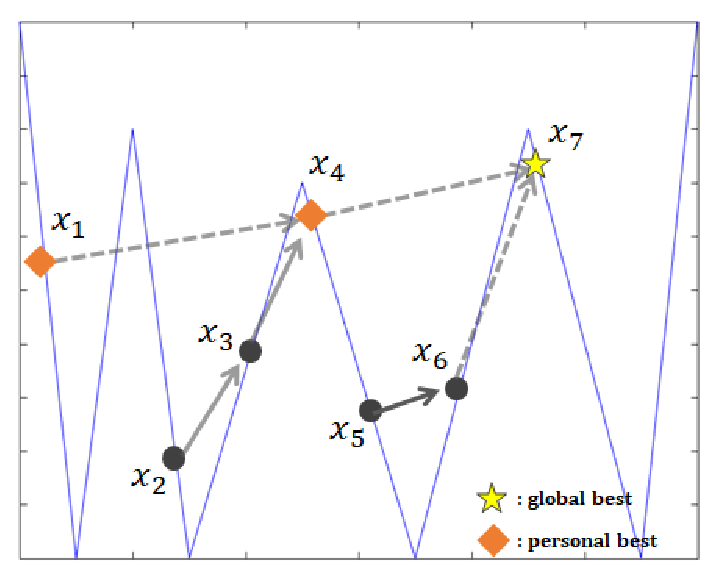
\includegraphics[width=0.8\linewidth]{eps/nbc.eps}
\caption{an example of NBC}
\label{fig:nbc}
\end{figure}

\begin{algorithm}[H]
\caption{Nearest-better clustering (NBC)}
\label{code:nbc}
\begin{algorithmic}[3]
\STATE Calculate all search points mutual distances
\STATE Create an empty graph with num (search points) nodes
\FOR{the search points}
\STATE Find nearest search point that is better, create edge to it
\ENDFOR
\STATE Delete edges of length $> \phi \cdot$ mean(length of all edges)
\STATE Find connected components 
\end{algorithmic}
\end{algorithm}

\subsection{Parameterless-Niching-Assisted NSGAII (PNA-NSGAII)}
\label{ss:PNA-NSGA}
多目的最適化問題によく用いられるNSGA-IIだが,ここでは単目的の最適化問題に対して,どのような問題に対しても適応できるノンパラメトリックなPNA-SNGAII \cite{PNA-NSGA}について説明する.

最適解数に対して同じ個体数を用いることが理想的であるため,ここでは次式で個体数を決定する.
\begin{equation}
T^D=N \Rightarrow T \simeq [e^{\frac{InN}{D}}]
\end{equation}

niching distance $v_d$を次式で求める.
\begin{equation}
v_d=\frac{x_d^{(U)}-x_d^{(L)}}{T} \forall d=\{ 1,2,...,D\}
\end{equation}

\begin{equation}
|(x_1-x_2)_d| \leq \forall d = \{1,2,...,D\}
\end{equation}


% \begin{cases}
$(f_m(x_1) \leq f_m(x_2) \forall_m) \wedge (\exists_n | f_n(x_1) < f_n(x_2)), \ {\rm proximate}(x_1, x_2) = 1   {\rm if }  x_1 \succ x_2 $ \\
$x_1 \ {\rm and} \ x_2 \ {\rm are \ non dominated}  {\rm otherwise}$
% \end{cases}




\newpage
\section{多峰性最適化問題}
\label{sec:MOP}
最適化問題において,実問題の複雑さを多峰性と見立てた評価関数を用いることが一般的である.その代表的な多峰性関数を次節で説明する.


\subsection{最小化問題における評価関数}
\label{ss:MinFunc}
実験で用いられる評価関数の最適解の評価値,最適解数,探索範囲を表\ref{tab:minMOP}に示す.

\begin{description}
\item[$F_1$: Griewank (2D)]\mbox{}\\
Griewank関数 \cite{MOP} の概形を図\ref{fig:minF1}に示し,関数式は次式で表される.
\begin{equation}
\label{eq:minF1}
F_1(x_i)=\sum_{i=1}^D \frac{x_i}{4000}- \prod_{i=1}^D \cos(\frac{x_i}{\sqrt{i}})+1.
\end{equation}
解空間の探索領域は$x_i \in [-10, \ 10]$である$(i=1,2)$.最適解の座標は$x_*=[0, \ 0]$で,その評価値は$F(x_*)=0$である.局所解の座標は$\pm x \approx [6.2800, \ 8.8769], [3.1400, \ 4.4385]$, \\ $[0, \ 8.8769],$  $ [6.2800, \ 0], [9.4200, \ 4.4385]$となる.
\begin{figure}[t]
\centering
\subfigure[Fitness Landscape]{
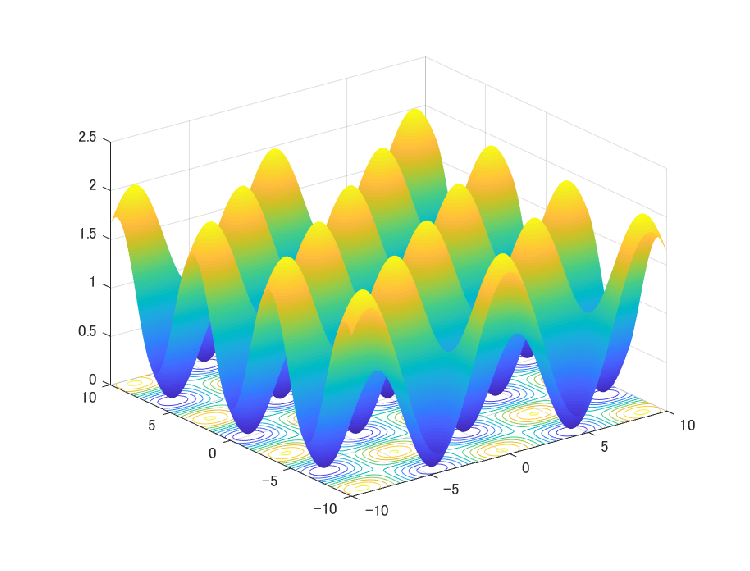
\includegraphics[width=0.8\linewidth]{eps/3d_griewank.eps}
\label{fig:minF1(3d)}}
\subfigure[Contour Plot]{
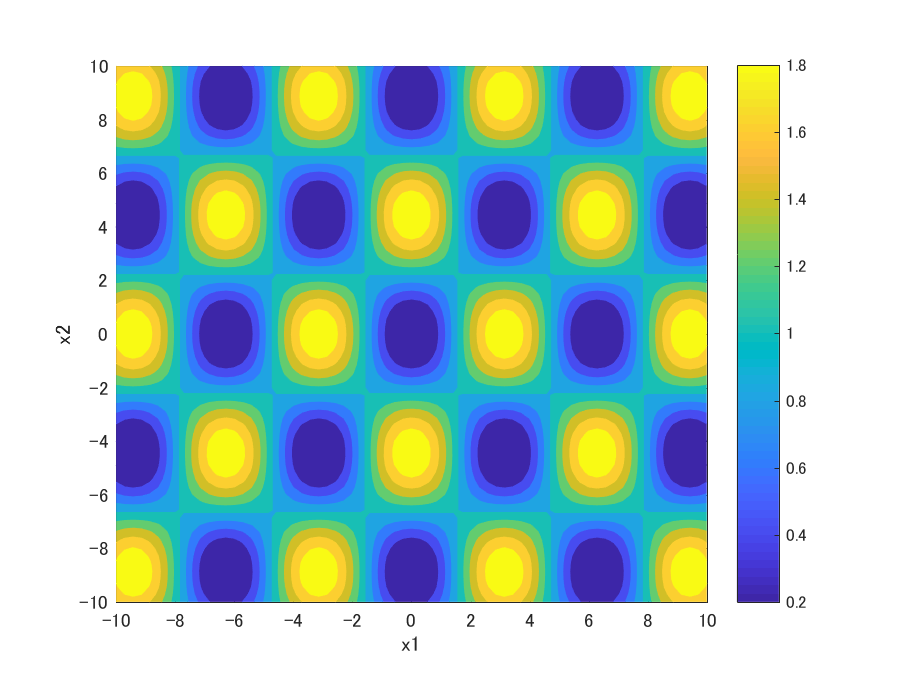
\includegraphics[width=0.8\linewidth]{eps/cont_griewank.eps}
\label{fig:minF1(2d)}}
\caption{Griewank}
\label{fig:minF1}
\end{figure}

\item[$F_2$: Rastrigin (2D)]\mbox{}\\
Rastrigin関数 \cite{MOP} の概形を図\ref{fig:minF2}に示し,関数式は次式で表される.
\begin{equation}
\label{eq:minF2}
F_2(x_i)=10D+\sum_{i=1}^D[x_i^2-10\cos(2\pi x_i)].
\end{equation}
$D$は次元数であり,探索領域は$x_i \in [-5, \ 5]$である.
\begin{figure}[t]
\centering
\subfigure[Fitness Landscape]{
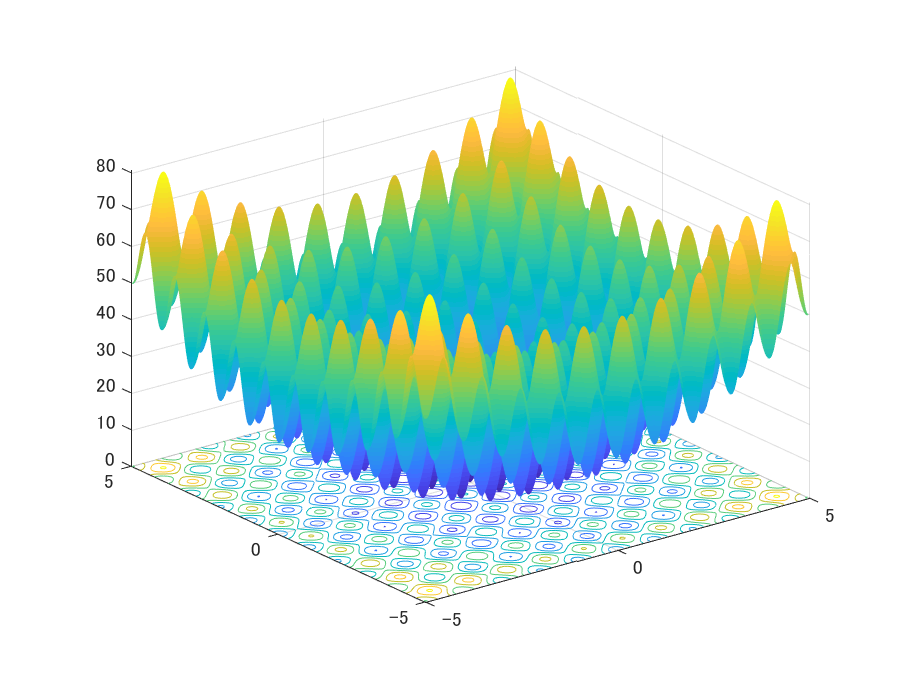
\includegraphics[width=0.8\linewidth]{eps/3d_rastrigin.eps}
\label{fig:minF2(3d)}}
\subfigure[Contour Plot]{
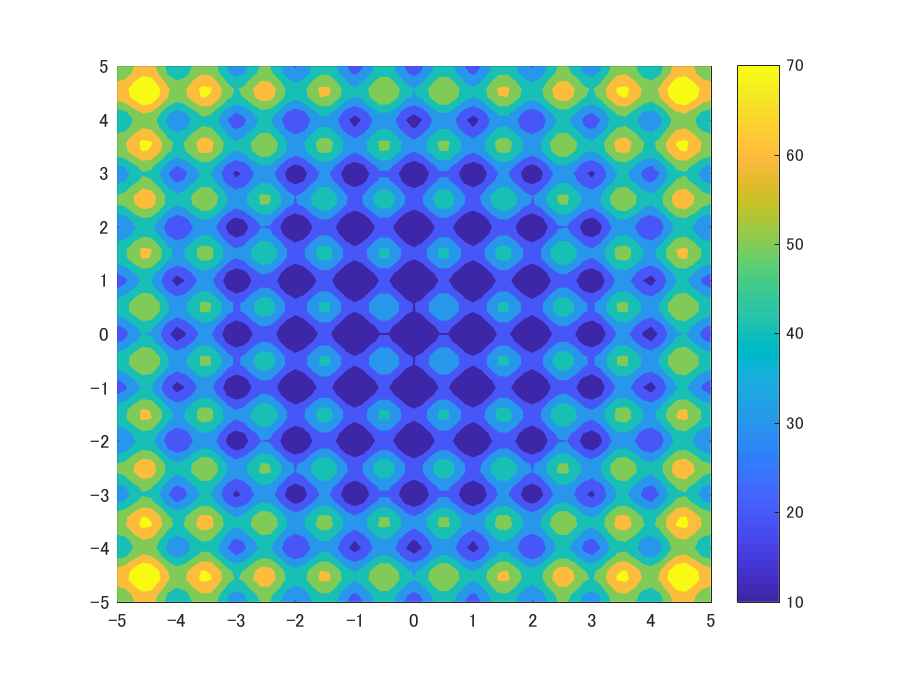
\includegraphics[width=0.8\linewidth]{eps/cont_rastrigin.eps}
\label{fig:minF2(2d)}}
\caption{Rastrigin}
\label{fig:minF2}
\end{figure}

\item[$F_3$: Six-Hump Camel (2D)]\mbox{}\\
最適解と局所解が各2個存在するSix-Hump Camel Function \cite{MOP} は以下の式で表される.
\begin{equation}
\label{eq:minF3}
F_3(x_1,x_2)=(4-2.1x_1^2+ \frac{x_1^4}{3})x_1^2+x_1x_2+(-4+4x_2^2)x_2^2
\end{equation}
この関数における解空間の探索領域は$x_1 \in [-2, \ 2]$, \ $x_2 \in [-1, \ 1]$である.最適解の座標は$x_*=[0.0898, \ -0.7126], [-0.0898, \ 0.7126]$であり,その評価値は$F_3(x_*)=-1.0316$である.また局所解は$\pm x \approx [1.704, \ -0.7965]$に位置する.
\begin{figure}[t]
\centering
\subfigure[Fitness Landscape]{
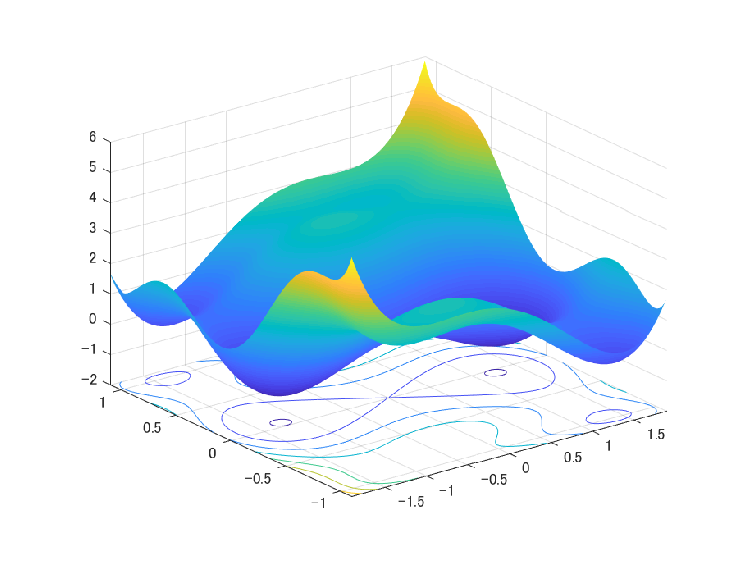
\includegraphics[width=0.8\linewidth]{eps/3d_sixhump_camel.eps}
\label{fig:minF3(3d)}}
\subfigure[Contour Plot]{
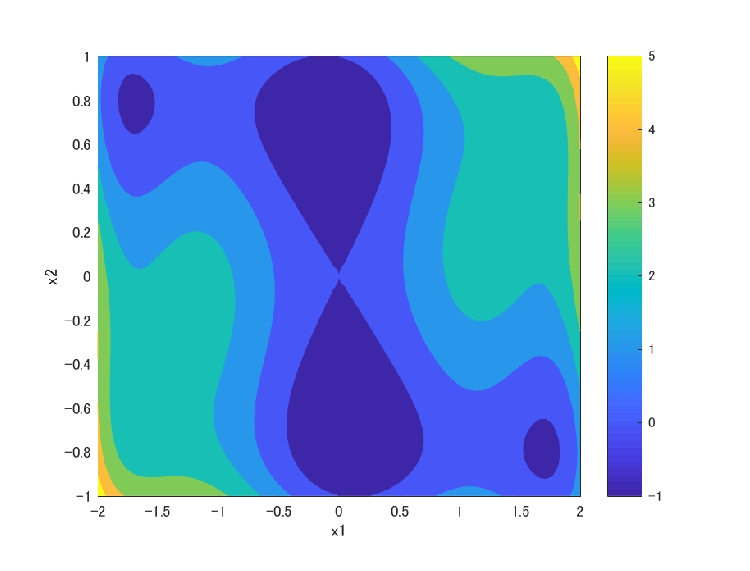
\includegraphics[width=0.8\linewidth]{eps/cont_sixhump_camel.eps}
\label{fig:minF3(2d)}}
\caption{Six-Hump Camel}
\label{fig:minF3}
\end{figure}

\item[$F_4$: Michalewicz (2D)]\mbox{}\\
Michalewicz Function \cite{MOP} の数式を以下に示す.
\begin{equation}
\label{eq:minF4}
F_4(x_i)=- \sum_{i=1}^D \sin(x_i)\sin^{2m}(\frac{ix_i^2}{\pi})
\end{equation}
最適解$x_*=[2.20, \ 1.57]$の評価値$F_3(x_*)=-1.8013$であり,局所解は$x \approx [2.203 \ 2.7115]$である.探索領域は$x_i \in [0, \ 4]$である($i=1,2$).
\begin{figure}[t]
\centering
\subfigure[Fitness Landscape]{
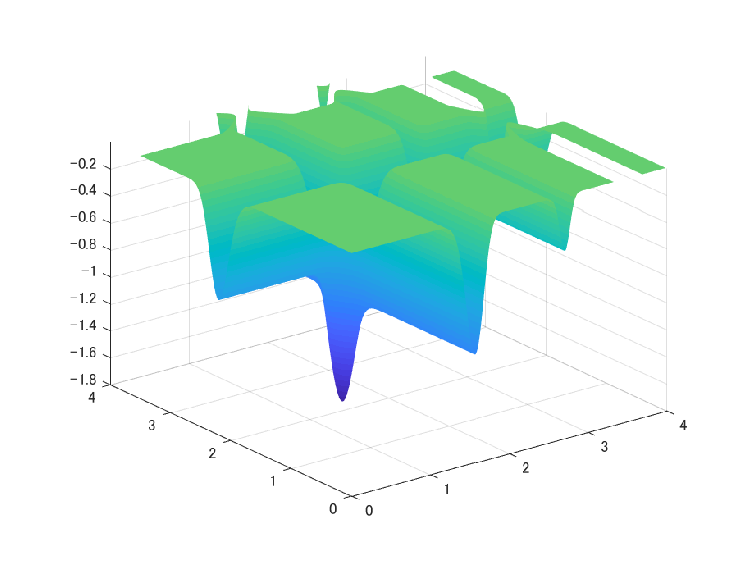
\includegraphics[width=0.8\linewidth]{eps/3d_michalewicz.eps}
\label{fig:minF4(3d)}}
\subfigure[Contour Plot]{
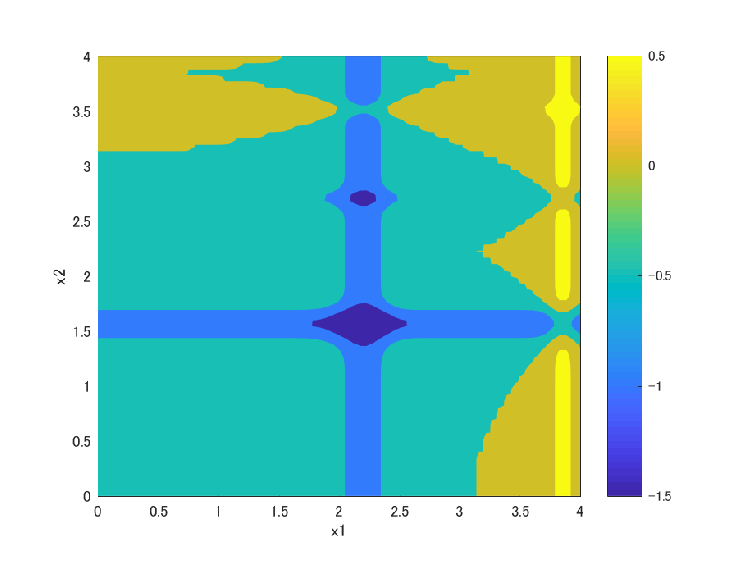
\includegraphics[width=0.8\linewidth]{eps/cont_michalewicz.eps}
\label{fig:minF4(2d)}}
\caption{Michalewicz}
\label{fig:minF4}
\end{figure}

\item[$F_5$: Himmelblau (2D)]\mbox{}\\
Himmelblau Function \cite{himmelblau} の関数式は次の通りとなる.
\begin{equation}
\label{eq:minF5}
F_5(x_1,x_2)=(x_1^2+x_2-11)^2+(x_1+x_2^2-7)^2
\end{equation}
評価関数に局所解は存在せず,最適解のみ4個持つ関数である.最適解の位置は各々$x_*=[3, \ 2]$,$[-2.805118, \ 3.283186]$,$[-3.779310,$  \ $-3.283186],$ $[3.584458, \ -1.848126]$にあり,その評価値は$F_4(x_*)=0$である.探索領域は$x_i \in [-5, \ 5]$となる($i=1,2$).
\begin{figure}[t]
\centering
\subfigure[Fitness Landscape]{
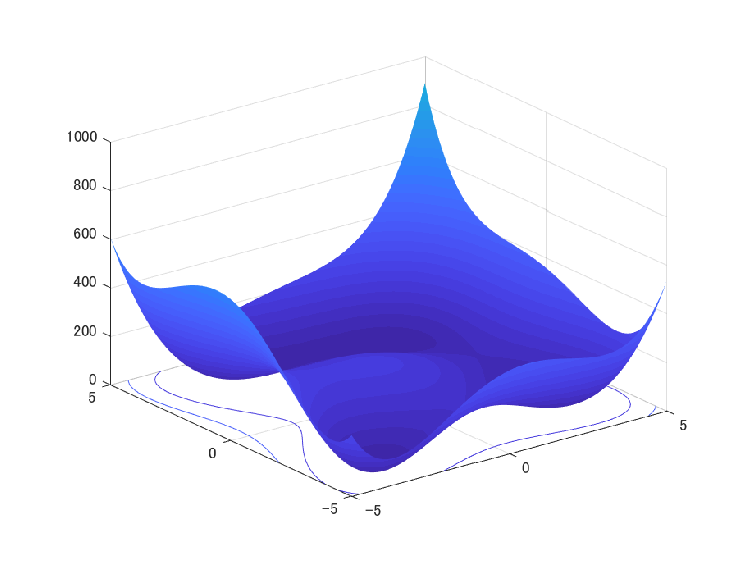
\includegraphics[width=0.8\linewidth]{eps/3d_himmelblau.eps}
\label{fig:minF5(3d)}}
\subfigure[Contour Plot]{
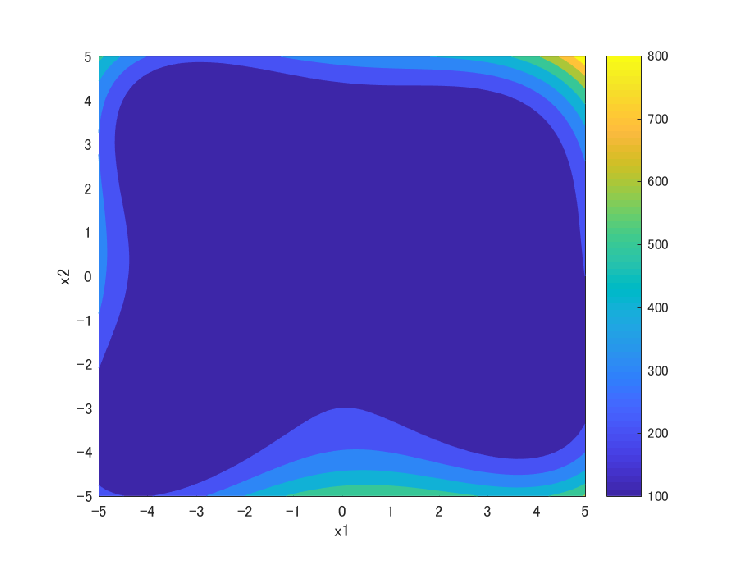
\includegraphics[width=0.8\linewidth]{eps/cont_himmelblau.eps}
\label{fig:minF5(2d)}}
\caption{Himmelblau}
\label{fig:minF5}
\end{figure}

\item[$F_6$: Shubert Function]\mbox{}\\
Shubert関数の概形及び等高線を図\ref{fig:minF6}に示す.
 \begin{equation}
F_6(x_i) = \prod_{i=1}^D \sum_{j=1}^5 j \cos[(j+1)x_i+j], 
\end{equation}
$D$は次元数を表し,最適解の評価値は${F(x_*)=-187.731}$である.この関数では$D \cdot 3^D $個の最適解のみ存在し,2次元では18個の最適解を持つ.探索範囲は$x_i \in [-10, 10]^D$ $(i=1,2,...,D)$である.
\begin{figure}[h]
\centering
\subfigure[Fitness landscape]{
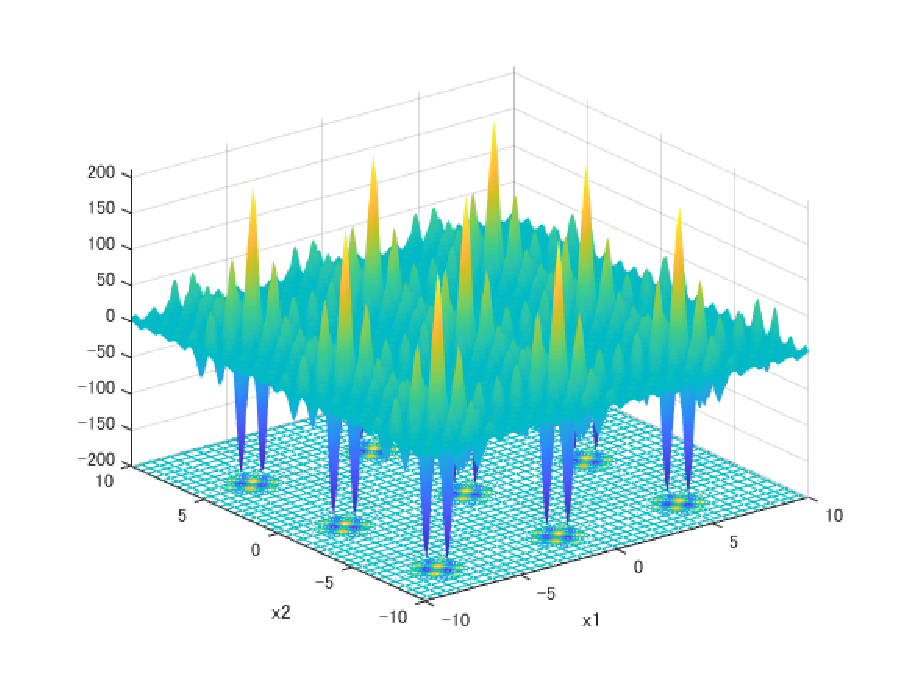
\includegraphics[width=0.8\linewidth]{eps/3d_shubert.eps}
\label{fig:minF6(3d)}}
\subfigure[Contour plot]{
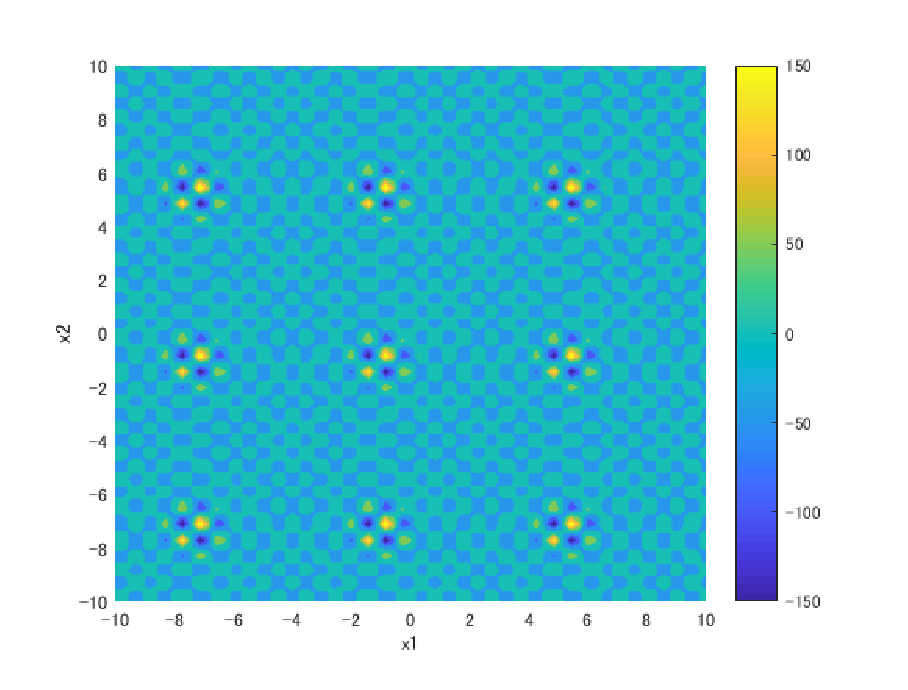
\includegraphics[width=0.8\linewidth]{eps/cont_shubert.eps}
\label{fig:minF6(2d)}}
\caption{$F_6$: Shubert}
\label{fig:minF6}
\end{figure}
\end{description}

\begin{table}[h]
\caption{Benchmark Test Functions}
\begin{center}
\begin{tabular}{c|c|c|c|c|c}
\hline

Function & $F(x*)$ & Num of & Num of & $D$ & Search Range \\
& & goptima & loptima & & \\
\hline
$F_1$ & 0 & 1 & 16 &  2 & $x_i \in [-10,10]$  \\
\hline
$F_2$ & 0 & 1 & 120 & 2 & $x_i \in [-5,5]$  \\
\hline
$F_3$ & -1.0316 & 2 & 2 & 2 & $x_1 \in [-2,2]$  \\
& & & & & $x_2 \in [-1,1]$ \\
\hline
$F_4$ & -1.8013 & 1 & 2 & 2 & $x_i \in [0,4]$  \\
\hline
$F_5$ & 0 & 4 & 0 & 2 & $x_i \in [-5,5]$, \\
\hline
$F_6$ & -187.731 & 18 & many & 2 & $x_i \in [-10,10]$, \\
\hline
\end{tabular}
\label{tab:minMOP}
\end{center}
\end{table}


\FloatBarrier
\subsection{最大化問題における評価関数}
\label{ss:maxFunc}
本実験では,複数最適解を探索する手法の性能を比較するため,CEC ({\it IEEE Congress on Evolutionary Computation}) 2013 Competition on Niching Methods for Multimodal Function Optimization \cite{CEC2013} で扱われたベンチマーク関数を説明する.ベンチマーク関数の最適解の評価値$F(x_*)$と最適解数,探索領域を表\ref{tab:maxMOP}に示す.
\begin{description}
\item[$G_1$: Five-Uneven-Peak Trap (1D)]\mbox{}\\
\begin{equation}
\label{eq:maxF1}
G_1(x)=\begin{cases}
80(2.5-x) & {\rm for} \ 0 \leq x < 2.5, \\
64(x-2.5) & {\rm for} \ 2.5 \leq x < 5.0, \\
64(7.5-x) & {\rm for} \ 5.0 \leq x < 7.5, \\
28(x-7.5) & {\rm for} \ 7.5 \leq x < 12.5, \\
28(17.5-x) & {\rm for} \ 12.5 \leq x < 17.5, \\
32(x-17.5) & {\rm for} \ 17.5 \leq x < 22.5, \\
32(27.5-x) & {\rm for} \ 22.5 \leq x < 27.5, \\
80(x-27.5) & {\rm for} \ 27.5 \leq x < 30.
\end{cases}
\end{equation}
\begin{figure}[h]
\centering
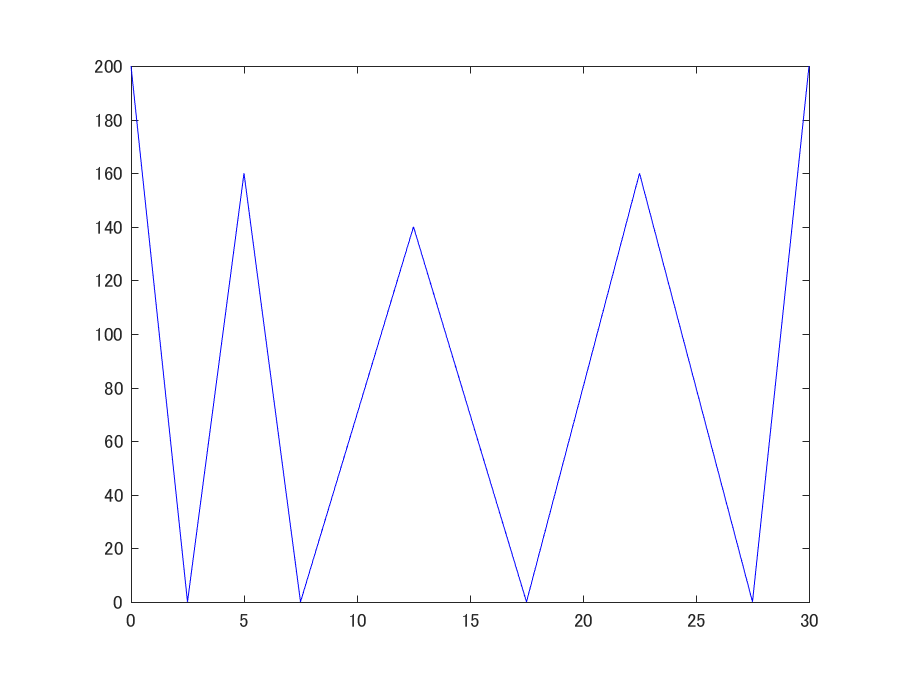
\includegraphics[width=0.8\linewidth]{eps/F1.eps}
\caption{Five-Uneven-Peak Trap}
\label{fig:maxF1}
\end{figure}

\item[$G_2$: Equal Maxima (1D)]\mbox{}\\
\begin{equation}
\label{eq:maxF2}
G_2(x)=\sin^6{(5\pi x)}.
\end{equation}
\begin{figure}[h]
\centering
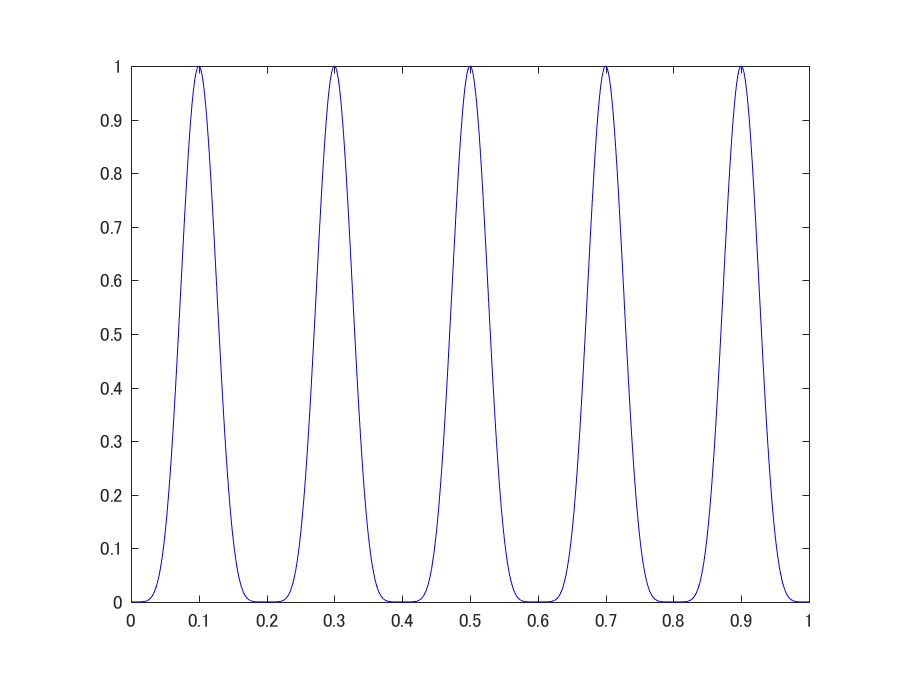
\includegraphics[width=0.8\linewidth]{eps/F2.eps}
\caption{Equal Maxima}
\label{fig:maxF2}
\end{figure}

\item[$G_3$: Uneven Decreasing Maxima (1D)]\mbox{}\\
\begin{equation}
\label{eq:maxF3}
G_3(x)=exp(-2log(2)(\frac{x-0.08}{0.854})^2)\sin^6{(5\pi(x^{\frac{3}{4}}-0.05))}.
\end{equation}
\begin{figure}[h]
\centering
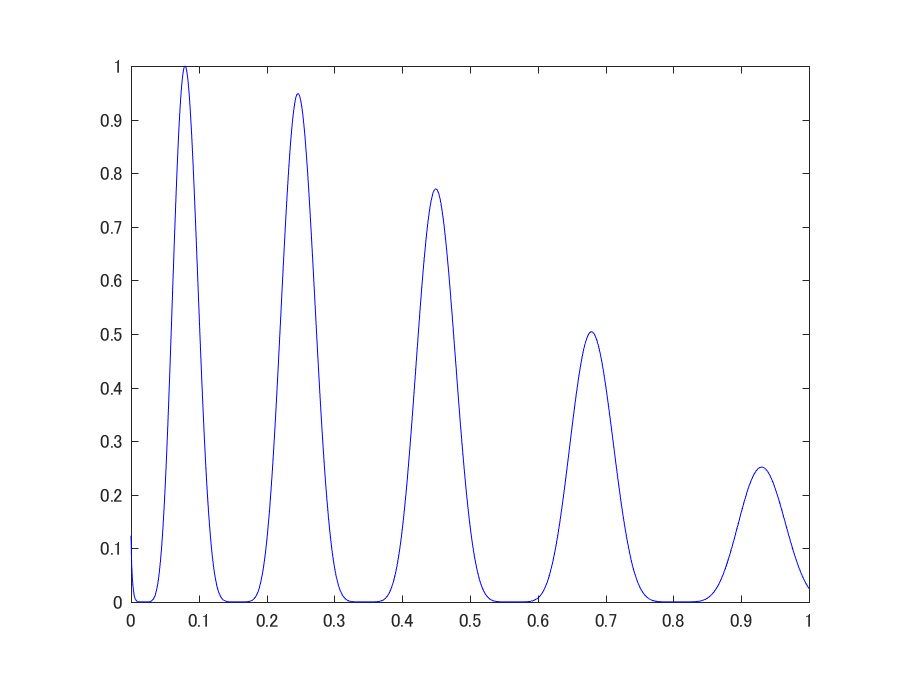
\includegraphics[width=0.8\linewidth]{eps/F3.eps}
\caption{Uneven Decreasing Maxima}
\label{fig:maxF3}
\end{figure}

\item[$G_4$: Himmelblau (2D)]\mbox{}\\
\begin{equation}
\label{eq:maxF4}
G_4(x,y) = 200 - (x^2+y-11)^2 - (x+y^2-7)^2.
\end{equation}
\begin{figure}[h]
\centering
\includegraphics[width=0.8\linewidth]{eps/F4.eps}
\caption{2D Himmelblau}
\label{fig:maxF4}
\end{figure}

\item[$G_5$: Six-Hump Camel Back (2D)]\mbox{}\\
\begin{equation}
\label{eq:maxF5}
G_5(x,y)=-4[(4-2.1x^2+\frac{x^4}{3})x^2+xy+(4y^2-4)y^2].
\end{equation}
\begin{figure}[h]
\centering
\includegraphics[width=0.8\linewidth]{eps/F5.eps}
\caption{2D Six-Hump Camel Back}
\label{fig:maxF5}
\end{figure}

\item[$G_6$: Shubert (2D)]\mbox{}\\
\begin{equation}
\label{eq:maxF6}
G_6(x)=-\prod_{i=1}^D \sum_{j=1}^5 j\cos[(j+1)x_i+j].
\end{equation}
\begin{figure}[h]
\centering
\includegraphics[width=0.8\linewidth]{eps/F6.eps}
\caption{2D Shubert}
\label{fig:maxF6}
\end{figure}

\end{description}

\begin{table}[h]
\caption{Benchmark Test Functions}
\begin{center}
\begin{tabular}{c|c|c|c|c|c}
\hline

Function & $G(x_*)$ & Num of & $\rho$ & $D$ & Search Range \\
& & goptima & & & \\
\hline
$G_1$ & 200.0 & 2 & 0.01 & 1 & $x \in [0,30]$  \\
\hline
$G_2$ & 1.0 & 5 & 0.01 & 1 & $x \in [0,1]$  \\
\hline
$G_3$ & 1.0 & 1 & 0.01 & 1 & $x \in [0,1]$  \\
\hline
$G_4$ & 200.0 & 4 & 0.01 & 2 & $x,y \in [-6,6]$  \\
\hline
$G_5$ & 1.03163 & 2 & 0.5 & 2 & $x \in [-1.9,1.9]$, \\
& & & & & $y \in [-1.1,1.1]$ \\
\hline
$G_6$ & 186.731 & 18 & 0.5 & 2 & $x_i \in [-10,10]$  \\
\hline
% \multicolumn{4}{l}{$^{\mathrm{a}}$Sample of a Table footnote.}
\end{tabular}
\label{tab:maxMOP}
\end{center}
\end{table}

% \subsection{月面着陸地点選定問題}
% \label{ss:LSM}
% 実問題の一例として,進化計算シンポジウムコンペティション2018で取り上げられた月着陸における最適着陸地点選定問題 \cite{ECCompetition} が挙げられる.

\clearpage
\newpage
\section{Novelty Search-based Bat Algorithm (NSBA)}
\label{sec:NSBA}
本章では多峰性最適化に対し,大域探索と局所探索を自動で切り替えることに優れたBat Algorithm (BA) と,未探索領域に解を生成するNovelty Searchを組み合わせたNSBA \cite{NSBA} を説明する.
% この章では\proposed で用いるDCAの基礎となるニューラルネットワーク及びディープラーニングを扱う.
% はじめに階層型ニューラルネットワークとその学習方法を\ref{ss:NN}{}節で説明し, その学習方法を\ref{ss:bpg}節で説明する.
% 次にニューラルネットワークを利用した機構である自己符号化器(オートエンコーダー)\cite{AE}を\ref{ss:AE}節で説明し, 最後に深いニューラルネットワークの学習である深層学習を\ref{ss:DL}節で説明する.

\subsection{Novelty Search}
\label{ss:NS}
Novelty Search \cite{NS} は未探索領域に新たに解を生成することを目的とした手法である.個体間距離の算出式は次式で表される.
\begin{equation}
\label{eq:ns}
\rho(x)=\frac{1}{k}\sum_{i=1}^k dist(x,\mu_i)
\end{equation}
この時,$\rho(x)$は個体$x$における密度を表しており,$kは$個体$x$の近傍数,$dist$は個体$x$と$\mu_i$の距離を表す.図\ref{fig:ns}は近傍数が3の時の解の生成を表す.
\begin{figure}[h]
  \centering
  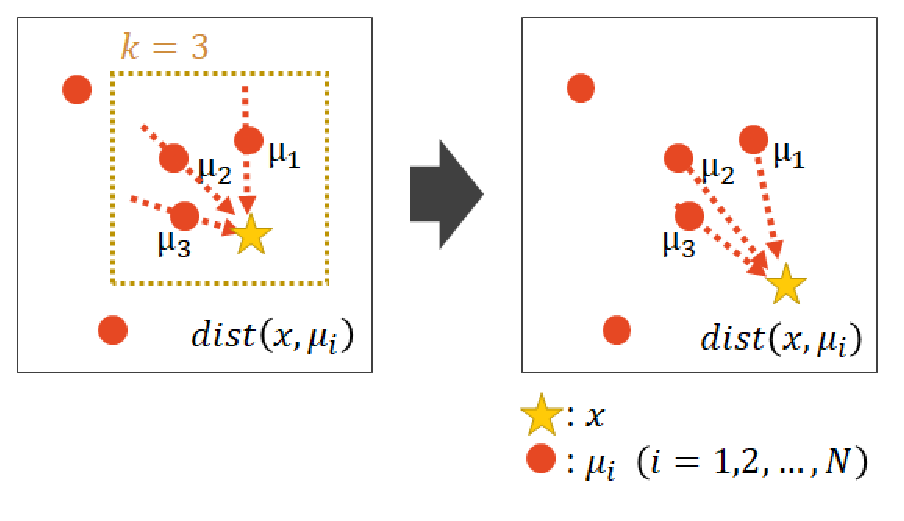
\includegraphics[width=0.8\linewidth]{eps/IES2018/ns.eps}
  \caption{解候補の生成}
  \label{fig:ns}
\end{figure}

\subsection{メカニズム}
\label{ss:NSBA-abst}
NSBAはBAにNovelty Searchを組み込んだ複数解探索手法であり,BAからの変更点を図\ref{fig:nsba_table}に表す.(\ref{eq:ns})式を以下のベクトル式に変更することで,密集している個体が疎な方向へ新たに解候補を生成する.

\begin{figure}
  \centering
  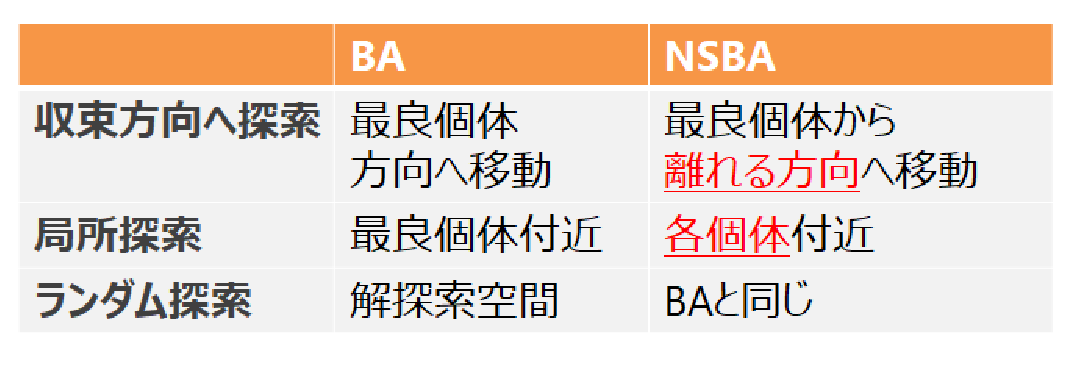
\includegraphics[width=0.7\linewidth]{eps/nsba_table.eps}
  \caption{BAからの変更点}
  \label{fig:nsba_table}
\end{figure}
\begin{equation}
\mbox{\boldmath $d_i^{t}$} = \frac {1}{N} \sum _{j=1}^N \frac {(\mbox{\boldmath $x_{pbest}$}-\mbox{\boldmath $x_j^{t}$})}{|\mbox{\boldmath $x_{pbest}$}-\mbox{\boldmath $x_j^{t}$}|^2}
\label{eq:nd*}
\end{equation}
\begin{equation}
\mbox{\boldmath $v_i^{t+1}$}=\mbox{\boldmath $v_i^{t}$}+\mbox{\boldmath $d_i^{t}$}*f_i
\label{eq:nsvi}
\end{equation}
この時,$x_{pbest}$は$i$番目の最良個体を表し,このベクトル式から速度$v_i$を更新する.

局所探索では,最良個体$x_{pbest}$付近に新たに解候補を次式で生成される.
\begin{equation}
\mbox{\boldmath $x_{loc}$}=\mbox{\boldmath $x_{pbest}$} + \epsilon A^t,
\label{eq:ns_xloc}
\end{equation}
$\epsilon$は$[-1, \ 1]$区間におけるD次元の一様乱数を表す.
ランダム探索では,探索空間内に新たに解候補を生成する.
\begin{equation}
\mbox{\boldmath $x_{rnd}$} = x_{lb} + (x_{ub} - x_{lb})* rand(1, \ D)
\label{eq:ns_rnd}
\end{equation}

\subsection{アルゴリズム}
\label{ss:NSBA-algorithm}
アルゴリズムの疑似コードを以下のAlgorithm \ref{code:nsba}に記す.

\begin{itemize}
\item {\bf STEP1: 個体の初期化}\\
探索空間内にランダムに個体$x_i (i=1,2,...,N)$を生成し,周波数$f_i$,ラウドネス$A_i^0$,パルスレート$r_i^0$を決定する(1-3行目).
\item {\bf STEP2: 速度の更新と解候補の生成}\\
速度$v_i$により新しく解候補を生成する(6行目).
\item {\bf STEP3: 局所探索}\\
最良解$x_{pbest}$近辺に新しく解候補$x_{loc}$を生成する(8行目).
\item {\bf STEP4: ランダム探索}\\
探索空間内にランダムで解候補$x_{rnd}$を生成する(10行目).
\item {\bf STEP5: 評価と更新}\\
${\rm rand} < A_i$を満たす,かつ3つの解候補が$t$時点での最良解$x_{pbest}$よりも評価値が高ければ解を更新する(11-14行目).
\item {\bf STEP6: STEP2へ戻る}\\
終了条件を満たすまでSTEP2へ戻る.
\end{itemize}

\begin{algorithm}[H]
\caption{Novelty Search-based Bat Algorithm}
\label{code:nsba}
\begin{algorithmic}[6]
\REQUIRE Objective\ Function\ $F(x)$
\STATE Initialize Population $x_i(i=1,2,..., N)$ and $v_i$\\
\STATE Define frequency $f_i$ at location $x_i$ [Eq.(\ref{eq:freq})]
\STATE Initialize pulse rates $r_i$, and loudness $A_i$
\WHILE{($t <$ Max number of iterations)}
\FOR{i=1 to N}
\STATE Generate a new solution $x_i$ and update velocity $v_i$  [Eqs.(\ref{eq:ba-xi})(\ref{eq:nd*})(\ref{eq:nsvi})] 
\IF{($rand>r_i$)}
\STATE Generate a new solution ${x_{loc}}$ around the solution $x_{i}$ [Eq.(\ref{eq:ns_xloc})] 
\ENDIF
\STATE Generate a new solution $x_{rnd}$ randomly (or without ${x_{rnd}}$) [Eq. (\ref{eq:ns_rnd})]
\IF{($rand<A_i \ \& \min (F(x_i), F(x_{new}), F(x_{rnd}))<F(x_{i*})$)}
\STATE Accept the new solution, and update pulse rate $r_i$ \\ \& loudness $A_i$ [Eqs. (\ref{eq:loud})(\ref{eq:pulse})] 
\ENDIF
\ENDFOR
\STATE Evaluate the all bats and select a best solution $x_{i*}$ in the current solutions
\ENDWHILE
\end{algorithmic}
\end{algorithm}

\subsection{実験}
\label{ss:NSBA-exp}
本実験では従来のBAとNSBAの性能を比較するため,代表的な以下の多峰性関数を用いる.

\subsubsection{評価関数}
\label{sss:NSBA-func}
本実験では\ref{ss:MinFunc}節で説明した$F_1$関数(Griewank)と$F_2$関数(Rastrigin)を用いる.


\FloatBarrier

\subsubsection{評価基準}
\label{sss:NSBA-eval}
本実験ではPeak Ratio (PR) \cite{CDE} を採用し,最適解及び局所解の発見率を次式で求める.
\begin{equation}
\label{eq:PR}
PR=\frac{\sum_{run=1}^{MR}FPs}{TP*MR}
\end{equation}
ここで,$TP$は評価関数の全最適解と局所解数(Total Peak)を表し,$MR$は実験回数(Max Run)を表す.$FPs$は発見した解の数(Found Peaks)を表す.解発見の定義はピークとその最近傍個体とのユークリッド距離が0.1未満であった時,その解を発見したとする.

\subsubsection{実験設定}
\label{sss:nsba-setup}
本実験では,$F_1$関数では個体数$N=50,100$,$F_2$関数では$N=100,150$とした.2つの関数において,$f_{max}=1, f_{min}=0$, ラウドネス$A^0=1$, パルスレート$r^0 \in rand[0,1]$とし,$\alpha = \gamma = 0.9$と設定した.世代数は10000,実験回数を30回とした.

\subsubsection{実験結果}
\label{sss:nsba-results}
\begin{itemize}
\item {\bf PRと発見した解数} \\
表\ref{tab:nsba}はBAとNSBAにおける,発見した解の数(FPs)とその発見率(PR)の30試行回数による平均値と標準偏差を示す.表\ref{tab:nsba}より2つの関数に対し,NSBAはBAよりもFPs及びPR値が高いことから探索性能が良好である.図\ref{fig:nsba-results_ba}, \ref{fig:nsba-results_nsba}は最終世代における解の分布を表し,白い丸が解の位置である.図よりBAは一つの最適解に収束する傾向にあるが,一方でNSBAは最適解とその周辺にある複数の局所解に留まっていることが分かった.
\item {\bf 収束速度} \\
図\ref{fig:nsba-all_iter}はNSBAとBAの世代数によるPR値の推移を表しており,縦軸はPR値,横軸は世代数を示す.黒い実線はBA,黒い点線はNSBAの推移を示している.図\ref{fig:nsba-f1_n50}から\ref{fig:nsba-f2_n150}でBAは最終世代において,PR値が0\%付近で収束しているのに対し,NSBAは$F_1$関数では70\%までPR値が上昇し,1000世代以降は徐々に低下する傾向にある.$F_2$関数ではNSBAのPR値が20\%から10\%まで減少し,3000世代以降は停滞する傾向が見られた.
\end{itemize}  

\begin{table}[h]
\caption{Found Peaks and Peak Ratio of BA and NSBA}
\begin{center}
\begin{tabular}{c|c|c|c|c|c|c}
\hline
\multicolumn{1}{c|}{} & \multicolumn{3}{c|}{BA} & \multicolumn{3}{c}{NSBA}  \\
\hline
Function & Mean & SD & PR & Mean & SD & PR \\
\hline
$F_1 \ (N=50)$ & 1.0 & 0 & 5.89 \% & 6.8 & 0.7024 & 40.0 \% \\
\hline
$F_1 \ (N=100)$ & 1.0 & 0 & 5.89 \% & 7.267 & 0.5735 & 42.75 \% \\
\hline
$F_2 \ (N=100)$ & 1.0 & 0 & 0.87 \% & 7.9333 & 0.8929 & 6.56 \% \\
\hline
$F_2 \ (N=150)$ & 1.0 & 0 & 0.87 \% & 8.0667 & 0.7717 & 6.67 \% \\
\hline
\end{tabular}
\label{tab:nsba}
\end{center}
\end{table}

\begin{figure}[t]
\centering
\subfigure[$F_1 :(N=50)$]{
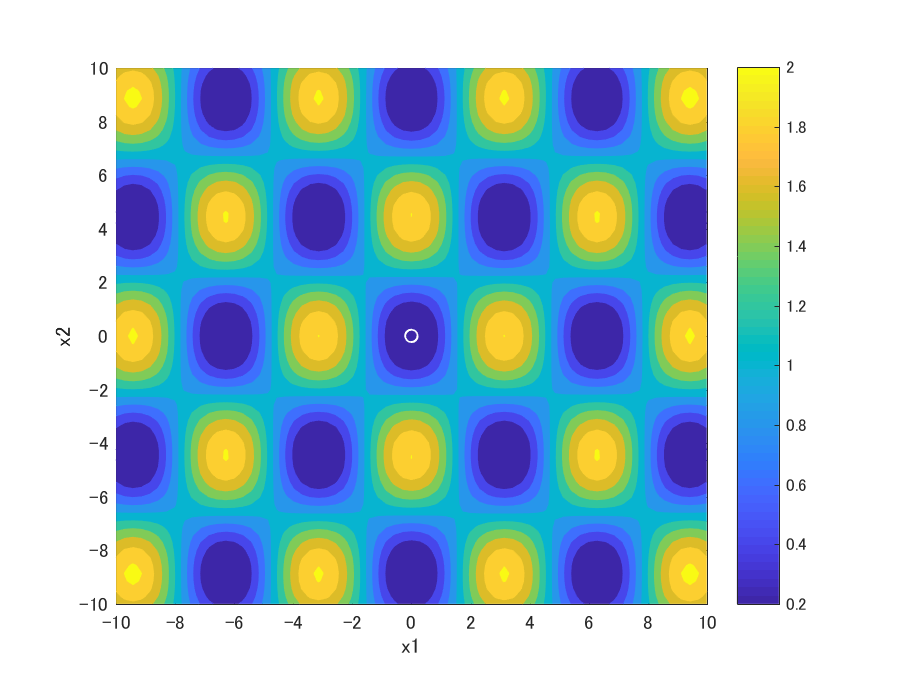
\includegraphics[width=0.8\linewidth]{eps/IES2018/f1_ba50.eps}
\label{fig:nsba-f1_ba50}}
\subfigure[$F_1 :(N=100)$]{
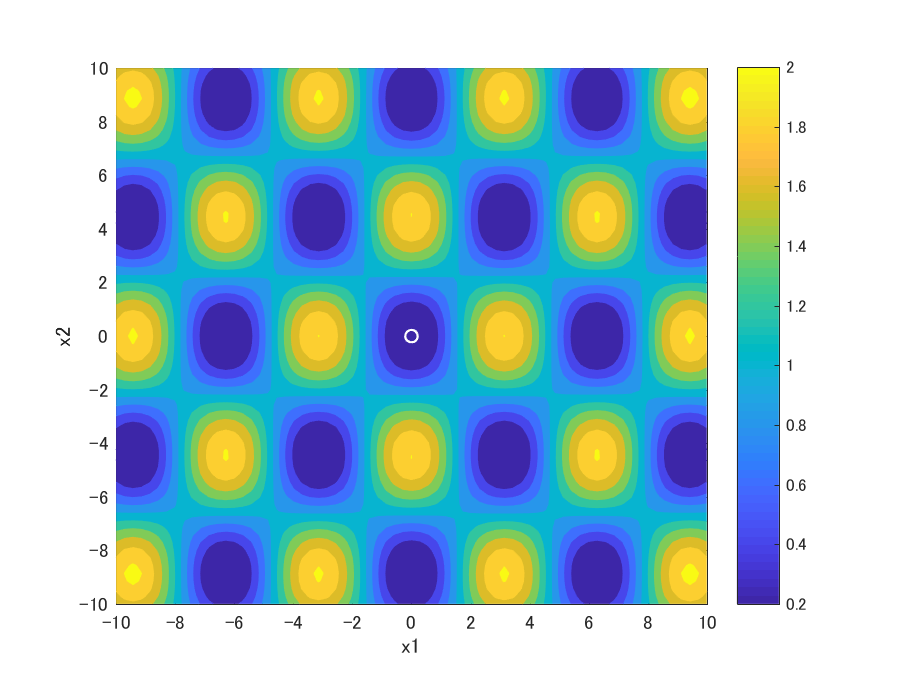
\includegraphics[width=0.8\linewidth]{eps/IES2018/f1_ba100.eps}
\label{fig:nsba-f1_ba100}}
\end{figure}

\begin{figure}[t]
\centering
\subfigure[$F_2 :(N=100)$]{
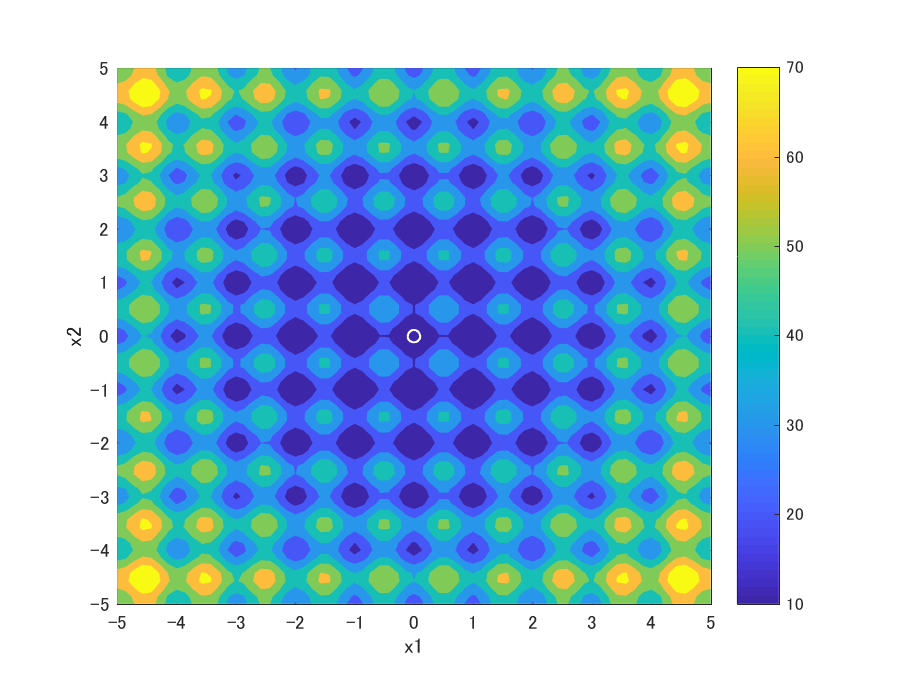
\includegraphics[width=0.8\linewidth]{eps/IES2018/f2_ba100.eps}
\label{fig:nsba-f2_ba100}}
\subfigure[$F_2 :(N=150)$]{
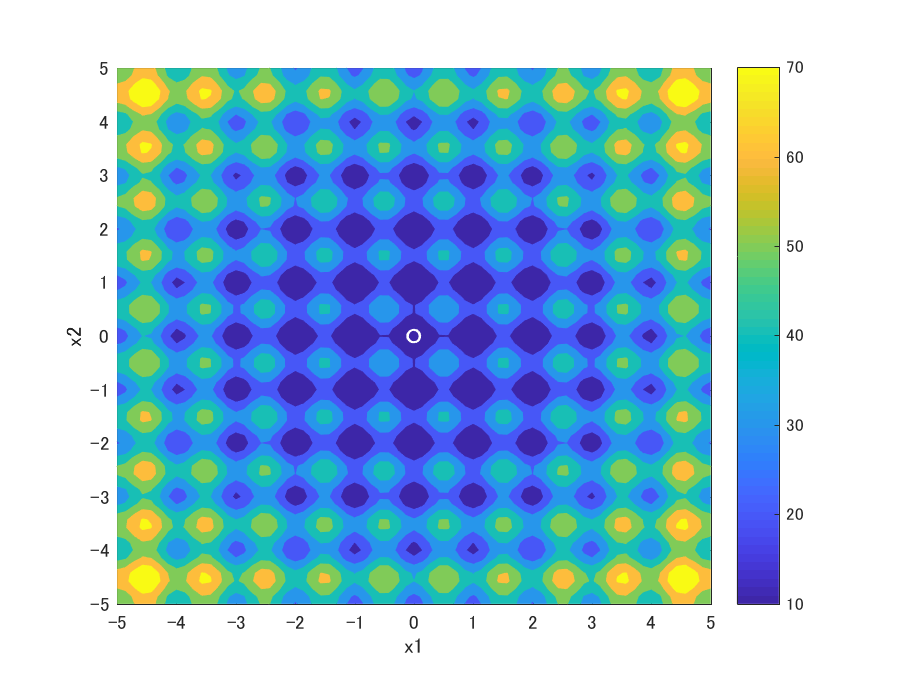
\includegraphics[width=0.8\linewidth]{eps/IES2018/f2_ba150.eps}
\label{fig:nsba-f2_ba150}}
\caption{BA}
\label{fig:nsba-results_ba}
\end{figure}

\begin{figure}[t]
\centering
\subfigure[$F_1 :(N=50)$]{
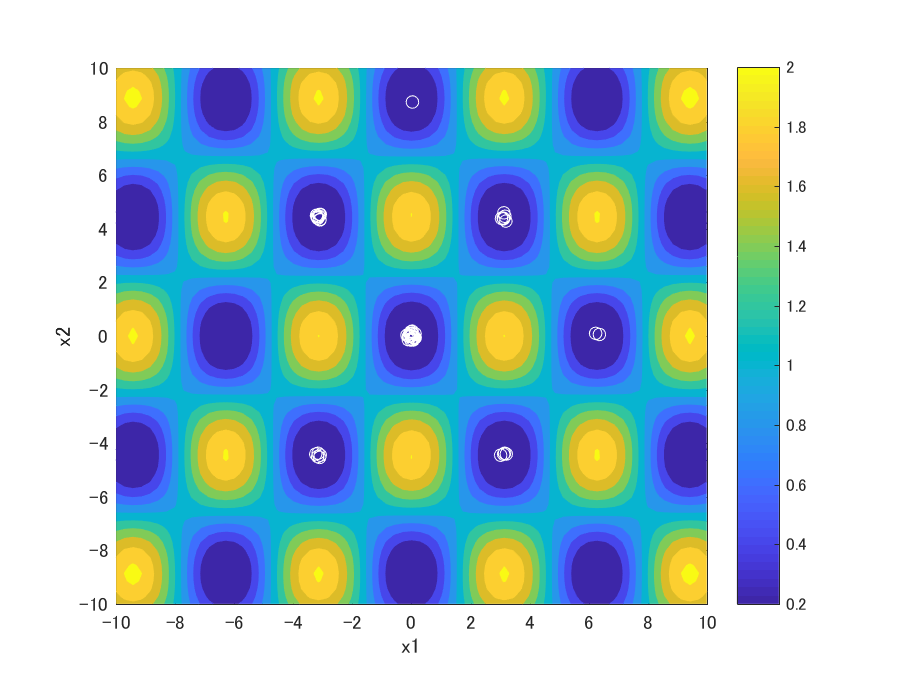
\includegraphics[width=0.8\linewidth]{eps/IES2018/f1_nsba50.eps}
\label{fig:nsba-f1_nsba50}}
\subfigure[$F_1 :(N=100)$]{
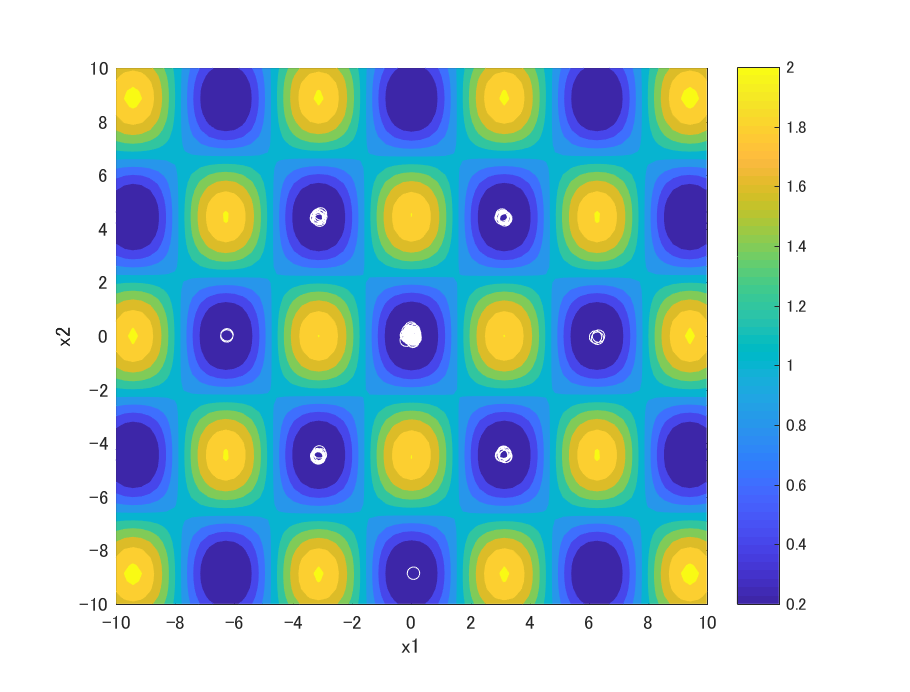
\includegraphics[width=0.8\linewidth]{eps/IES2018/f1_nsba100.eps}
\label{fig:nsba-f1_nsba100}}
\end{figure}

\begin{figure}[t]
\centering
\subfigure[$F_2 :(N=100)$]{
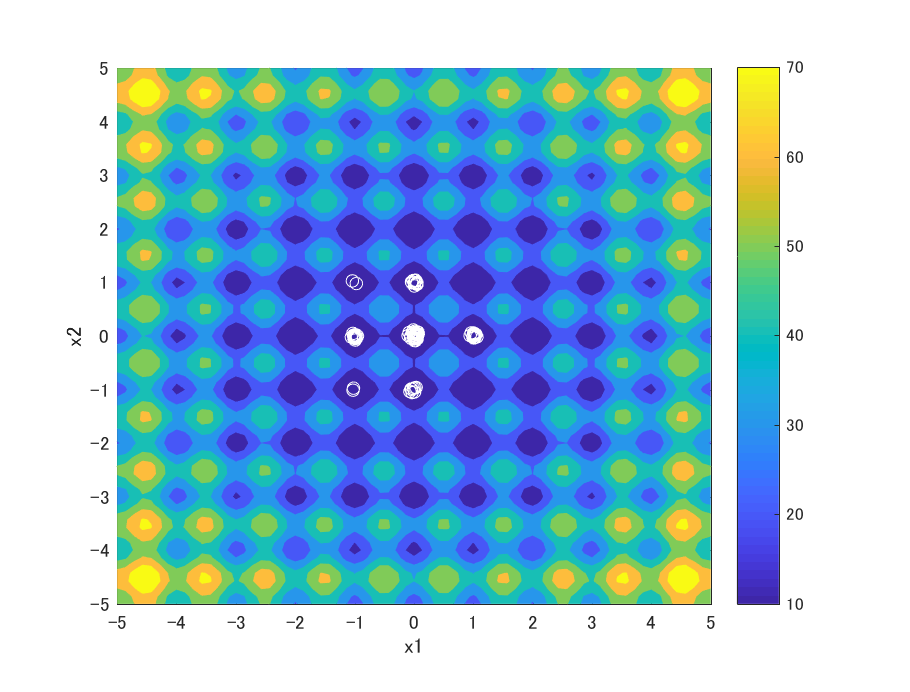
\includegraphics[width=0.8\linewidth]{eps/IES2018/f2_nsba100.eps}
\label{fig:nsba-f2_nsba100}}
\subfigure[$F_2 :(N=150)$]{
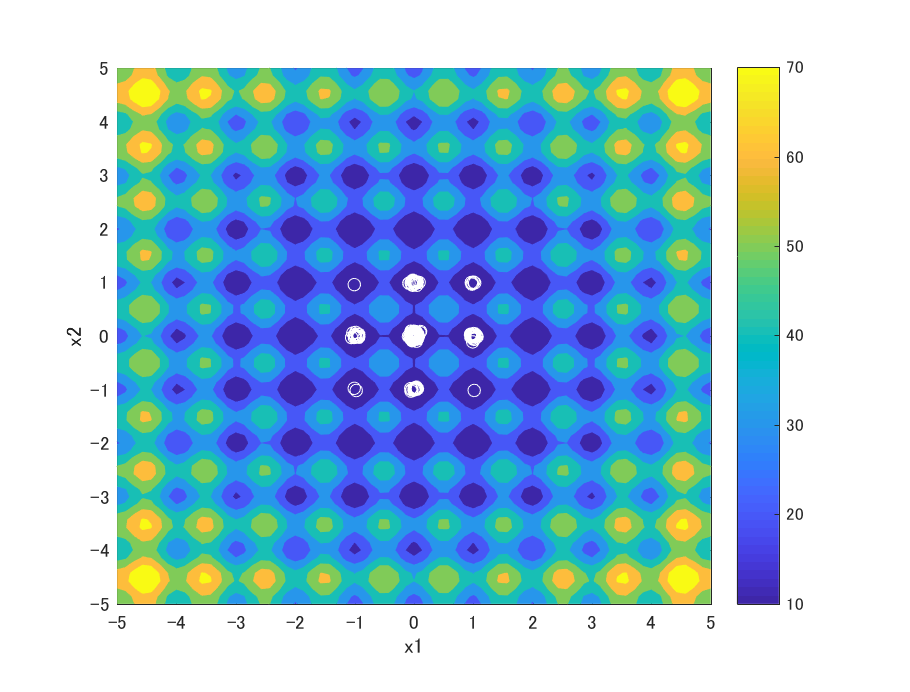
\includegraphics[width=0.8\linewidth]{eps/IES2018/f2_nsba150.eps}
\label{fig:nsba-f2_nsba150}}
\caption{NSBA}
\label{fig:nsba-results_nsba}
\end{figure}

\subsection{考察}
\label{ss:nsba-disc}

\subsubsection{個体数による影響}
個体数の変化による影響があるか調査するため,BAとNSBAにて個体数を変えて実験を行った.表\ref{tab:nsba}より,BAのPR値は$F_1$, $F_2$関数のいずれにおいても個体数による変化がなかった.一方,NSBAは個体数が増加すると2つの関数においてPR値が増加した.NSBAは$F_1$関数において,40\%から42.75\%と探索率が上昇し,$F_2$関数においても6.56\%から6.67\%と僅かに上昇した.このことから個体数を増やすことで探索性能が向上したと考えられる.また,図\ref{fig:nsba-all_iter}からも個体数の増加により,世代数が増す中でPR値を維持していることが分かる.$F_1$関数でNSBA($N=50$)のPR値は70\%から30\%へと低下しているが,NSBA($N=100$)では6000世代付近から50\%を維持していることが分かる.

\begin{figure}[t]
\centering
\subfigure[$F_1 :(N=50)$]{
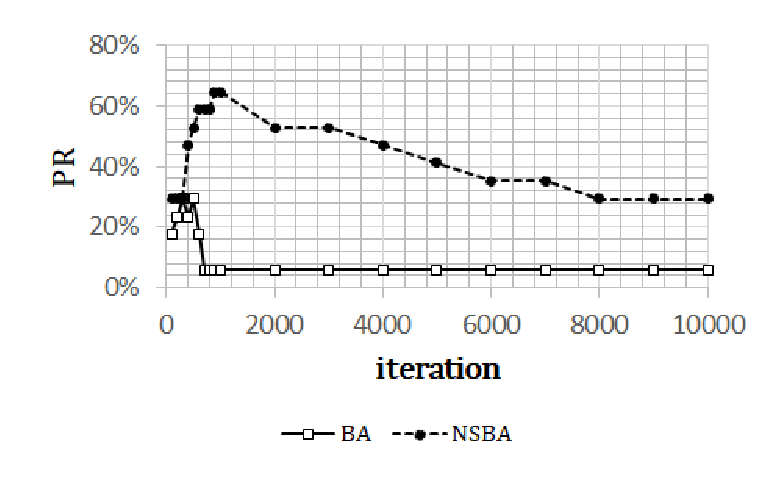
\includegraphics[width=0.8\linewidth]{eps/IES2018/f1_n50.eps}
\label{fig:nsba-f1_n50}}
\subfigure[$F_1 :(N=100)$]{
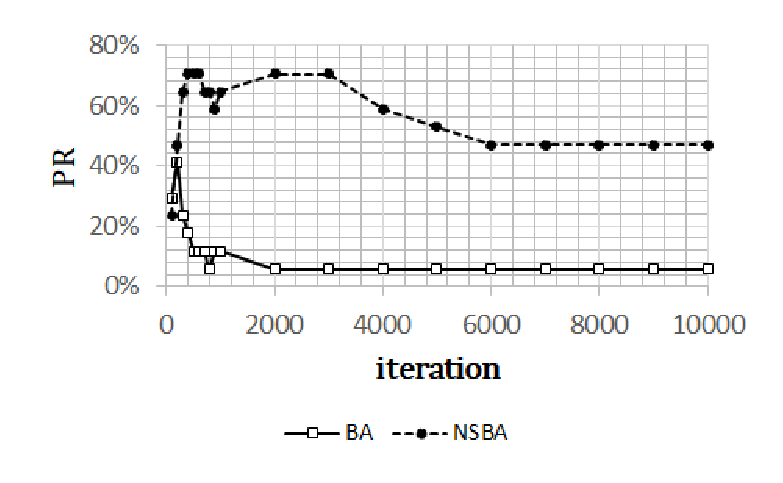
\includegraphics[width=0.8\linewidth]{eps/IES2018/f1_n100.eps}
\label{fig:nsba-f1_n100}}
\end{figure}

\begin{figure}[t]
\centering
\subfigure[$F_2 :(N=100)$]{
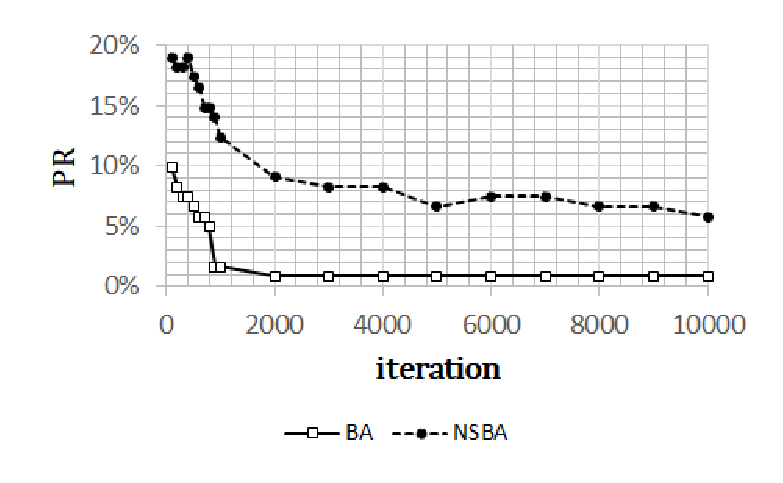
\includegraphics[width=0.8\linewidth]{eps/IES2018/f2_n100.eps}
\label{fig:nsba-f2_n100}}
\subfigure[$F_2 :(N=150)$]{
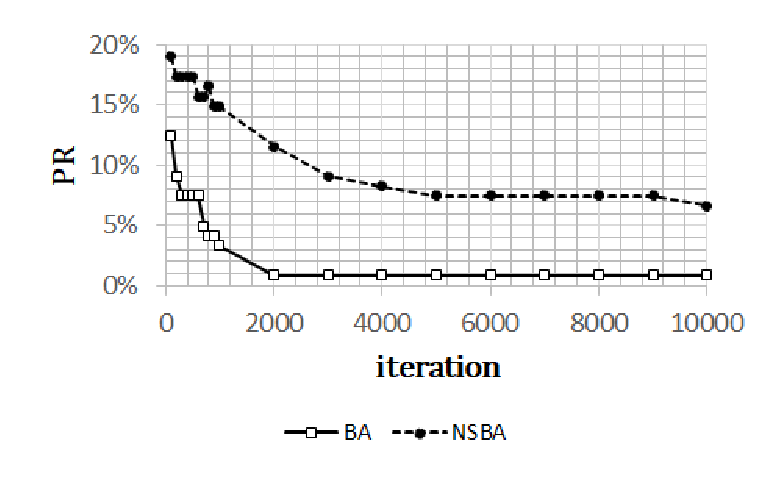
\includegraphics[width=0.8\linewidth]{eps/IES2018/f2_n150.eps}
\label{fig:nsba-f2_n150}}
\caption{Convergence Speed of Peak Ratio implemented by BA and NSBA}
\label{fig:nsba-all_iter}
\end{figure}

\subsubsection{解の分布}
図\ref{fig:nsba-all_iter}よりPR値を維持できない原因を分析するため,ここではPR値が最も高かった1000世代目の解分布に着目し,その時の分布図を図\ref{fig:nsba-results_nsba_1000}に示す.この図から$F_1$関数において,NSBAは1000世代目ではほぼ全ての最適解及び局所解を探索することができているが,図\ref{fig:nsba-all_iter}から1000世代以降にPR値が低下している.これはNSBAの収束性能が強いために,一度発見した解よりも評価値の高い解を見つけた場合に移動してしまうことが原因であると考えられる.$F_2$関数においても同じような傾向が見られたが,$F_1$関数よりも多くの局所解が存在することから探索が困難となり,PR値は探索開始時から最終世代まで,20\%から10\%へと低いPR値であった.

\begin{figure}[t]
\centering
\subfigure[$F_1 :(N=50)$]{
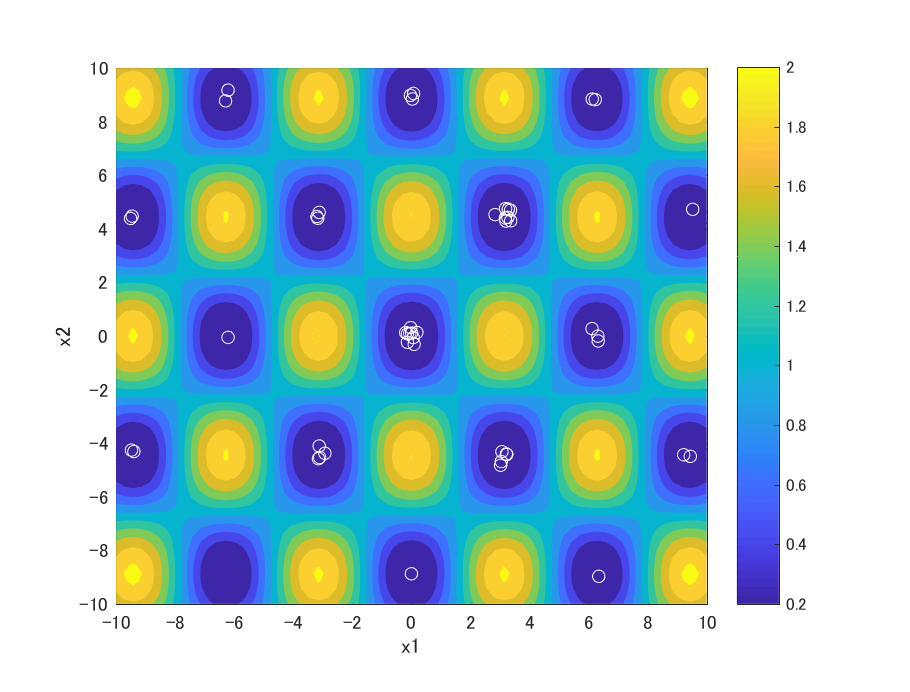
\includegraphics[width=0.8\linewidth]{eps/IES2018/f1_n50_1000.eps}
\label{fig:nsba-f1_n50_1000}}
\subfigure[$F_1 :(N=100)$]{
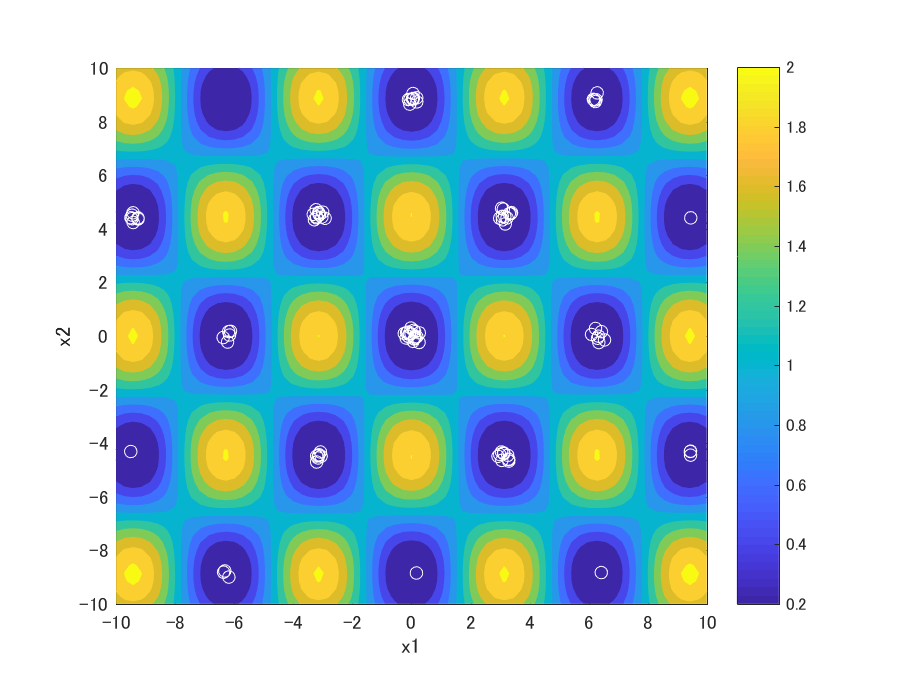
\includegraphics[width=0.8\linewidth]{eps/IES2018/f1_n100_1000.eps}
\label{fig:nsba-f1_n100_1000}}
\end{figure}

\begin{figure}[t]
\centering
\subfigure[$F_2 :(N=100)$]{
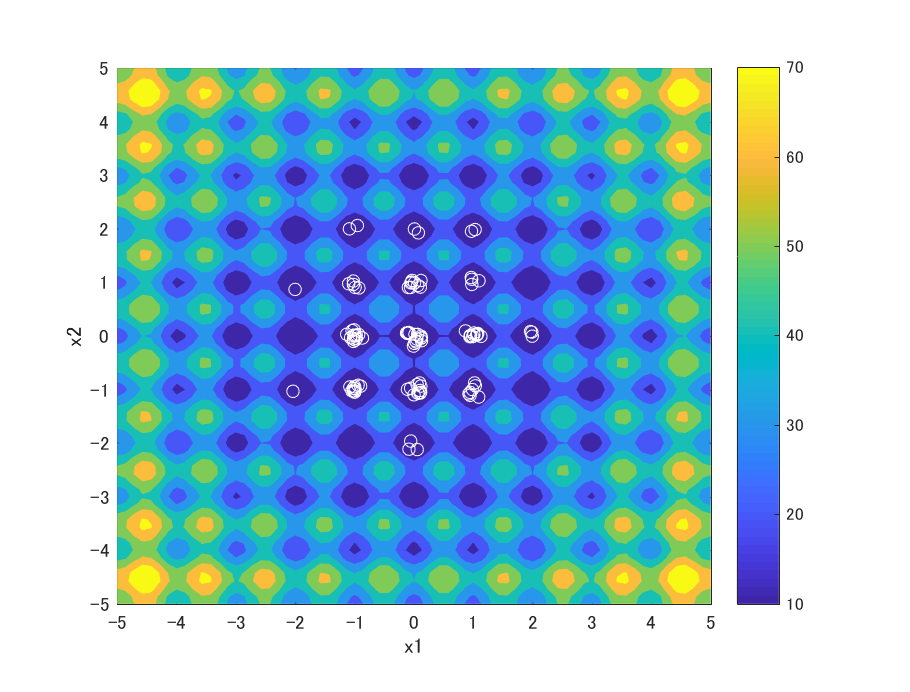
\includegraphics[width=0.8\linewidth]{eps/IES2018/f2_n100_1000.eps}
\label{fig:nsba-f2_n100_1000}}
\subfigure[$F_2 :(N=150)$]{
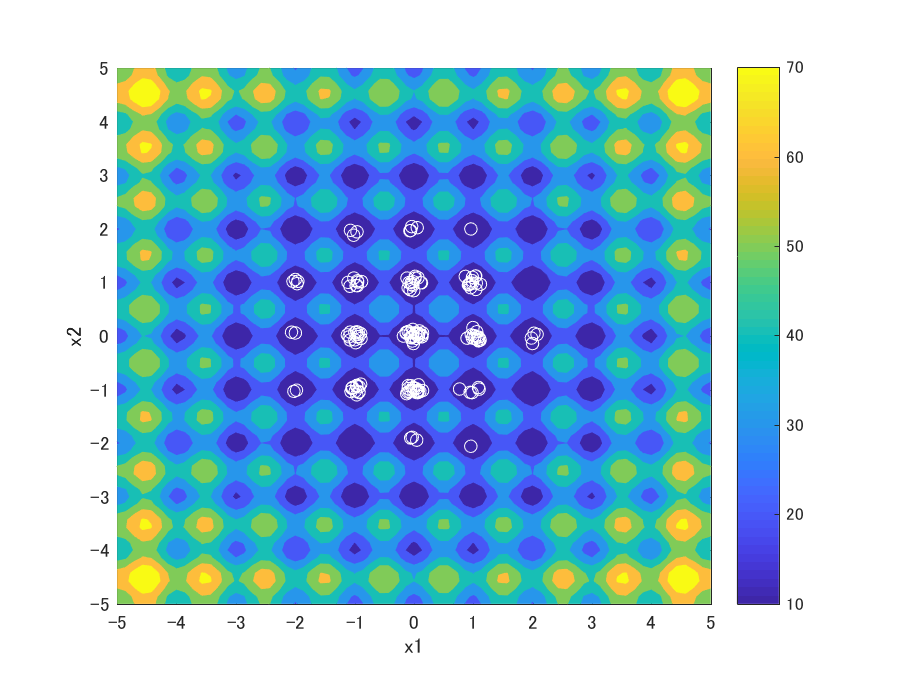
\includegraphics[width=0.8\linewidth]{eps/IES2018/f2_n150_1000.eps}
\label{fig:nsba-f2_n150_1000}}
\caption{Distribution of Solutions (NSBA)}
\label{fig:nsba-results_nsba_1000}
\end{figure}

\FloatBarrier
\newpage
\section{Niche Radius-based Bat Algorithm (NRBA)}
\label{sec:NRBA}
探索空間の分割方法の一つとしてNiche Radiusが挙げられる.Niche Radiusは探索空間のスケールと探索する解の数を元に個体の探索範囲を決定することのできる手法である.これにより,各個体が同じ解に留まることなく分散させ,従来のBAに以下3つの変更点を加えることで,最適解だけでなく局所解も同時に探索可能なNRBA \cite{NRBA} を説明する.

\subsection{メカニズム}
\label{ss:NRBA-abst}
従来手法のBAからの変更点を以下の図\ref{fig:nr_tab}に表し,その詳細を以下に示す.
\begin{figure}[h]
  \centering
  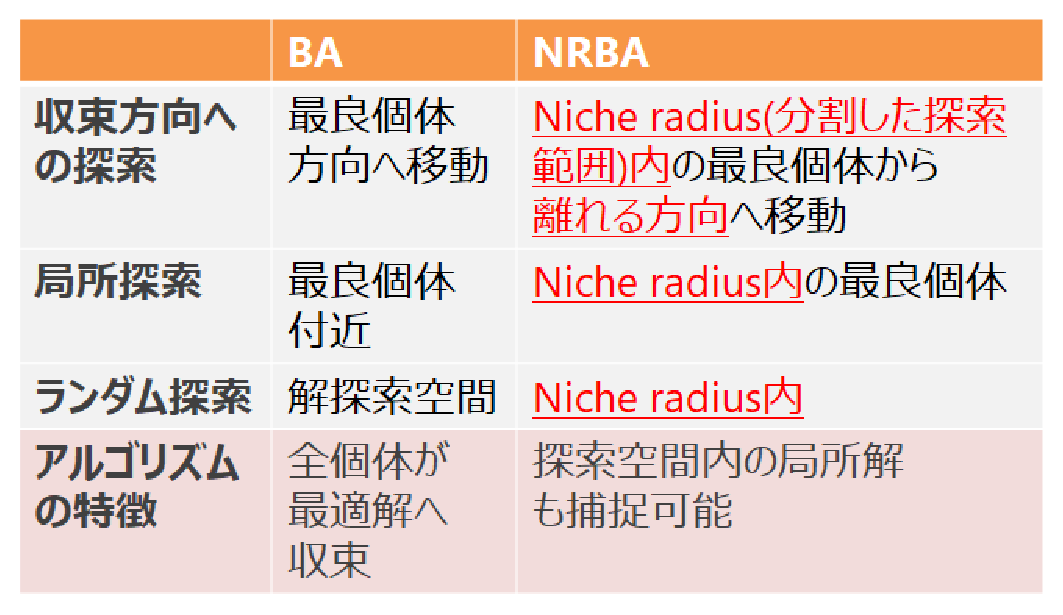
\includegraphics[width=0.7\linewidth]{eps/nr_table.eps}
  \caption{BAからの変更点}
  \label{fig:nr_tab}
\end{figure}

\begin{itemize}
\item {\bf BAからの変更点1:大域探索} \\
ここではNiche Radiusを使用し,従来であるBAの解候補の生成式(\ref{eq:ba-vi}),(\ref{eq:ba-xi})を次式のように変更を加えた.
\begin{equation}
\label{eq:nrvi}
\mbox{\boldmath $v_i^{t+1}$}=\mbox{\boldmath $v_i^t$}+(\mbox{\boldmath $x_i^t$}-\mbox{\boldmath $x_{NR*}$})*f_i
\end{equation}
\begin{equation}
\label{eq:nrxi}
\mbox{\boldmath $x_i^{t+1}$}= \begin{cases}
\mbox{\boldmath $x_i^t$}+\mbox{\boldmath $v_i^{t+1}$} & ({\rm if} \ d_i^t < \sigma) \\
\mbox{\boldmath $x_i^t$} & ({\rm otherwise})
\end{cases}
\end{equation}
個体移動時のイメージ図を図\ref{fig:nr}に表す.各個体はNRを半径とした円の探索領域が決まっており,個体間距離${d_i}$がNRより小さい場合において,式(\ref{eq:nrvi})にてNR内の最良解${x_{NR*}}$を中心とした円から離れる方向へ個体${x_i^t}$が速度${v_i}$で移動する.またNR内に他の個体が存在しない,あるいは最良解$x_{NR*}$は移動をせず,その場所に留まる.この変更により,個体が同じ探索領域内に留まらず分散化をはかる.
\begin{figure}[h]
  \centering
  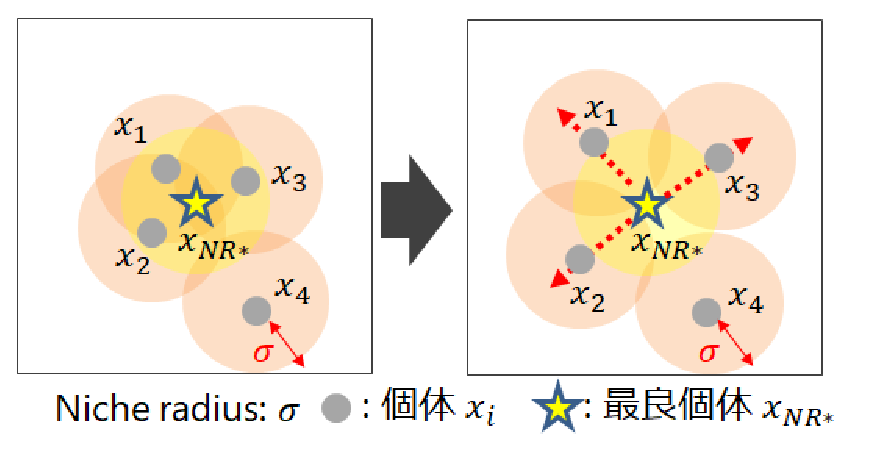
\includegraphics[width=0.7\linewidth]{eps/nr.eps}
  \caption{解候補の生成}
  \label{fig:nr}
\end{figure}

\item {\bf BAからの変更点2: 局所探索} \\
次に局所探索性能を上げるため,各個体が持つNiche Radius内の最良解${x_{NR*}}$の周辺に新しい解候補${x_{loc}}$を生成するよう変更した.生成式は次の通りである.
\begin{equation}
\label{eq:nrloc}
\mbox{\boldmath $x_{loc}$}=\mbox{\boldmath $x_{NR*}$} + \epsilon A_i^t
\end{equation}

$\epsilon$は1 $\times$ $D$次元の配列で$[-NR, \ NR]$区間のランダムな値が割り当てられる.この変更により,個体を局所解へ収束するよう促す.
\item {\bf BAからの変更点3: ランダム探索} \\
ランダム探索では各個体の持つNR内にランダムで解候補を以下の式のように生成する.
\begin{equation}
\label{eq:nrrnd}
\mbox{\boldmath $x_{rnd}$}=\mbox{\boldmath $x_i^t$} + rand(1,D,[-NR, NR])
\end{equation}
$[-NR, \ NR]$区間内の1×$D$次元の配列により現在位置$x_i^t$周辺に解候補を生成する.この変更では各個体を最適解あるいは局所解近辺へ移動させることで同じ場所に留まることを避ける.
\end{itemize}

\subsection{アルゴリズム}
\label{ss:NRBA-algorithm}
提案手法のNRBAのアルゴリズムの疑似コードをAlgorithm \ref{code:nrba}に記す.

\begin{itemize}
\item {\bf STEP1: 個体の初期化}\\
探索空間内にランダムに個体$x_i (i=1,2,...,N)$を生成し,周波数$f_i$,ラウドネス$A_i^0$,パルスレート$r_i^0$を決定する(1-3行目).
\item {\bf STEP2: 速度の更新と解候補の生成}\\
速度$v_i$により新しく解候補を生成する(7行目).
\item {\bf STEP3: 局所探索}\\
最良解$x_{pbest}$近辺に新しく解候補$x_{loc}$を生成する(10-11行目).
\item {\bf STEP4: ランダム探索}\\
探索空間内にランダムで解候補$x_{rnd}$を生成する(12行目).
\item {\bf STEP5: 評価と更新}\\
${\rm rand} < A_i$を満たす,かつ3つの解候補が$t$時点での最良解$x_{pbest}$よりも評価値が高ければ解を更新する(13-15行目).
\item {\bf STEP6: STEP2へ戻る}\\
終了条件を満たすまでSTEP2へ戻る.
\end{itemize}

\begin{algorithm}[H]
\caption{Niche Radius-based Bat Algorithm (NRBA)}
\label{code:nrba}
\begin{algorithmic}[2]
\REQUIRE Objective\ Function\ $F(x)$
\STATE Initialize Population $x_i(i=1,2,..., N)$ and $v_i$\\
\STATE Define frequency $f_i$ at location $x_i$ [eq.(\ref{eq:freq})]
\STATE Initialize pulse rates $r_i$, and loudness $A_i$
\WHILE{($t <$ Max number of iterations)}
\FOR{i=1 to N}
\IF{$d_{ij} < NR$}
\STATE Generate a new solution $x_i$ and velocity $v_i$ [Eqs.(\ref{eq:nrvi}) to (\ref{eq:nrxi})]
\ENDIF
\IF{($rand>r_i$)}
\STATE Generate a new solution $x_{loc}$ around personal best solution $x_{NR*}$ in Niche radius [Eq.(\ref{eq:nrloc})] 
% \ELSE
% \STATE Continue
\ENDIF
\STATE Generate a new solution $x_{rnd}$ randomly in Niche radius [Eq.(\ref{eq:nrrnd})]
\IF{($rand<A_i \& \min (F(x_i), F(x_{loc}), F(x_{rnd})<F(x_{i*})$)}
\STATE Accept the new solution, and update pulse rate $r_i$ \\ \& loudness $A_i$ [Eqs. (\ref{eq:loud})(\ref{eq:pulse})]  
\ENDIF
\STATE Evaluate all bats and select a best solution $x_*$ in the current solutions
\ENDFOR
\STATE t=t+1
\ENDWHILE
\end{algorithmic}
\end{algorithm}

\subsection{実験}
\label{ss:NRBA-exp}
最小化問題における最適解と局所解の数が異なる評価関数において,各手法の探索性能にどのような影響があるか調査する.次の4つのパターンの評価関数を用意し,従来手法であるBA,前章で提案したNSBAと比較することで提案手法の探索性能の有効性を検証する.一つの最適解に対して複数の局所解を持つ;複数の最適解に対して同じ数の局所解を持つ;一つの最適解の数に対して一つの局所解を持つ;最適解のみ複数持つ.これらのパターンに適した多峰性関数を用いて実験を行う.

\subsubsection{評価関数}
\label{sss:NRBA-func}
本実験で使用するベンチマーク関数は,\ref{ss:MinFunc}節で説明した$F_1$: Griewank,$F_3$: Six-Hump Camel,$F_4$: Michalewicz,$F_5$: Himmelblauの4つを用いる.

\subsubsection{評価基準}
\label{sss:NRBA-eval}
本実験において,Congress on Evolutionary Computation (CEC2013) \cite{CEC2013} のコンペティションで用いられた評価尺度であるPeak Ratio (PR) \cite{CDE} により評価する.評価式は以下のように設定した.
\begin{equation}
\label{eq:PR}
PR=\frac{\sum_{run=1}^{MR}FPs}{TP*MR}
\end{equation}
Max Run (MR) は実験回数を表し,Found Peaks (FPs) は発見した解の数を,Total Peak (TP) は探索領域内の全最適解及び局所解数を表す.また最適解及び局所解の位置座標と最近傍個体とのユークリッド距離が0.1未満であれば,その解を発見したと定義する.

\subsubsection{実験設定}
\label{sss:NRBA-setup}
個体数$N=50$とし,各個体のパラメータ$A_i^0=1$, $r_i^0 \in [0,\ 1]$,$f_{max}=1, f_{min}=0$, $\alpha = \gamma = 0.9$と設定した.またTable \ref{tab:minMOP}より,探索領域の上限$x_{ub}$と下限$x_{lb}$,各評価関数の解の総数$q$として使用した.また次元数$D=2$,世代数を10000,実験回数$MR=30$とした.

\subsubsection{実験結果}
\label{sss:NRBA-results}
各評価関数について,BAとNSBA,提案手法のNRBAにおけるPR値を表\ref{tab:nrba}に示す.表中のMean(平均値)とSD(標準偏差)は実験回数30回での最終世代における発見した最適解及び局所解数をPR値で表した結果である.各手法の最終世代での個体の分布を図 \ref{fig:results_ba}, \ref{fig:results_nrba}で表す.またグラフ中の赤い丸は個体の分布を示す.従来手法であるBAは全個体の最良解へ向かって進んでしまうため,全ての評価関数において,最適解あるいは評価値の高い局所解に収束した.しかし図\ref{fig:nrba-f4_ba}については局所解は存在しないが,最終世代では一つの最適解へ収束する結果となった.NSBAは全ての評価関数に対してBAよりもPR値が高く,特に局所解を含まない$F_5$関数においては全ての最適解を探索することが可能であった.一方で提案したNRBAは図\ref{fig:results_nrba}から全評価関数において,全ての解に個体が到達しているように分布しているが,表\ref{tab:nrba}から全体的にBAやNSBAよりも探索性能が高かったが,最適解や局所解の位置まで到達していないケースが多く見られた.また最適解や局所解に到達していない個体については用いた評価関数によって分布に偏りがあった.

\begin{figure}[t]
\centering
\subfigure[$F_1$: Griewank]{
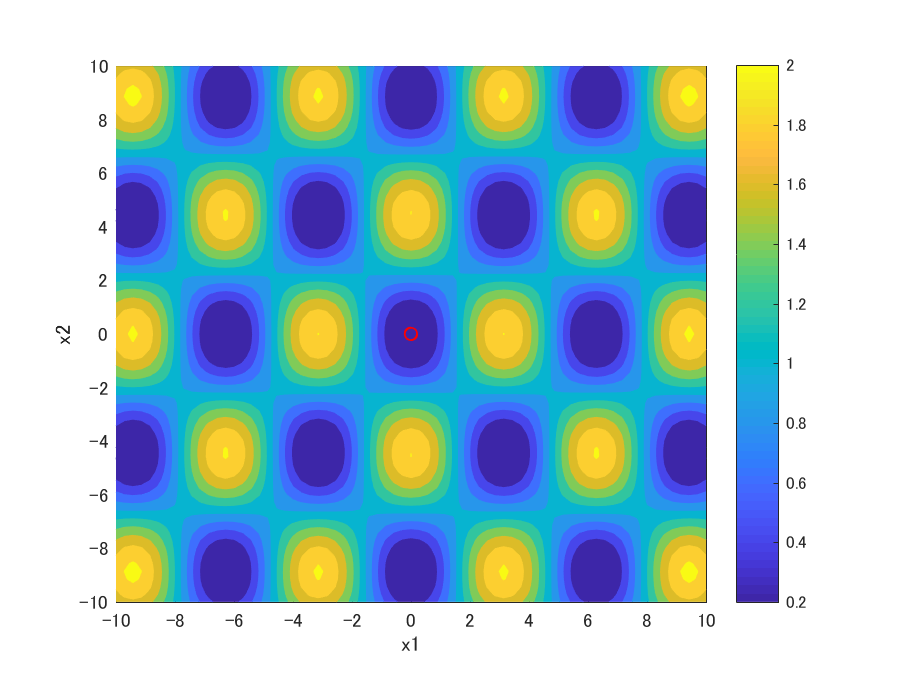
\includegraphics[width=0.9\linewidth]{eps/SICESSI2018/f1_ba.eps}
\label{fig:nrba-f1_ba}}
\subfigure[$F_3$: Six-Hump Camel]{
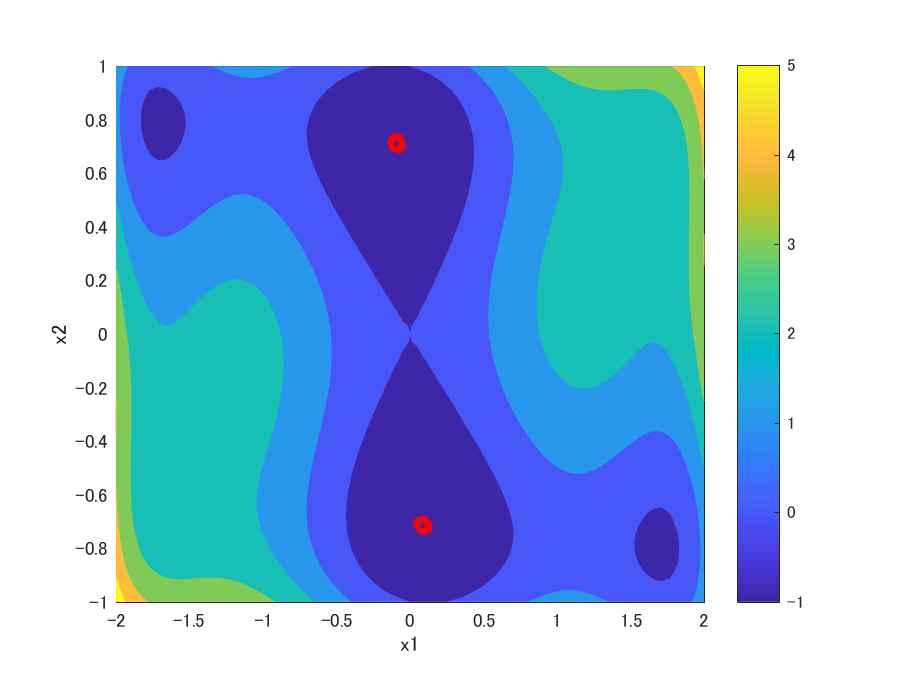
\includegraphics[width=0.9\linewidth]{eps/SICESSI2018/f2_ba.eps}
\label{fig:nrba-f2_ba}}
\end{figure}

\begin{figure}[h]
\centering
\subfigure[$F_4$: Michalewicz]{
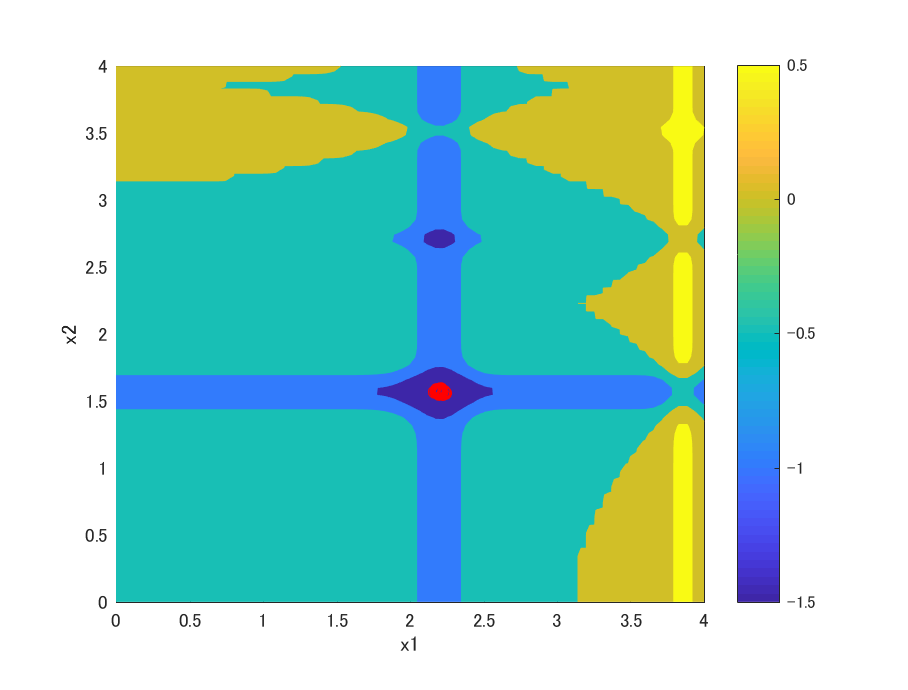
\includegraphics[width=0.9\linewidth]{eps/SICESSI2018/f3_ba.eps}
\label{fig:nrba-f3_ba}}
\subfigure[$F_5$: Himmelblau]{
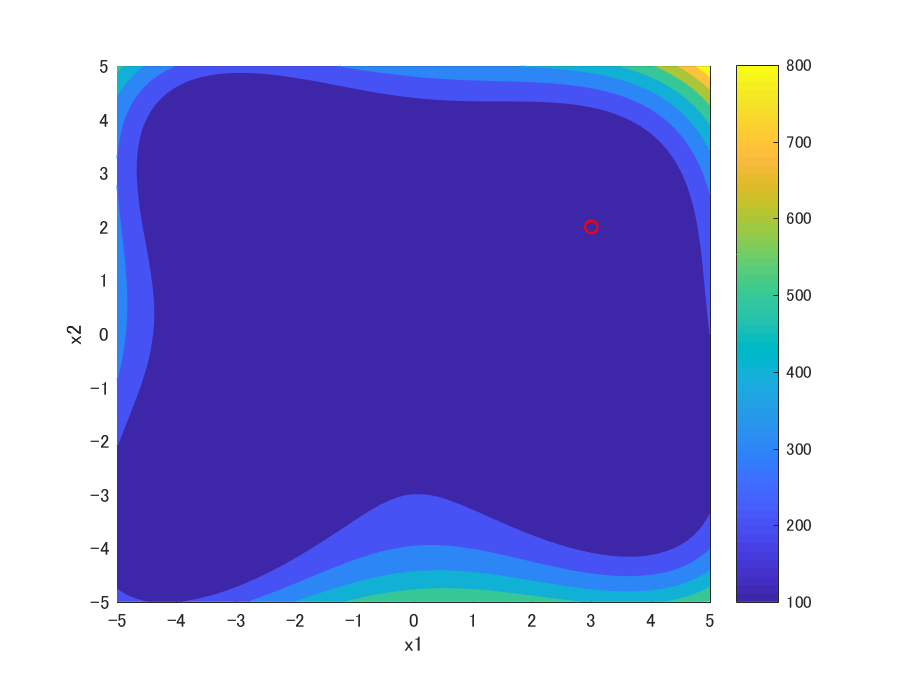
\includegraphics[width=0.9\linewidth]{eps/SICESSI2018/f4_ba.eps}
\label{fig:nrba-f4_ba}}
\caption{BA}
\label{fig:results_ba}
\end{figure}


\begin{figure}[h]
\centering
\subfigure[$F_1$: Griewank]{
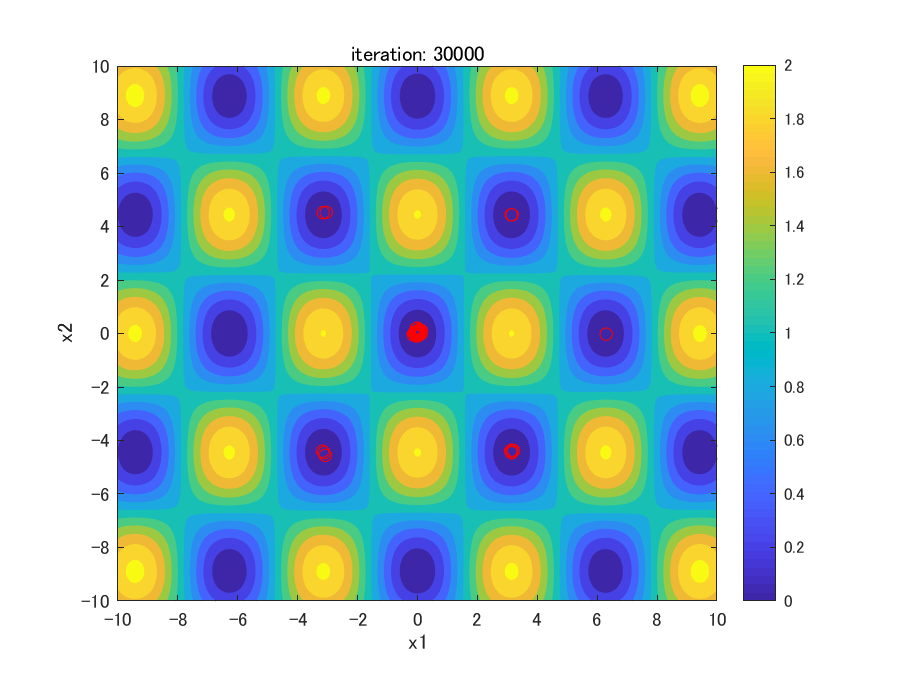
\includegraphics[width=0.9\linewidth]{eps/SICESSI2018/f1_nsba.eps}
\label{fig:nrba-f1_nsba}}
\subfigure[$F_3$: Six-Hump Camel]{
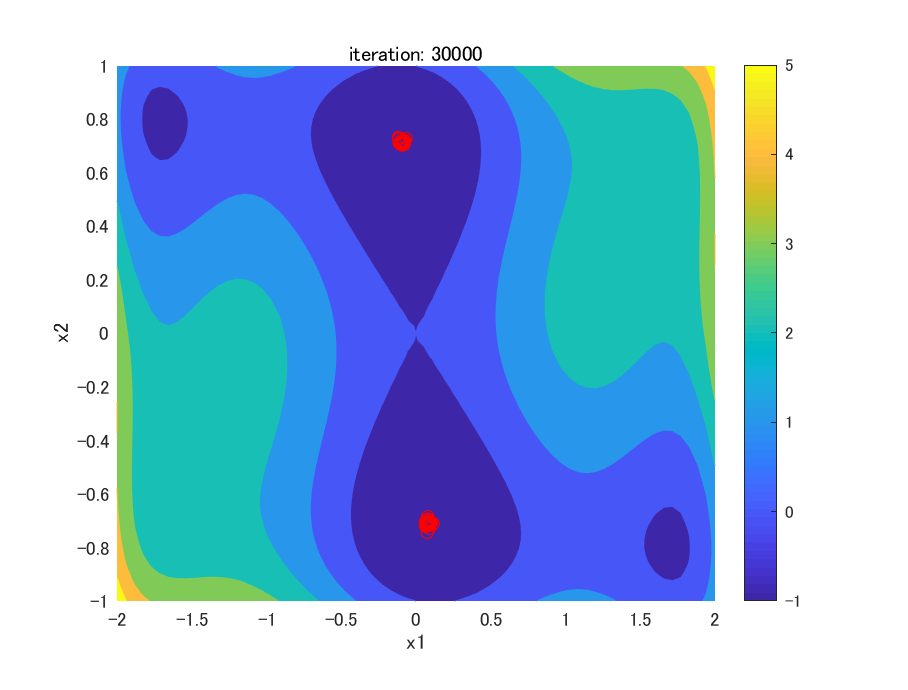
\includegraphics[width=0.9\linewidth]{eps/SICESSI2018/f2_nsba.eps}
\label{fig:nrba-f2_nsba}}
\end{figure}

\begin{figure}[h]
\centering
\subfigure[$F_4$: Michalewicz]{
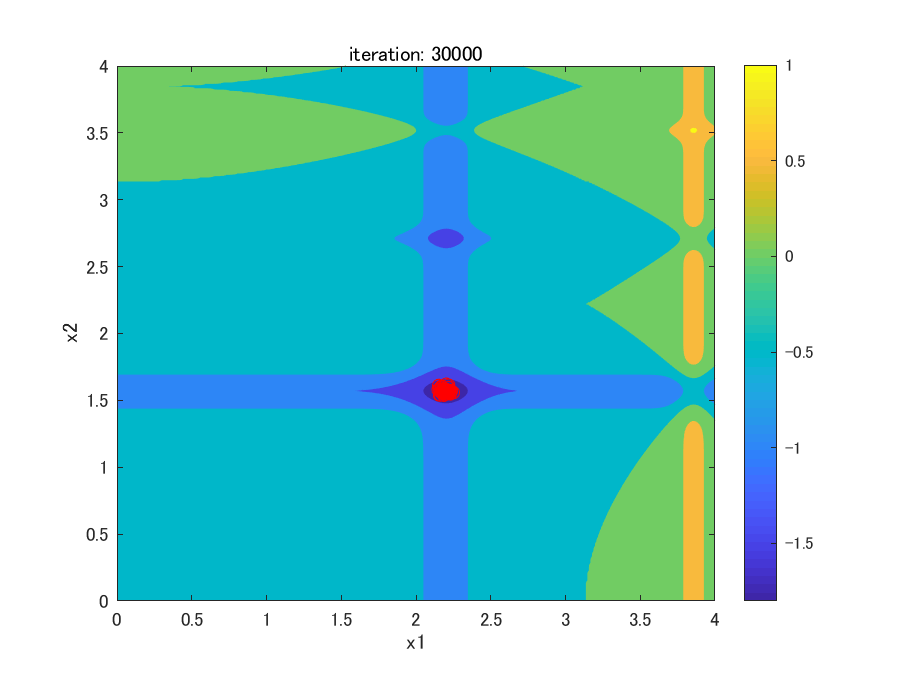
\includegraphics[width=0.9\linewidth]{eps/SICESSI2018/f3_nsba.eps}
\label{fig:nrba-f3_nsba}}
\subfigure[$F_5$: Himmelblau]{
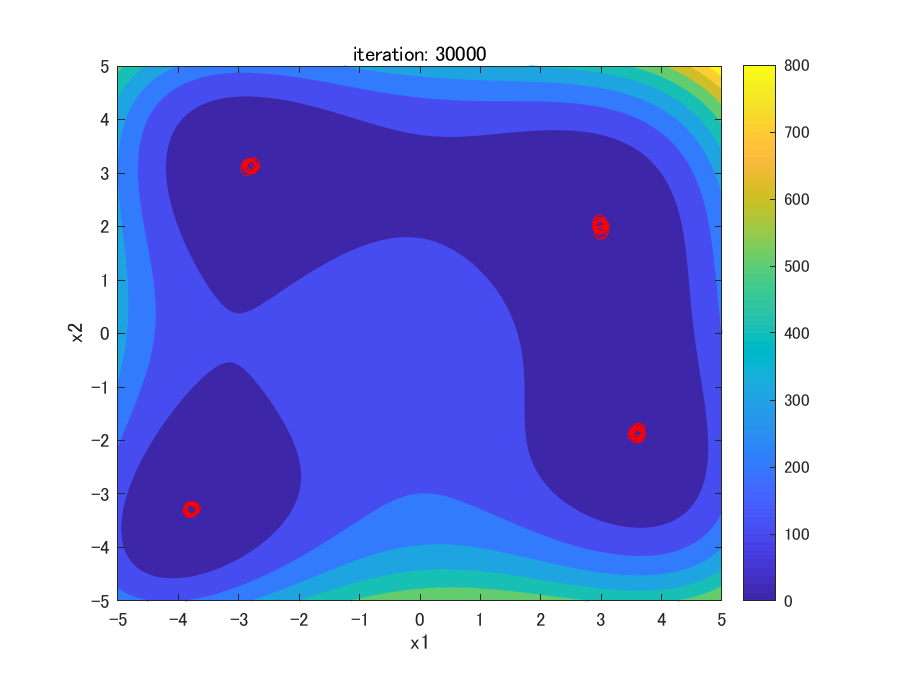
\includegraphics[width=0.9\linewidth]{eps/SICESSI2018/f4_nsba.eps}
\label{fig:nrba-f4_nsba}}
\caption{NSBA}
\label{fig:results_nsba}
\end{figure}


\begin{figure}[h]
\centering
\subfigure[$F_1$: Griewank]{
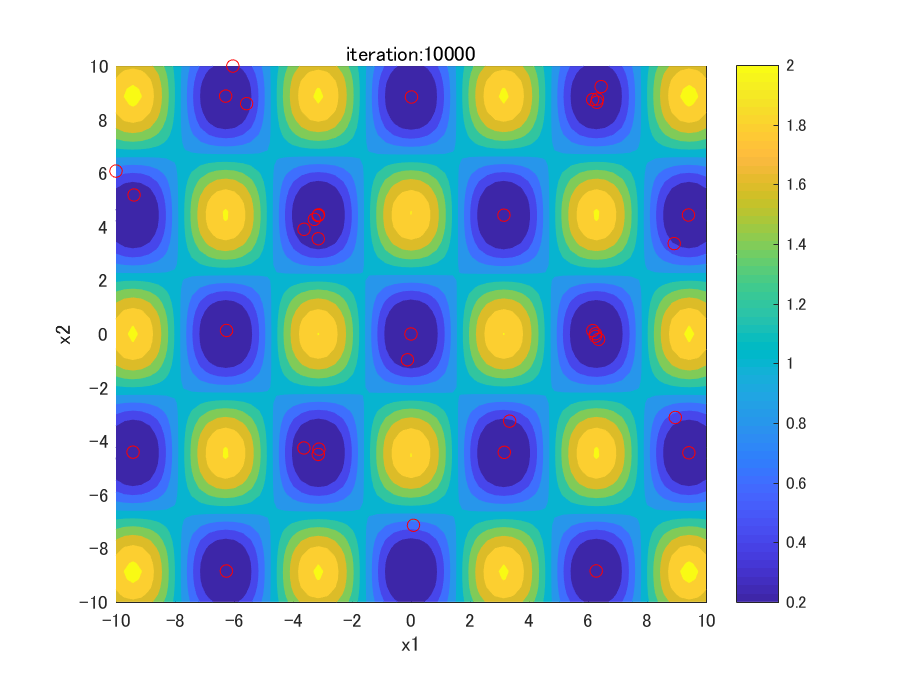
\includegraphics[width=0.9\linewidth]{eps/SICESSI2018/f1_nrba.eps}
\label{fig:nrba-f1_nrba}}
\subfigure[$F_3$: Six-Hump Camel]{
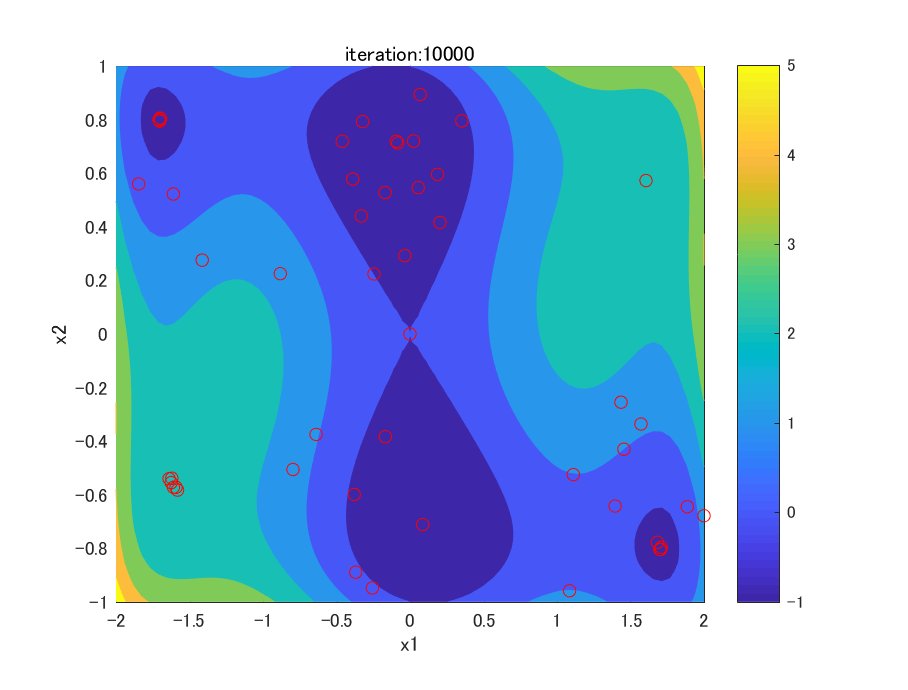
\includegraphics[width=0.9\linewidth]{eps/SICESSI2018/f2_nrba.eps}
\label{fig:nrba-f2_nrba}}
\end{figure}

\begin{figure}[h]
\centering
\subfigure[$F_4$: Michalewicz]{
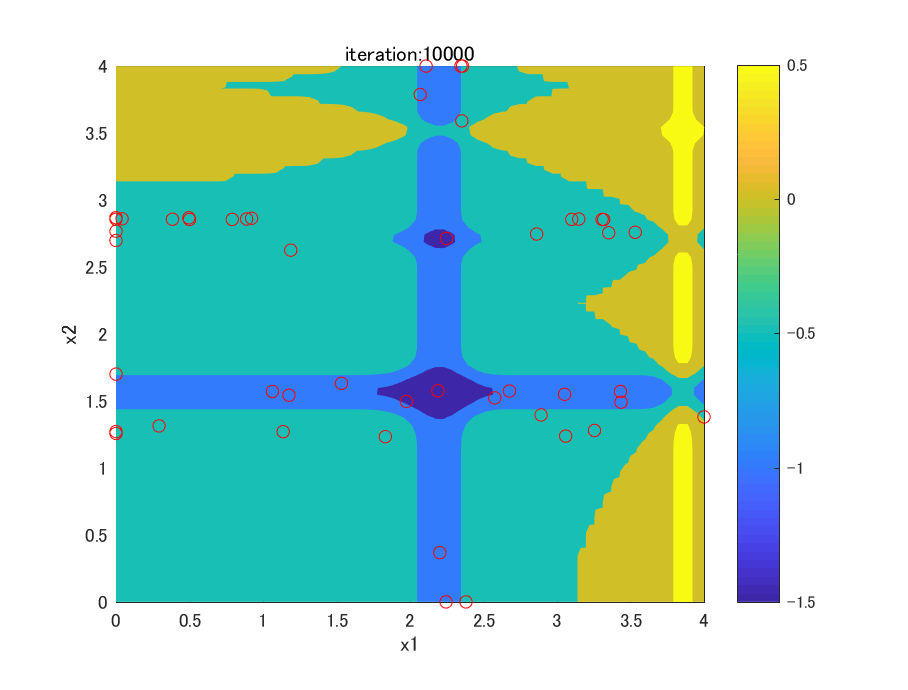
\includegraphics[width=0.9\linewidth]{eps/SICESSI2018/f3_nrba.eps}
\label{fig:nrba-f3_nrba}}
\subfigure[$F_5$: Himmelblau]{
\includegraphics[width=0.9\linewidth]{eps/SICESSI2018/f4_nrba.eps}
\label{fig:nrba-f4_nrba}}
\caption{NRBA}
\label{fig:results_nrba}
\end{figure}

\begin{table}[h]
\caption{The value of PR (averaged over 30 runs)}
\begin{center}
\begin{tabular}{c|c|c|c}
\hline
\multicolumn{1}{c|}{} & \multicolumn{1}{c|}{BA} & \multicolumn{1}{c|}{NSBA} & \multicolumn{1}{c}{NRBA}  \\
\hline
Function & Mean $\pm$ SD  & Mean $\pm$ SD &  Mean $\pm$ SD \\
\hline
$F_1$ & 0.0588 $\pm$ 0 & 0.3760 $\pm$ 0.0413 & {\bf 0.6922} $\pm$ 0.0981  \\
\hline
$F_3$ & 0.4917 $\pm$ 0.0449 & 0.5 $\pm$ 0 & {\bf 0.9917} $\pm$ 0.0449 \\
\hline
$F_4$ & 0.5 $\pm$ 0 & 0.5 $\pm$ 0 & {\bf 0.7} $\pm$ 0.2450 \\
\hline
$F_5$ & 0.2417 $\pm$ 0.1367 & {\bf 1} $\pm$ 0 & 0.8583 $\pm$ 0.1239 \\
\hline
\end{tabular}
\label{tab:nrba}
\end{center}
\end{table}

\subsection{考察}
\label{ss:nrba-disc}
全体的に,BAやNSBAより提案のNRBAのほうが探索した解の数および発見率が高かったことから最適解への収束を防ぎ,複数の局所解へ分散させることができた.また提案手法の探索性能の有効性を確かめるため,評価尺度による解の発見数及び発見率の結果と,最終世代の解の分布という観点から分析を行った.


\subsubsection{解の発見数}
\label{sss:nrba-pr} 
表\ref{tab:nrba}から従来手法のBAは全ての評価関数において一つの解へ収束する傾向が強かったが,$F_2$関数では2つの解を探索することができた.これは従来手法のアルゴリズムの解候補の生成において,全個体の最良解へ向かって探索をしていることが原因であると考えられる.NSBAについても同様,収束性能が高いために,同じ局所解に複数の個体が密集していることが確認できたが,$F_4$関数においては全ての最適解に到達することが可能であった.これは,最適解の評価値が全て均一であったため,結果として一つの最適解に留まらなかったと考えられる.提案手法のNRBAは全ての評価関数に対して,従来手法よりも発見した解の数が多く,最適解と複数の局所解を探索することができた.評価関数の中でも$F_2$関数,次いで$F_4$関数のPRの値が高いことから最適解のみ存在する場合と,最適解と局所解の評価値の差が小さい場合において提案手法の探索が有効に働いたと考えられる.また局所解を多く含む$F_1$関数や局所解の範囲が非常に狭い$F_3$関数では探索性能が落ちたことから今後の課題として手法を改良する必要がある.

\subsubsection{最終世代における解の分布}
\label{sss:dstr_sol} 
図\ref{fig:results_ba}から従来のBAは,最適解への収束が非常に強かった.しかし,図\ref{fig:nrba-f2_ba}では2つの最適解に収束していたものの,図\ref{fig:nrba-f4_ba}では複数の最適解へ収束することなく一つの最適解へ収束した.これは,$F_4$関数の方が探索領域が広く,評価値の数値の範囲も広いことから各個体の持つ評価値にバラつきが出やすく,一つの最適解へ収束したと考えられる.図\ref{fig:results_nrba}より提案手法のNRBAは,図\ref{fig:nrba-f1_nrba}では色濃度の濃い領域に各個体を分散させることができたが,図\ref{fig:nrba-f2_nrba}, \ref{fig:nrba-f3_nrba}, \ref{fig:nrba-f4_nrba}では最適解や局所解でない場所に分布する個体も多く見られた.このことから従来手法から変更した,Niche Radius内の最良解より個体が遠ざかる機構が働いたと考えられる.以上より探索領域を分割し,各個体の探索領域内での大域探索性能を保ちながらも徐々に局所解へ収束させることが,解の発見率の増加に繋がったと考えられる.


\clearpage
\newpage
\section{Dynamic Niche Radius-based Bat Algorithm (DNRBA)}
\label{sec:DNRBA}
本章では,NRBAで局所解に収束しなかった個体を最適解や局所解へ移動させることで,収束性能を高めることを目的としたDynamic Niche RadiusをBAに適用させたDNRBAを提案する.
\subsection{メカニズム}
\label{ss:DNRBA-abst}
\ref{ss:dns}節で説明したDynamic Niche Sharing \cite{DNS} より,探索領域に属する個体が同じ局所解に収束することを避けるため,本研究では以下の変更を加えた.
\begin{equation}
\label{eq:mi}
m_i^{dyn}=\begin{cases}
\sigma & ({\rm if } \ m_i < \sigma) \\
m_i & ({\rm otherwise})
\end{cases}
\end{equation}

\begin{equation}
\label{eq:dnrba-vi}
 \mbox{\boldmath $v_i^{t+1}$} = \mbox{\boldmath $v_i^t$} + (\mbox{\boldmath $x_i^t$}-\mbox{\boldmath $x_{NR*}$})*f_i
\end{equation}
$v_i$,$x_i$は個体の速度と位置を表し,$x_{NR*}$は$x_i$が属するNiche Radius内の最良個体を示す.
(\ref{eq:mi})式に基づいて,個体の更新式は以下で表される.
\begin{equation}
\label{eq:dnrba-xi}
\mbox{\boldmath $x_i^{t+1}$}=\begin{cases}
\mbox{\boldmath $x_i^t$}+\mbox{\boldmath $v_i^{t+1}$} & ({\rm if} \ m_i < \sigma) \\
\mbox{\boldmath $x_i^t$} & ({\rm otherwise})
\end{cases}
\end{equation}
ここでは個体の分布密度が高いほど,個体$x_i$の持つNiche Count $m_i$の範囲内にある最良個体$x_{NR*}$から遠ざかる方向へ新たに解候補を生成する.探索範囲決定のイメージ図\ref{fig:dnr}に示す.

\begin{figure}[h]
\centering
\includegraphics[width=0.7\linewidth]{eps/dynamic_niche_radius.eps}
\label{fig:dnr}
\caption{Dynamic Niche Radiusのイメージ図}
\end{figure}

局所探索では(\ref{eq:mi})式で算出した最良個体$x_{NR*}$が持つ$m_i$の範囲内で個体$x_i$が新たに解候補$x_{loc}$を生成する.
\begin{equation}
\label{eq:dnrloc}
\mbox{\boldmath $x_{loc}$}=\mbox{\boldmath $x_{NR*}$} + A_i^t*rand(1,D,[-m_i, m_i])
\end{equation}
ランダム探索では,個体$x_i$の持つ$m_i$の範囲内で新たに解候補$x_{rnd}$を生成することで,局所解への収束性能を高める.生成式は次式で表される.
\begin{equation}
\label{eq:dnrrnd}
\mbox{\boldmath $x_{rnd}$}=\mbox{\boldmath $x_i^t$} + rand(1,D,[-m_i, m_i])
\end{equation}

\subsection{アルゴリズム}
\label{sss:DNRBA-algorithm}
DNRBAのアルゴリズムの疑似コードを以下のAlgorithm \ref{code:dnr}, \ref{code:dnrba}に記す.

\begin{itemize}
\item {\bf STEP1: 個体の初期化}\\
探索空間内にランダムに個体$x_i (i=1,2,...,N)$を生成し,周波数$f_i$,ラウドネス$A_i^0$,パルスレート$r_i^0$を決定する(1-3行目).
\item {\bf STEP2: Dynamic Niche Radius算出}\\
Algorithm \ref{code:dnr}により,各個体の持つniche count $m_i$を算出する(5行目).
\item {\bf STEP3: 速度の更新と解候補の生成}\\
速度$v_i$により新しく解候補を生成する(8行目).
\item {\bf STEP4: 局所探索}\\
最良解$x_{pbest}$近辺に新しく解候補$x_{loc}$を生成する(10-11行目).
\item {\bf STEP5: ランダム探索}\\
探索空間内にランダムで解候補$x_{rnd}$を生成する(13行目).
\item {\bf STEP6: 評価と更新}\\
${\rm rand} < A_i$を満たす,かつ3つの解候補が$t$時点での最良解$x_{pbest}$よりも評価値が高ければ解を更新する(14-16行目).
\item {\bf STEP6: STEP2へ戻る}\\
終了条件を満たすまでSTEP2へ戻る.
\end{itemize}

\begin{algorithm}[h]
\caption{Dynamic Niche Radius}
\label{code:dnr}
\begin{algorithmic}[2]
\REQUIRE Current Population $x_i(i=1,2,..., N)$ and $v_i$
\FOR{i=1 to N}
\FOR{j=1 to N}
\STATE Calculate $d_{ij}$ between individuals $i,j$
\IF{( $d_{ij} < \sigma$)}
\STATE $sh(d_{ij}) =  (1-\frac{d_{ij}}{\sigma})$ [Eq.(\ref{eq:sfunc})]
\ELSE
\STATE $sh(d_{ij}) =  0 $ [Eq.(\ref{eq:sfunc})]
\ENDIF
\ENDFOR
\STATE $m_i=\sum_{j=1}^N sh(d_{ij})$ [Eq.(\ref{eq:nc})]
\ENDFOR
\FOR{i=1 to N}
\IF{$(m_i < \sigma)$}
\STATE $m_i^{dyn}=\sigma$ [Eq.(\ref{eq:mi})]
\ELSE 
\STATE $m_i^{dyn} = m_i$ [Eq.(\ref{eq:mi})]
\ENDIF
\ENDFOR
\RETURN Dynamic Niche Radius $m_i^{dyn}$
\end{algorithmic}
\end{algorithm}

\begin{algorithm}[h]
\caption{Bat Algorithm with Dynamic Niche Radius (DNRBA)}
\label{code:dnrba}
\begin{algorithmic}[3]
\REQUIRE Objective\ Function\ $F(x)$
\STATE Initialize Population $x_i(i=1,2,..., N)$ and $v_i$\\
\STATE Define frequency $f_i$ at location $x_i$ [Eq.(\ref{eq:freq})]
\STATE Initialize pulse rates $r_i$, and loudness $A_i$
\WHILE{($t <$ Max number of iterations)}
\STATE Calculate Dynamic Niche Radius (Algorithm 2)
\FOR{i=1 to N}
\IF{$d_{ij} < NR$}
\STATE Generate a new solution $x_i$ and velocity $v_i$ [Eqs.(\ref{eq:dnrba-vi}) and (\ref{eq:dnrba-xi})]
\ENDIF
\IF{($rand>r_i$)}
\STATE Generate a new solution $x_{loc}$ around personal best solution $x_{NR*}$ in Niche radius [Eq.(\ref{eq:dnrloc})] 
% \ELSE
% \STATE Continue
\ENDIF
\STATE Generate a new solution $x_{rnd}$ randomly in Niche radius [Eq.(\ref{eq:dnrrnd})]
\IF{($rand<A_i \& \min (F(x_i), F(x_{loc}), F(x_{rnd})<F(x_{i*})$)}
\STATE Accept the new solution, and update pulse rate $r_i$ \\ \& loudness $A_i$ [Eqs. (\ref{eq:loud}) and (\ref{eq:pulse})]  
\ENDIF
\STATE Evaluate all bats and select a best solution $x_*$ in the current solutions
\ENDFOR
\ENDWHILE
\end{algorithmic}
\end{algorithm}

\subsection{実験}
\label{ss:DNRBA-exp}
DNRBAの収束性能を検証するため,ここではBAと比較する.本実験では最小化問題における,最適解と局所解を持つGriewank関数とShubert関数を用いた.

\subsubsection{評価関数}
\label{sss:DNRBA-func}
本実験では,評価関数は\ref{ss:MinFunc}節で説明した$F_1$, $F_6$関数を使用する.

% \begin{description}
% \item[$F_1$: Griewank Function]\mbox{}\\
% Griewank関数の概形を図\ref{fig:dnrba-f1}に示す.
% \begin{equation}
% F_1(x)= \sum_{i=1}^D \frac{x_{i}}{4000} - \prod_{i=1}^D \cos(\frac{x_i}{\sqrt{i}}) + 1,
% \label{eq:dnrba-f1}
% \end{equation}
% 最適解の評価値は${F(x_*)}=0$であり,1つの最適解と16個の局所解を持つ.探索範囲は$x_1, x_2 \in [-10, \ 10]$である.

% % \begin{figure}[h]
% % \centering
% % \subfigure[Fitness landscape]{
% % \includegraphics[width=0.8\linewidth]{eps/ISMSI2019/3d_griewank.eps}
% % \label{fig:3df1}}
% % \subfigure[Contour plot]{
% % \includegraphics[width=0.8\linewidth]{eps/ISMSI2019/cont_griewank.eps}
% % \label{fig:cf1}}

% % \caption{$F_1$: Griewank Function}
% % \label{fig:dnrba-f1}
% % \end{figure}

% \item[$F_2$: Shubert Function]\mbox{}\\
% Shubert関数の概形を図\ref{fig:dnrba-f2}に示す.
%  \begin{equation}
% F_2(x) = \prod_{i=1}^D \sum_{j=1}^5 j \cos[(j+1)x_i+j], 
% \end{equation}
% $D$は次元数を表し,最適解の評価値は${F(x_*)=-187.731}$である.この関数では$D \cdot 3^D $個の最適解のみ存在し,2次元では18個の最適解を持つ.探索範囲は$x_i \in [-10, 10]^D$ $(i=1,2,...,D)$である.

% \begin{figure}[h]
% \centering
% \subfigure[Fitness landscape]{
% \includegraphics[width=0.8\linewidth]{eps/ISMSI2019/3d_shubert.eps}
% \label{fig:3df2}}
% \subfigure[Contour plot]{
% \includegraphics[width=0.8\linewidth]{eps/ISMSI2019/cont_shubert.eps}
% \label{fig:cf2}}

% \caption{$F_2$: Shubert Function}
% \label{fig:dnrba-f2}
% \end{figure}

% \end{description}


\subsubsection{評価基準}
\label{sss:DNRBA-eval}

\subsubsection{Peak Ratio}
本実験ではCEC2013 Competitionで用いられたPeak Ratio (PR) \cite{CEC2013} を用い,発見した解の数の割合を求める.PRの算出式は次式で表される.
\begin{equation}
PR=\frac{\sum_{run=1}^{MR}FPs}{TP*MR}
\end{equation}
Max Run (MR) は実験回数を表し,Found Peaks (FPs) は発見した解の数を,Total Peak (TP) は探索領域内の全最適解及び局所解数を表す.また最適解及び局所解の位置座標と最近傍個体とのユークリッド距離が0.1未満であれば,その解を発見したと定義する.

\subsubsection{Peak Accuracy}
探索する個体が最適解にどのくらい近づいているかを計測する尺度としてPeak Accuracy (PA) \cite{CEC2013} を用いる.PAの算出式は以下で表される.
\begin{equation}
PA=\sum_{j=1}^{TP}|F(s_j)-F(x_{NN_j})|,
\end{equation}
この時,$F(s_j)$は$j$番目の最適解の評価値を表し,その最近傍個体$x_{NN_j}$の評価値との差分和を求める.則ち,PA値が0に近づくほど,個体が最適解に位置していることを示す.

\FloatBarrier
\subsection{実験設定}
本実験では$f_{max}=1$, $f_{min}=0$,ラウドネス$A^0=1$,パルスレート$r^0 \in [0,1]$と設定した.また$\alpha= \gamma = 0.9$とし,個体数を100,世代数を30000としてランダムシードを変えた実験を30回行った.

\subsection{実験結果と考察}
\label{sss:DNRBA-results}
本節ではDNRBAの性能の効果を確かめるため,各評価関数におけるPRとPAに着目する.表\ref{tab:dnrba-1}, \ref{tab:dnrba-2}は,BAとDNRBAのアルゴリズムにおけるPRとPAの結果を表す.各評価関数のPRとPAの30試行の平均値及び標準偏差を示している.また図\ref{fig:dnrba-results_ba},\ref{fig:dnrba-results_dnrba}は最終世代の個体の分布を白い丸で表す.

\begin{table}[h]
\caption{PR and PA of BA and DNRBA (averaged over 30 runs)}
\begin{center}
\begin{tabular}{c|c|c|c|c}
\multicolumn{5}{c}{$\varepsilon = 1.0E-1$} \\
\hline
\multicolumn{1}{c|}{} & \multicolumn{2}{c|}{BA} & \multicolumn{2}{c}{DNRBA} \\
\hline
 & PR & PA & PR & PA \\

Function & (Mean and SD) & (Mean and SD) & (Mean and SD) & (Mean and SD) \\
\hline
$F_1 $ & 0.2725 $\pm$ 0.0598 & 0.2416 $\pm$ 0.0149 & {\bf 0.9373} $\pm$ 0.1176  & {\bf 0.0094} $\pm$ 0.0155  \\
\hline
$F_6 $ & {\bf 0.4889} $\pm$ 0.1819 & {\bf 1.8160} $\pm$ 0.4990 & 0.4241 $\pm$ 0.388 & 2.4123 $\pm$ 0.6780 \\
\hline

\end{tabular}
\label{tab:dnrba-1}
\end{center}
\end{table}

\begin{table}[h]
\caption{PR and PA of BA and DNRBA (averaged over 30 runs)}
\begin{center}
\begin{tabular}{c|c|c|c|c}
\multicolumn{5}{c}{$\varepsilon = 1.0E-2$} \\
\hline
\multicolumn{1}{c|}{} & \multicolumn{2}{c|}{BA} & \multicolumn{2}{c}{DNRBA} \\
\hline
 & PR & PA & PR & PA \\

Function & (Mean and SD) & (Mean and SD) & (Mean and SD) & (Mean and SD) \\
\hline
$F_1 $ & 0.2725 $\pm$ 0.0608 & 0.2416 $\pm$ 0.0151 & {\bf 0.9373} $\pm$ 0.1176  & {\bf 0.0094} $\pm$ 0.0155  \\
\hline
$F_6 $ & {\bf 0.0556} $\pm$ 0.0619 & {\bf 1.8160} $\pm$ 0.4990 & 0.0426 $\pm$ 0.0477 & 2.4123 $\pm$ 0.6780 \\
\hline

\end{tabular}
\label{tab:dnrba-2}
\end{center}
\end{table}

\subsubsection{Peak Ratio}
表\ref{tab:dnrba-1}より$\varepsilon=1.0E-1$の$F_1$関数では,BAよりもDNRBAのPR値の方が高く,図\ref{fig:dnrba-f1dnrba}からほぼ全ての最適解と局所解を発見していることが分かる.対して$F_6$関数では,図\ref{fig:dnrba-f2ba},\ref{fig:dnrba-f2dnrba}から個体が全最適解に位置しているように見て取れるが,DNRBAよりもBAの方が僅かにPR値が高かった.このことから最適解しか存在しない関数についてはBAのほうが探索性能則ち収束性能が高いことが分かった.$\varepsilon=1.0E-2$についても同様,PR値は$F_1$関数はDNRBAの方が高く,$F_6$関数ではBAの方が高かった.

\subsubsection{Peak Accuracy}
表\ref{tab:dnrba-1}, \ref{tab:dnrba-2}から$F_1$関数では,BAよりDNRBAの方がPA値が高かったが,$F_6$関数ではBAの方がPA値が高かった.これは,従来BAの収束する方向へ解候補を生成する機構が働いていることが一つの要因として考えられる.加えてランダム探索において,探索空間内に解候補を生成することでPA値がより良くなったと考えられる.

\begin{figure}[h]
\centering
\subfigure[$F_1$]{
\includegraphics[width=0.8\linewidth]{eps/ISMSI2019/f1_ba.eps}
\label{fig:dnrba-f1ba}}
\subfigure[$F_6$]{
\includegraphics[width=0.8\linewidth]{eps/ISMSI2019/f2_ba.eps}
\label{fig:dnrba-f2ba}}

\caption{BA}
\label{fig:dnrba-results_ba}
\end{figure}

\begin{figure}[h]
\centering
\subfigure[$F_1$]{
\includegraphics[width=0.8\linewidth]{eps/ISMSI2019/f1_nrba.eps}
\label{fig:dnrba-f1nrba}}
\subfigure[$F_6$]{
\includegraphics[width=0.8\linewidth]{eps/ISMSI2019/f2_nrba.eps}
\label{fig:dnrba-f2nrba}}

\caption{NRBA}
\label{fig:dnrba-results_nrba}
\end{figure}

\begin{figure}[t]
\centering
\subfigure[$F_1$]{
\includegraphics[width=0.8\linewidth]{eps/ISMSI2019/f1_dnrba.eps}
\label{fig:dnrba-f1dnrba}}
\subfigure[$F_6$]{
\includegraphics[width=0.8\linewidth]{eps/ISMSI2019/f2_dnrba.eps}
\label{fig:dnrba-f2dnrba}}

\caption{DNRBA}
\label{fig:dnrba-results_dnrba}
\end{figure}

% \subsection{まとめ}

\FloatBarrier
\newpage
\section{他の最先端手法との性能比較実験}
\label{sec:experiment}


% \subsection{複数解探索における多峰性最適化問題}
% \label{ss:cec2013}
% 本実験では,複数最適解を探索する手法の性能を比較するため,CEC ({\it IEEE Congress on Evolutionary Computation}) 2013 Competition on Niching Methods for Multimodal Function Optimization \cite{CEC2013} で扱われたベンチマーク関数を用いる.使用する関数について,次節で説明する.

\subsection{評価関数}
\label{sss:benchmark}
使用するベンチマーク関数とその概形は\ref{ss:maxFunc}節で説明した6つの評価関数を用いる.


\subsection{評価基準}
\label{ss:eval_criteria}
本コンペティションではPR \cite{CEC2013} によりアルゴリズムの性能評価を行う.各評価関数で割り当てられた評価回数 (MaxFEs) と accuracy level $\varepsilon$を用いてPRは次式で表される.
\begin{equation}
\label{eq:PR}
PR=\frac{\sum_{run=1}^{NR}NPF_{run}}{NKP*NR}
\end{equation}
$NPF_{run}$は,そのシードにおけるアルゴリズムが発見した最適解数を示し,NKPは評価関数が持つ全最適解数を示す.NRは実験の試行回数を示す.

\subsection{比較手法}
\ref{sec:MA}, \ref{sec:nm}章で紹介したDEやCMA-ES, NSGAII, CDE, dADE, NEAに加え,本コンペティションでは次の手法 \cite{PNA-NSGA} \cite{DEs} \cite{N-VMO} と比較実験を行った.

\subsection{実験設定}
本実験では$f_{max}=1$, $f_{min}=0$,ラウドネス$A^0=1$,パルスレート$r^0 \in [0,1]$と設定した.また$\alpha= \gamma = 0.9$とし,個体数$N=100$,世代数を$G_1$から$G_5$までは50000, $G_6$は200000とし,ランダムシードを変えた実験を50回行った.

\subsection{結果と考察}
\label{ss:results}
図\ref{fig:resutls_comp_E1}から\ref{fig:resutls_comp_E5}はaccuracy level $\varepsilon$を変えた時のPR値をヒートマップ化したものである.$\varepsilon = 1.0E-1$では$G_1$から$G_5$関数まではNSGAIIやIPOP-CMA-ES,NSBAの探索性能が低いことが分かる.特に$G_6$関数において,IPOP-CMA-ESとNSBAが最もPR値が低く,次いでNSGAII,DE/nrand/1,NRBAが低かった.提案した3つの手法の中ではDNRBAが最もPR値が高かったが,$\varepsilon = 1.0E-2$ではNRBAとDNRBAはほぼ同等の探索性能であり,$\varepsilon=1.0E-3$では$G_4$関数においてNRBAの方がPR値が高かった.$\varepsilon=1.0E-4$では$G_4$,$G_5$関数でDNRBAよりもNRBAの方がPR値が高く,$\varepsilon = 1.0E-5$では全ての関数においてNRBAよりもDNRBAの方がPR値が高かった.また,表\ref{tab:MOP_results}は全ての関数におけるPR値の中央値と,平均及び標準偏差を示す.この結果から,提案手法の一つであるNSBAは最も探索性能が悪かったが,NRBA,次いでDNRBAは他の手法とほぼ同等の探索性能を示すことが可能であった.この結果から,全体的にNRBAの方が探索性能が高かったが,$G_6$関数のような最適解周辺の勾配が激しく難しい問題に対してはDNRBAのほうが有効であった.

\begin{table}[b]
\caption{Overall Performance of the PR value (averaged over 50 runs)}
\begin{center}
\begin{tabular}{c|c|c|c}
\hline

Algorithm & Median & Mean & St.D  \\

\hline
NSGAII & 0.9350 & 0.7274 & 0.0646 \\
\hline
CMA-ES & 1.0 & 0.9371 & 0.1423 \\
\hline
CDE & 1.0 & 0.8229 & 0.2087 \\
\hline
dADE/nrand/1 & 1.0 & 0.9663 & 0.1820 \\
\hline
dADE/nrand/2 & 1.0 & 0.9611 & 0.1774 \\
\hline
DECG & 1.0 & 0.9662 & 0.1820 \\
\hline
DELG & 1.0 & 0.9658 & 0.1814 \\
\hline
DELS-aj & 1.0 & 0.9666 & 0.1825 \\
\hline
DE/nrand/1 & 1.0 & 0.8919 & 0.0801 \\
\hline
DE/nrand/2 & 1.0 & 0.9225 & 0.1221 \\
\hline
IPOP-CMA-ES & 0.7760 & 0.7240 & 0.0162 \\
\hline
NEA1 & 1.0 & 0.9166 & 0.1142 \\
\hline
NEA2 & 1.0 & 0.9608 & 0.1747 \\
\hline
N-VMO & 1.0 & 0.9540 & 0.1738 \\
\hline
PNA-NSGAII & 1.0 & 0.8960 & 0.0929 \\
\hline
NSBA & 0.1850 & 0.3358 & 0.0384 \\
\hline
NRBA & 0.9520 & 0.7659 & 0.1165 \\
\hline
DNRBA & 0.9070 & 0.7540 & 0.1519 \\
\hline

\end{tabular}
\label{tab:MOP_results}
\end{center}
\end{table}


\begin{figure}
\centering
\includegraphics[width=0.8\linewidth]{eps/E-1.eps}
\caption{$\varepsilon = 1.0E-1$}
\label{fig:resutls_comp_E1}
\end{figure}

\begin{figure}
\centering
\includegraphics[width=0.8\linewidth]{eps/E-2.eps}
\caption{$\varepsilon = 1.0E-2$}
\label{fig:resutls_comp_E2}
\end{figure}

\begin{figure}
\centering
\includegraphics[width=0.8\linewidth]{eps/E-3.eps}
\caption{$\varepsilon = 1.0E-3$}
\label{fig:resutls_comp_E3}
\end{figure}

\begin{figure}
\centering
\includegraphics[width=0.8\linewidth]{eps/E-4.eps}
\caption{$\varepsilon = 1.0E-4$}
\label{fig:resutls_comp_E4}
\end{figure}
\begin{figure}
\centering
\includegraphics[width=0.8\linewidth]{eps/E-5.eps}
\caption{$\varepsilon = 1.0E-5$}
\label{fig:resutls_comp_E5}
\end{figure}

% 最後に従来のXCSRと\proposed の学習回数ごとのマクロ分類子数の変化を図\ref{fig:mnist_c}に示した.
% 薄い灰色の線が従来のXCSR, 濃い灰色の線が\proposed(圧縮ルール未使用)の結果で, 縦軸がマクロ分類子数(ユニークな分類子数), 横軸が学習回数を示している.
% この実験では$N=1000$としたので最大値は1000である.
% マクロ分類子数は少ないほど, 少ない分類子で環境に適用できているのでより一般的なルールが獲得されていると言える.
% 図から, 従来のXCSRはマクロ分類子数は最大値である1000個を維持しているが, \proposed は450個程度で収束している.
% \proposed とXCSRの収束値はそれぞれ447.9個, 1000.0個であった.
% \begin{figure}[H]
% \centering
% \includegraphics[width=0.85\hsize]{./img/mnist_c.png}
% \caption{MNISTデータセット分類問題における\proposed とXCSRのマクロ分類子数}
% \label{fig:mnist_c}
% \end{figure}
\FloatBarrier



\FloatBarrier
% \subsubsection{結果}
% \label{sss:mpp_results}
% まずはDCAの学習エポックごとの出力層の損失(誤差)の変化を図\ref{fig:mpp_error}に示した.
% 灰色の線がデコード層の損失(誤差)でグラフの縦軸の主軸(左軸)である.
% 黒色の線が分類層の損失(誤差)でグラフの縦軸の副軸(右軸)である.
% 横軸は学習エポックを示している.
% 図から学習エポックが大きくなるにつれて損失が小さくなり, 途中から収束していることがわかる.
% \begin{figure}[h]
% \centering
% \includegraphics[width=0.85\hsize]{./img/mpp_error.png}
% \caption{11-マルチプレクサ問題における出力層の損失}
% \label{fig:mpp_error}
% \end{figure}

% 次にDCAの学習エポックごとの分類精度の変化を図\ref{fig:mpp_accuracy}に示した.
% 縦軸が分類精度, 横軸が学習エポックを示している.
% 図から学習エポックが大きくなるにつれて分類精度が高くなり収束していることがわかる.
% DCAの分類精度の収束値は86.7\%であった.
% \begin{figure}[h]
% \centering
% \includegraphics[width=0.85\hsize]{./img/mpp_accuracy.png}
% \caption{11-マルチプレクサ問題におけるDCAの分類精度}
% \label{fig:mpp_accuracy}
% \end{figure}

% 次に従来のXCSRと\proposed の学習回数ごとの分類精度の変化を図\ref{fig:mpp_p}に示した.
% 一番薄い灰色の線が従来のXCSR, 濃い灰色の線が\proposed(圧縮ルール未使用), 黒い線が\proposed(圧縮ルール使用)の結果で, 縦軸が分類精度, 横軸が学習回数を示している.
% \proposed(圧縮ルール未使用)は圧縮された入力に向けたXCSRのみの結果を表し, 高次元入力を学習するXCSRを用いた結果ではない.
% 11-マルチプレクサ問題では圧縮された入力に向けたXCSRのみでは十分に学習できていないので高次元入力を学習するXCSRを用いた学習も行った.
% \proposed(圧縮ルール使用)は圧縮された入力に向けたXCSRを学習後, 高次元入力を学習するXCSRを用いた結果である.
% 図からXCSR, \proposed(圧縮ルール未使用), \proposed(圧縮ルール使用)の分類精度は収束していることがわかる.
% \proposed(圧縮ルール使用), \proposed(圧縮ルール未使用)とXCSRの収束値はそれぞれ100.0\%, 67.8\%, 56.8\%であった.
% \begin{figure}[h]
% \centering
% \includegraphics[width=0.85\hsize]{./img/mpp_p.png}
% \caption{11-マルチプレクサ問題における\proposed とXCSRの分類精度}
% \label{fig:mpp_p}
% \end{figure}

% 表\ref{tab:mpp_classifier}にXCSR, \proposed(圧縮ルール未使用), \proposed(圧縮ルール使用)がそれぞれ獲得した分類子の例を示した.
% 3つの表があるが, 上からXCSR, \proposed(圧縮ルール未使用), \proposed(圧縮ルール使用)の順である.
% 得られた分類子は$f$の降順にソートして上から10個を表に掲載している.
% なお, 分類子の条件部は本来はCS表現で表されるが, 表示の都合上, XCSの条件部$C$の形式に変換している(変換方法はMNISTデータセット分類問題(\ref{sss:mnist_results}節)と同様である).
% 一番左の列はその分類子の正誤(神様視点)を示しており, ``○''は正しく``X''は誤っていることを示す.
% XCSRの分類子を見てみると, 分類子は正しいが, $C$に\#が少なく, 一般的なルールが得られていない.
% \proposed(圧縮ルール未使用)で得られた分類子は\#は多く, 一般的であるが, $\varepsilon$が大きく, 誤ったルールが多く獲得されてしまっている.
% また, アドレス部(先頭の3桁)に\#が入ってしまっており, 表\ref{tab:11MPP}に示された最も一般的なルールではない.
% 一方で\proposed(圧縮ルール使用)で得られた分類子は\#が多く, 一般的でありかつルールも正しい.
% 表\ref{tab:11MPP}に示される最も一般的なルールも得られていることが確認できる.
% つまり, \proposed(圧縮ルール使用)で得られた分類子は一般的で解釈性の高いと言える.
% なお, あるシードにおいてそれぞれで得られた分類子の一覧は付録\ref{app:11mux_cl}に記している.
% \begin{table}[h]
% \caption{11-マルチプレクサ問題においてXCSRが獲得した分類子の例}
% \label{tab:mpp_classifier}
% \centering
% \ \\ 
% \textbf{XCSR}\\
% \begin{tabular}{c|c|c|c|c|c|c|c|c|c}
% \hline
% 正誤&$C$&$A$&$p$&$\varepsilon$&$f$&$exp$&$ts$&$as$&$n$ \\
% \hline
% ○&00000000000&0&1000&0&0.59&4&48320&1.00&1 \\
% ○&10101100000&0&1000&0&0.49&3&49812&1.00&1 \\
% ○&11010000111&1&1000&0&0.49&3&49987&1.00&2 \\
% ○&10011101001&0&0&0&0.49&3&49384&1.00&1 \\
% ○&101101\#10\#0&1&0&0&0.49&3&49365&1.00&1 \\
% ○&11011000110&0&0&0&0.49&3&49676&1.00&1 \\
% ○&11011010000&1&0&0&0.49&3&49975&1.00&2 \\
% ○&11101011110&1&0&0&0.49&3&49762&1.00&1 \\
% ○&01101000001&0&1000&0&0.49&3&49222&1.33&1 \\
% ○&10001000011&0&1000&0&0.49&3&49881&1.67&2 \\
% \hline
% \end{tabular}
% \ \\
% \ \\
% \textbf{\proposed(圧縮ルール未使用)}\\
% \begin{tabular}{c|c|c|c|c|c|c|c|c|c}
% \hline
% 正誤&$C$&$A$&$p$&$\varepsilon$&$f$&$exp$&$ts$&$as$&$n$ \\
% \hline
% ○&\#10\#\#11001\#&0&2.65&14.27&1.00&465&49898&13.62&15 \\
% X&\#11\#\#11001\#&0&103.89&150.55&1.00&1155&49995&16.94&21 \\
% X&\#00\#\#110100&1&637.97&403.46&1.00&866&49996&14.93&14 \\
% X&\#01\#\#1\#001\#&0&915.58&142.56&1.00&2436&49993&22.80&19 \\
% ○&\#10\#\#11001\#&1&842.53&239.09&0.93&42&49991&11.61&13 \\
% X&\#\#0\#\#0\#0011&1&177.75&313.23&0.93&286&49976&8.81&6 \\
% X&\#11\#\#11001\#&1&585.34&328.33&0.91&361&49968&18.42&12 \\
% X&\#\#0\#\#0\#0011&0&854.01&276.37&0.89&568&49931&10.42&10 \\
% X&\#01\#\#110100&0&479.26&433.07&0.88&4057&49988&17.07&15 \\
% X&\#00\#\#1\#001\#&1&576.72&407.04&0.88&1855&49978&16.11&13 \\
% \hline
% \end{tabular}
% \ \\
% \ \\
% \textbf{\proposed(圧縮ルール使用)}\\
% \begin{tabular}{c|c|c|c|c|c|c|c|c|c}
% \hline
% 正誤&$C$&$A$&$p$&$\varepsilon$&$f$&$exp$&$ts$&$as$&$n$ \\
% \hline
% ○&1101011\#000&1&0&0&0.17&2&49712&9.00&2 \\
% ○&0000\#\#\#\#\#\#\#&1&0&0&0.12&19&49946&20.74&2 \\
% ○&100\#\#\#\#0\#\#\#&1&0&0&0.10&16&49981&25.29&2 \\
% ○&1011\#\#\#\#1\#\#&0&0&0&0.10&20&49735&23.36&3 \\
% ○&101\#\#\#\#\#0\#\#&1&0&0&0.08&13&49987&23.07&2 \\
% ○&010\#\#1\#\#\#\#\#&1&1000&0&0.08&11&49982&22.33&2 \\
% ○&001\#1\#\#\#\#\#\#&0&0&0&0.07&14&49986&25.36&2 \\
% ○&101\#\#\#\#\#1\#\#&0&0&0&0.07&11&49935&18.33&1 \\
% ○&100\#\#\#10\#\#\#&0&1000&0&0.07&17&49929&29.15&3 \\
% ○&100\#\#\#\#0\#\#\#&1&0&0&0.06&13&49981&25.20&1 \\
% \hline
% \end{tabular}
% \end{table}

% 最後に従来のXCSRと\proposed の学習回数ごとのマクロ分類子数の変化を図\ref{fig:mpp_c}に示した.
% 薄い灰色の線が従来のXCSR, 濃い灰色の線が\proposed(圧縮ルール未使用), 黒色の線が\proposed(圧縮ルール使用)の結果で, 縦軸がマクロ分類子数(ユニークな分類子数), 横軸が学習回数を示している.
% この実験では$N=1000$としたので最大値は1000である.
% マクロ分類子数は少ないほど, 少ない分類子で環境に適用できているのでより一般的なルールが獲得されていると言える.
% 図から, 従来のXCSRと\proposed(圧縮ルール使用)に対して\proposed(圧縮ルール未使用)が少ない分類子数である.
% \proposed(圧縮ルール使用), \proposed(圧縮ルール未使用)とXCSRの収束値はそれぞれ930.0個, 644.7個, 945.0個であった.
% \begin{figure}[h]
% \centering
% \includegraphics[width=0.85\hsize]{./img/mpp_c.png}
% \caption{11-マルチプレクサ問題における\proposed とXCSRのマクロ分類子数}
% \label{fig:mpp_c}
% \end{figure}

% なお, マルチプレクサ問題ではDCAの初期値が\proposed に大きな影響を与えるため, この実験ではDCAの乱数シードを固定して行っているが, 乱数シードも変更した結果は付録\ref{app:11mux_seed}に示した.
% この結果から, \proposed はDCAの初期値によっては上手く学習できないことがあることがわかる.

% \FloatBarrier
% \subsection{考察}
% \label{ss:EXP_discussion}
% 図\ref{fig:mnist_error}, \ref{fig:mnist_accuracy}, \ref{fig:mpp_error}, \ref{fig:mpp_accuracy}から両問題について, DCAの学習は収束しており, 十分に学習が出来ていることがわかるため, DCAの学習に問題がない前提で考察する.

% 表\ref{tab:exp_all}にMNISTデータセット分類問題と11-マルチプレクサ問題によるDCA, XCSR, \proposed(圧縮ルール未使用), \proposed(圧縮ルール使用)の分類精度(図\ref{fig:mnist_p}, \ref{fig:mpp_p})をまとめた.
% 一番左の列の``MNIST分類問題''は``MNISTデータセット分類問題''を略した書き方であり, 右から2番目, 1番目の列の``\proposed(未使用)''と``\proposed(使用)''はそれぞれ\proposed(圧縮ルール未使用), \proposed(圧縮ルール使用)の略である.
% \begin{table}[h]
% \caption{分類精度のまとめ}
% \label{tab:exp_all}
% \centering
% \ \\
% \begin{tabular}{c|c|c|c|c}
% \hline
%  & DCA & XCSR & \proposed(未使用) & \proposed(使用)\\
% \hline
% MNIST分類問題&94.5\%&51.1\%&\textbf{97.3\%}&--\\
% 11-マルチプレクサ問題&86.7\%&56.8\%&67.8\%&\textbf{100.0\%} \\
% \hline
% \end{tabular}
% \end{table}

% MNISTデータセット分類問題ではXCSRはほぼ50\%と, 全く学習できていないが, \proposed(圧縮ルール未使用)ではほぼ100\%の精度で学習できている.
% これによりXCSRの学習が不可能な高次元な問題に対して, \proposed は学習が可能であると言える.
% さらに, DCAの分類精度よりも\proposed の方が2.8ポイント程分類精度が高くなっている.
% 11-マルチプレクサ問題においてはXCSRの分類精度約57\%なのに対して\proposed(圧縮ルール未使用)は約68\%と10ポイント以上精度が高まってはいるが, 決して精度が高いわけではない.
% この原因はDCAで圧縮できなかったことだと考えられる.
% 11 bitの小規模な問題にも関わらず, DCAの分類精度が約87\%と低いのはマルチプレクサ問題が情報の圧縮が出来ず, 特徴量の分布がサンプルによって異なる, とNNには難しい問題であるからである(なお, DCAの層を深くすることでDCAの分類精度を向上させることは可能である(付録\ref{app:deeper}参照)が, この問題がNNniha難し問題であることにはかわらない).
% DCAでの圧縮時に複数の入力が1つの入力にマップングされたり, 情報の損失が起こったことによって\proposed(圧縮ルール未使用)は高い精度で学習することができなかった.
% しかし, \proposed(圧縮ルール未使用)で得られた不完全なルールを利用した\proposed(圧縮ルール使用)は100.0\%まで学習が出来た.
% これは不完全なルールが修復されたことによって実現された.
% 実際に表\ref{tab:mpp_classifier}の\proposed(圧縮ルール未使用)で得られた分類子は理想は0か1000の値をとる$p$が変な値になっていたり, 条件部が正しくない一般化がされたりしているが, \proposed(圧縮ルール使用)でこれらが改善されていることが確認できる.
% このことから, \proposed はNNの苦手な問題に対しても適用可能であると言える.
% なお, DCAの学習精度より\proposed の方が高い理由は\proposed 内のXCSRが持つの特殊化の性能が関係している\cite{DCA}.
% 通常NNは与えられたデータ全体に合わせた最適化が行われる.
% これによって汎化性能が優れる一方, 外れ値に近いような特殊(稀)な入力に対して適応できない.
% NNは1つのモデルしか持たないため, 特殊な入力や稀な入力は他の一般的な(普通)の入力によって平滑化されてしまう.
% 一方でLCSは分類子という小さなモデルの集合体のため, 一般的な入力に照合する分類子と特殊(稀)な入力に照合する分類子を両方獲得し, 共存させることができるため, リソースが許せば全ての入力に適応した学習が可能になる.
% この作用によって\proposed はNNであるDCAよりも高い分類精度を持つことが可能である.

% 図\ref{fig:38_classifier}から, デコードした分類子は解釈性の高い分類子が得られていることがわかった.
% また, 表\ref{tab:mpp_classifier}からも\proposed(圧縮ルール使用)は通常のXCSRに比べて\#が多く, またXCSRで得られなかった最も一般的な分類子が獲得できていることが確認できた.
% 図\ref{fig:mnist_c}, \ref{fig:mpp_c}から\proposed は従来のXCSRに比べて少ない分類子で高い分類精度であり, より一般的な分類子が獲得できていると言える.
% よって\proposed は解釈性に優れた一般的なルールが獲得できると言える.

% よって, \proposed は 1) 従来のXCSRが学習できない次元の問題に対して学習が可能であり, 2) NNよりも精度良く学習できる可能性があり, 3) 解釈性の高い一般的なルールを獲得できると言える.
% これらのことから\proposed の有効性が実証された.


\clearpage
\section{おわりに}
\label{sec:END}
この章では本論文のまとめを\ref{sec:END}節で行い, 今後の課題を\ref{ss:END_future}節で行う.

\subsection{まとめ}
\label{ss:Conclusion}
本論文では,多峰性最適化問題における複数解探索手法のアプローチとして3つの解探索手法を提案した.(i) 未探索領域へ解の探索を促すNovelty Searchを導入したNovelty Search-based Bat Algorithm (NSBA); (ii) 探索空間の大きさと最適解数から算出される Niche Radius を用いることで,予め各個体の探索領域を決定し,その探索領域内の最良個体から遠ざかる方向に移動させることによって,個体同士を同じ解に留まらせないNiche Radius-based Bat Algorithm (NRBA); (iii) 探索領域を動的に変更することで,NRBAの効果を高めたBat Algorithm with Dynamic Niche Radius (DNRBA).提案手法の有効性を検証するため,CEC2013 Competition on Niching Methods for Multimodal Function Optimizationで扱われた評価関数を用いて,他の最先端手法との比較実験を行った.実験の結果として,複雑な多峰性を持つ関数においてはDNRBAの方が探索性能が高いが,一般的にはNRBAのほうが探索性能が高かった.これは,局所解へ陥ってしまった個体を最適解へ移動させる機構を持つDynamic Niche Radiusが複雑な関数においては有効だが,容易な問題に対しては局所解へ陥ることがないため,NRBAの方が有効であったと考えられる.

% 本論文では, 高次元の入力に適用できる解釈性の高い汎用的な知識獲得手法の取り組みとして, 解釈性に優れた知識を獲得可能な機械学習であるLCSと高次元な入力の学習が可能な機械学習法であるDLに着目し, オートエンコーダーと分類NNを組み合わせることで高次元入力の圧縮精度を高めたDNNであるDCAと, それを用いることで解釈性と多様な入力への高次元対応性を併せ持った\proposed を提案した.

% LCSは, 解釈性に優れた知識を生成可能な知識獲得技術であり, 状態-行動ルール(分類子)を学習する遺伝的アルゴリズムと強化学習を組み合わせたルールベースの進化的機械学習手法である.
% LCSの特徴は,複数の入力状態にする一般的なルールを獲得(分類子の一般化)することである.
% この結果, 一般化されたルールは, データセットに存在する共通の規則を表現することになり, 解釈性に優れた知識となる.
% しかしながら, 高次元のデータセットにおいて, LCSは適切に一般化されたルールの獲得が困難となり, 学習性能が著しく低下する問題がある.
% 一方でDLは様々な高次元情報を扱う問題に対して高いパフォーマンスを得ることが出来るが, 得られた結果の理由付けが難しく, 人間が理解することは困難である.

% これらの問題を解決するために, 低次元問題の知識を利用して高次元問題に対応するLCSや入力の注目した特徴を可視化するDL技術などが提案されているが, これらの手法は適用できる問題が限られていたり, 根本的な知識獲得できなかったりという問題がある.

% そこで, \proposed は, DCAによって高次元入力を圧縮し, 低次元環境において実数値に対応したLCSの1つであるXCSRがルールを学習し, これにより得られた圧縮された知識を元の次元に復元することで高次元入力の高い分類精度と解釈性の高いルールの獲得を可能にした.
% またここで獲得されたルールが, DLによる次元圧縮によって必要な情報の損失によって不完全なものになってしまった場合, この不完全なルールを状態空間の絞り込みに利用し, 修正することで完全なルールを獲得可能になる.

% \proposed では具体的に以下のプロセスを行う.
% 1) 環境からの入力サンプルを用いてDCAの学習を行う.
% 2) XCSRがDCAのエンコーダーで圧縮された入力を学習する. 入力に対する行動を環境に行い, 環境から報酬を得ることによって分類子の更新を行う.
% 3) XCSRで得られた分類子をDCAのデコーダーでデコードする.
% 4) デコードされた分類子が不完全であればそれを初期値としてXCSRを高次元入力から学習させ, 不完全ルールを修復する.
% 以上のプレセスを踏むことにより, 高次元な入力から解釈性の高い知識を獲得する.

% 提案手法の有効性を検証するために, MNISTデータベースを用いた分類問題と11-マルチプレクサ問題による実験を行った.
% MNISTデータベースを用いた分類問題は784次元の高次元な問題であり, 11-マルチプレクサ問題は次元数は少ないがNNによる圧縮が出来ない難しい問題である.
% 従来手法であるXCSRとの比較を行った結果, 次のような知見が得られた.
% 1) 従来のXCSRが学習できない高次元の問題に対して学習が可能であった.
% 2) NNよりも精度良く学習できる可能性がある.
% 3) 解釈性の高い一般的なルールを獲得可能である.
% このことから提案手法は高次元データから解釈性の高い知識を獲得できることが示された.

\subsection{今後の課題}
\label{ss:END_future}

今後の課題に対する及第点は以下が挙げられる.
\begin{itemize}
  \item 勾配の激しい評価関数に対する局所探索性能の向上
  \item 発見した最適解及び局所解の保持
  \item 個体が同じ最適解及び局所解に収束させない機構の改良 
\end{itemize}
% 今後の課題及び改善点は次の通りである.
% \begin{itemize}
% \item ニューラルネットワークでの圧縮が困難な問題において, \proposed はDCAの初期値によって学習性能が依存し, 学習できたりできなかったりすることがある(付録\ref{app:11mux_seed}参照). DCAを初期値依存しないような改良をする必要がある. DCAの事前学習などが例として挙げられる.
% \item \proposed はNNとLCSを組み合わせているためただでさえ多いハイパーパラメーターがより多くなり, またそのパラメーターが結果に与える影響が大きい(付録\ref{app:deeper}参照)のに加えて, 適切なパラメーター値を決定する理論が無い.
% 現状試行錯誤や経験による設定しかできず, パラメーター数の削減など今後改良の余地がある.
% \item コンプリートアクションマップを生成するXCSRは, 負例の分類子も生成する必要があり, 行動数が増えた際に必要なリソース(計算コストや分類子数)が多くなってしまう. より少ないリソースで学習が可能なようにコンプリートアクションマップではなくベストアクションマップを作成するよう改良する.
% \item オートエンコーダーでの圧縮空間内ではデータは連続ではないため, その中でのデータの加工が実世界に及ぼす影響を想定することはできず, 理論的な説明ができない. 変分オートエンコーダー(Variable Autoencoder)\cite{VAE}を用いるなど, 圧縮空間内でのデータの加工が意味を持つような改良を加えることで精度や解釈性が向上する見込みがある.
% \item 本論文ではMNIST分類問題とマルチプレクサ問題を題材として取り上げたが, 他の問題に適用しその有効性を広く検証する必要がある.
% \item XCSRは実数値入力に対応しているが, 本論文では離散値の問題でしか検証をしていない. 連続値入力に対する性能検証をする必要がある.
% \item 二点交叉は問題によっては不向きなため, 一様交叉に変更することでGAの効率を上げる.
% \item 本論文の実験では1つの問題として11-マルチプレクサ問題を取り上げ, 学習に成功したが20-マルチプレクサ問題においては学習が上手く行っていない. パラメーターの設定を変えるなどの検討が必要である.
% \end{itemize}


\clearpage
\pagestyle{plain}
\section*{謝辞}
\addcontentsline{toc}{section}{謝辞}
本論文の執筆並びに研究を進める上で御指導頂いた高玉圭樹教授に感謝の意を表します. 
また, 論文執筆において校正・校閲をして頂いた博士課程の高野諒さん,上野史人さん,日々の研究テーマに関して助言をして頂いた佐藤寛之准教授, 並びに日々研究を共にしている研究室の皆様, 研究を支えて頂いている皆様にこの場を借りて感謝致します. 

\clearpage
\newpage
\addcontentsline{toc}{section}{参考文献}
\bibliography{./ref/ref}

% \clearpage
% \setcounter{section}{0}
% \setcounter{subsection}{0}
% \section*{付録}
% \addcontentsline{toc}{section}{付録}
% \renewcommand{\thesubsection}{\Alph{subsection}}
% \renewcommand{\thesubsubsection}{\Alph{subsection}-\arabic{subsubsection}}

% \subsection{DCAの復元精度と分類精度の比較}
% \label{app:dca}
% DCA分類層の分類誤差を同じ条件で学習したDNNと, またDCAのデコード層の復元誤差(デコードの精度)を同じ条件で学習したディープオートエンコーダーと比較し, DCAの有効性を検証する.
% 実験には論文\cite{sonar}で用いているソナー問題(Connectionist Bench (Sonar, Mines vs. Rocks) Data Set)\cite{uci_sonar}を用いた.
% ソナー問題はソナーを発し, 反射波のスペクトルから鉱物か岩かどうかを見分ける問題であり, 60次元の実数値のスペクトルが与えられ, 2つのクラスに分類をする.
% DCA, DNN, ディープオートエンコーダーの入力層のノード数は60であり, 中間層のノード数は\{24-10-24\}の3層で, ディープオートエンコーダーの出力層とDCAのデコード層のノードは60個, DNNの出力層とDCAの分類層のノードは2個で構成されている.
% DCA, DNN, ディープオートエンコーダーのそれぞれのハイパーパラメーターは表\ref{tab:NN_parameter}に示した値を使用した.
% DNNの出力層の活性化関数はソフトマックス関数(式(\ref{eq:softmax1}), (\ref{eq:softmax2}))を用いた.

% \begin{table}[h]
% \caption{NNのハイパーパラメーター}
% \label{tab:NN_parameter}
% \centering
% \ \\
% \begin{tabular}{c|c}
% \hline
% パラメーター名 & 値 \\
% \hline
% 入力層ノード数 & 60 \\
% 中間層数 & 3 \\
% 中間層の活性化関数 & ロジスティックシグモイド関数(式(\ref{eq:logistic})) \\
% 中間層構造 & 24-10-24 \\
% オプティマイザー & SGD \\
% 初期学習係数 & 0.02 \\
% バイアスの初期値 & 0 \\
% 重みの初期値 & ガウス分布に従う乱数 \\
% 正則化 & L1正則化 \\
% 事前学習 & 早期終了 \\
% ドロップアウト & 入出力層以外に適用 \\
% ドロップアウト率 & 50\% \\
% ミニバッチのサンプル数 & 1 \\
% \hline
% \end{tabular}
% \end{table}

% 図\ref{fig:dnn_error}にDCAの分類層とDNNの出力層の損失の遷移を示す.
% また, 図\ref{fig:ae_error}にDCAのデコード層とディープオートエンコーダーの出力層の損失の遷移を示す.
% 両図とも横軸は学習エポックで縦軸が損失で小さい(下)ほど良い.

% まず図\ref{fig:dnn_error}に注目すると, DCAとDNNの分類誤差は大きく変わらないか若干DCAの方が小さいことがわかる.
% これによりDCAの分類精度は同じ条件のDNNの分類精度と同等以上であるといえる.
% 次に図\ref{fig:ae_error}に注目すると, DCAのデコード誤差は同じ条件のディープオートエンコーダーのデコード誤差よりも小さいことがわかる.
% つまりDCAのデコード及び圧縮の精度はディープオートエンコーダーよりも高いといえる.
% 以上の結果よりDCAはディープオートエンコーダーよりも精度良く圧縮(エンコード)/復元(デコード)が可能であることがわかった.

% \begin{figure}[!h]
% \centering
% \includegraphics[width=0.85\hsize]{./img/dnn_error.png}
% \caption{DCAの分類層とDNNの損失}
% \label{fig:dnn_error}
% \end{figure}
% \begin{figure}[!h]
% \centering
% \includegraphics[width=0.85\hsize]{./img/ae_error.png}
% \caption{DCAのデコード層とディープオートエンコーダーの損失}
% \label{fig:ae_error}
% \end{figure}


% \FloatBarrier
% \subsection{高次元入力を学習するXCSRの引き継ぐパラメーターの検討}
% \label{app:parameter}
% デコードされた圧縮された入力に向けたXCSRで得られた分類子を高次元入力を学習するXCSRの初期値として設定する際, どのパラメーターを引き継ぐかが学習精度に影響を及ぼす.
% どのパラメーターを引き継ぐかを11-マルチプレクサ問題を用いて検討するための実験を行った.
% 分類子が持つパラメーターは\ref{sss:XCS_classifier}節に示したがその内, $C, A$はif-thenルールを構成する上で不可欠であるため必ず引き継ぐ必要がある.
% $ts$は新しいXCSRで時間が初期化され, 互換性が無いため, 引き継げない.
% 残りのパラメーター$p, \varepsilon, f, exp, as, n$に関して引き継ぐべきかを検討する必要がある.
% $p, \varepsilon, f$は分類子の性質そのものを示しており, $exp, as, n$はその分類子が過去に経験した回数を示している.
% 実験ではこの2種類のパラメーター群に分けて比較を行う.
% 評価基準は, XCSR, \proposed(圧縮ルール未使用), \proposed(圧縮ルール使用) で引き継ぐパラメーターを変更したときの分類精度である.
% 実験のハイパーパラメーターは学習回数を20000回に変更したこと以外は\ref{ss:EXP_MPP}節の実験設定と同様である.
% 表\ref{tab:exp_para}に実験を行った比較するパラメーターの初期値を示す.
% \begin{table}[h]
% \centering
% \caption{比較するパラメーター初期値の一覧}
% \label{tab:exp_para}
% \ \\
% \begin{tabular}{c|ccccc}
% \hline 
%  &$p$&$\varepsilon$&$f$&$exp$&$n, as$ \\
% \hline
% 引き継ぎ無し($C, A$のみ) & 0 & 0 & 0 & 0 & 1 \\
% $p$ & ● & 0 & 0 & 0 & 1 \\
% $\varepsilon$ & 0 & ● & 0 & 0 & 1 \\
% $f$ & 0 & 0 & ● & 0 & 1 \\
% $exp$ & 0 & 0 & 0 & ● & 1 \\
% $n, as$ & 0 & 0 & 0 & 0 & ● \\
% \hline
% \end{tabular}
% \ \\\ \\●は引き継ぐ項目を示す\\
% \end{table}

% 図\ref{fig:param1}~\ref{fig:param3}に実験結果を示した.
% 横軸が学習回数で, 縦軸は分類精度を示す.
% 凡例の``DCAXCSR(圧縮ルール未使用)''は圧縮された入力に向けたXCSRでの結果であり``DCAXCSR(圧縮ルール使用, 引き継ぎ無し)''は条件部と行動部以外の引き継ぎがないことを意味し, ``DCAXCSR(圧縮ルール使用, [パラメーター名])''は条件部・行動部に加えて[パラメーター名]に示されるパラメーターも引き継いだ結果である.

% 図\ref{fig:param1}は分類子の性質を表すパラメーターを引き継いだ\proposed(引き継ぎ無し, $p$, $\varepsilon$, $f$)の分類精度の遷移を示す.
% 結果として圧縮ルール使用する場合は最終的にほぼ100\%に収束するが, $p$を引き継いだ場合の学習の速度が一番早く, 逆に$\varepsilon$や$f$を引き継ぐと, $C, A$以外に何も引き継がない場合よりも学習の速度が下がってしまうことがわかる.
% これにより, $p$は引き継ぐべきパラメーターであると言える.
% 分類子の性質を表すパラメーターは引き継ぐことで学習の速度に影響を与えることがわかる.

% \begin{figure}[h]
% \centering
% \includegraphics[width=0.85\hsize]{./img/param1.png}
% \caption{分類子の性質を表すパラメーターを引き継いだ\proposed(引き継ぎ無し, $p$, $\varepsilon$, $f$)の分類精度の遷移}
% \label{fig:param1}
% \end{figure}

% 図\ref{fig:param2}は分類子の過去の経験に関するパラメーターを引き継いだ\proposed(引き継ぎ無し, $exp$, $as, n$)の分類精度の遷移を示す.
% 結果として圧縮ルール使用する場合は最終的にほぼ100\%に収束するが,  $C, A$以外に何も引き継がない場合, $exp$, $as+n$を引き継いだ場合の学習の様子に変化は見られなかった.
% このことから, 過去の経験に関するパラメーターに関しては引き継ぐ/引き継がないは学習に影響を及ぼさないと言え, 引き継ぐ必要は無い.

% \begin{figure}[h]
% \centering
% \includegraphics[width=0.85\hsize]{./img/param2.png}
% \caption{分類子の過去の経験に関するパラメーターを引き継いだ\proposed(引き継ぎ無し, $exp$, $as, n$)の分類精度の遷移}
% \label{fig:param2}
% \end{figure}

% また, 引き継ぐパラメーターが独立ではなくお互いに依存している可能性を考え, 複数のパラメーターを引き継ぐ実験を全組み合わせのパターンで行った. 
% その中で, 単体で引き継いだときに最も性能が良かった$p$と別のパラメーターを組み合わせた結果を図\ref{fig:param3}に示した.
% 結果として引き継ぐパラメーターの組み合わせによっては多少の影響はあるものの$p$のみに勝る結果は得られなかった.
% これら実験結果をまとめると, $C, A$以外では$p$のみ引き継ぐのが最も学習性能を上げる効果があると言える.
% なお, これらの考察に関しては既に\ref{sss:proposed_xcsr2}節で説明してある.

% \begin{figure}[h]
% \centering
% \includegraphics[width=0.85\hsize]{./img/param3.png}
% \caption{引き継ぐパラメーターを組み合わせた時の\proposed の分類精度の遷移}
% \label{fig:param3}
% \end{figure}

% \clearpage
% \subsection{MNISTデータセットの例}
% \label{app:mnist_sample}
% 実験で用いたMNISTデータセットの一部を``3''とラベル付けされたものを図\ref{fig:mnist3}, ``8''とラベル付けされたものを図\ref{fig:mnist8}に示した.
% \begin{figure}[h]
% \centering
% \includegraphics[width=0.85\hsize]{./img/mnist3.png}
% \caption{``3''とラベル付けされたサンプルの例}
% \label{fig:mnist3}
% \end{figure}
% \begin{figure}[h]
% \centering
% \includegraphics[width=0.85\hsize]{./img/mnist8.png}
% \caption{``8''とラベル付けされたサンプルの例}
% \label{fig:mnist8}
% \end{figure}

% \clearpage
% \subsection{MNISTデータセット分類問題で得られた分類子一覧}
% \label{app:mnist_cl}
% \ref{ss:EXP_mnist}節で行ったMNISTデータセット分類問題であるシードで得られた分類子の一覧を示す.
% \ref{app:mnist_cl_xcsr}にはXCSRで得られた分類子, \ref{app:mnist_cl_proposed}では\proposed(圧縮ルール未使用)で得られた分類子を示す.
% なお, 分類子は全て$f$の降順にソートしてある.

% \subsubsection{XCSRで得られた分類子}
% \label{app:mnist_cl_xcsr}


\clearpage
% \subsection{11-マルチプレクサ問題でのDCAの乱数シードを変更した際の実験結果}
% \label{app:11mux_seed}
% \ref{ss:EXP_MPP}節の11-マルチプレクサ問題の実験ではDCAの乱数シードを固定した場合の結果を示した.
% これは, 単純な圧縮が出来ないような問題においてDCAの学習は初期値に依存しやすく, その値によって\proposed の学習精度に大きな影響を及ぼすからである.
% MNIST分類問題においては全てのシードにおいて安定した結果が出ているため, DCAの乱数シードも固定せずに実験を行った.
% ここでは, 11-マルチプレクサ問題においてもDCAの乱数シードを固定せずに10回実験した結果を示す.
% 実験の条件は乱数シードを固定しないこと以外は\ref{sss:mpp_param}節と同様である.

% まずはDCAの学習エポックごとのデコード層の損失(誤差)の変化を図\ref{fig:mpp_error_s}に示した.
% 細い線はそれぞれが各シードでの損失(誤差)を示し, 太い点線はその平均値を示す.
% 横軸は学習エポックを示している.
% 図から学習エポックが大きくなるにつれて損失が小さくなっているが, ばらつきがあることがわかる.
% \begin{figure}[h]
% \centering
% \includegraphics[width=0.85\hsize]{./img/11mux_ae.png}
% \caption{11-マルチプレクサ問題におけるデコード層の損失}
% \label{fig:mpp_error_s}
% \end{figure}

% 次にDCAの学習エポックごとの分類精度の変化を図\ref{fig:mpp_accuracy_s}に示した.
% 縦軸が分類精度, 横軸が学習エポックを示している.
% 細い線はそれぞれが各シードの結果を示し, 太い点線はその平均値を示す.
% 図から学習エポックが大きくなるにつれて分類精度が高くなってはいるが損失と同様, 分類精度にばらつきが出ている.
% \begin{figure}[h]
% \centering
% \includegraphics[width=0.85\hsize]{./img/11mux_class.png}
% \caption{11-マルチプレクサ問題におけるDCAの分類精度}
% \label{fig:mpp_accuracy_s}
% \end{figure}

% 次に\proposed(圧縮ルール未使用)及び\proposed(圧縮ルール使用)の学習回数ごとの分類精度の変化を図\ref{fig:mpp_p1_s}と\ref{fig:mpp_p2_s}に示した.
% 細い線はそれぞれが各シードの結果を示し, 太い点線はその平均値を示す.
% 縦軸が分類精度, 横軸が学習回数を示している.
% 図から\proposed(圧縮ルール未使用)の分類精度はシードごとに多少のばらつきがあるもののほぼ同様の結果が得られているが, \proposed(圧縮ルール使用)の分類精度はばらつきが大きくシードによって精度が大きく変わってしまっている.
% \begin{figure}[h]
% \centering
% \includegraphics[width=0.85\hsize]{./img/11mux_p_p1.png}
% \caption{11-マルチプレクサ問題における\proposed(圧縮ルール未使用)の分類精度}
% \label{fig:mpp_p1_s}
% \end{figure}
% \begin{figure}[h]
% \centering
% \includegraphics[width=0.85\hsize]{./img/11mux_p_p2.png}
% \caption{11-マルチプレクサ問題における\proposed(圧縮ルール使用)の分類精度}
% \label{fig:mpp_p2_s}
% \end{figure}
% なお, DCAの分類精度(損失)と\proposed の分類精度に相関はない(DCAの分類精度が高くても\proposed の分類精度は低くなることもある).
% また, \proposed 内のXCSRはDCAのシードを固定すれば安定することは以前の実験からわかっている.

% 最後に\proposed(圧縮ルール未使用)及び\proposed(圧縮ルール使用)の学習回数ごとのマクロ分類子数の変化を図\ref{fig:mpp_c_s1}, \ref{fig:mpp_c_s2}に示した.
% 細い線はそれぞれが各シードの結果を示し, 太い点線はその平均値を示す.
% 縦軸が分類精度, 横軸が学習回数を示している.
% この実験では$N=1000$としたので最大値は1000である.
% この図からマクロ分類子数も分類精度と同様, シードの影響を受けていることがわかる.
% \begin{figure}[h]
% \centering
% \includegraphics[width=0.85\hsize]{./img/11mux_c_p1.png}
% \caption{11-マルチプレクサ問題における\proposed(圧縮ルール未使用)のマクロ分類子数}
% \label{fig:mpp_c_s1}
% \end{figure}
% \begin{figure}[h]
% \centering
% \includegraphics[width=0.85\hsize]{./img/11mux_c_p2.png}
% \caption{11-マルチプレクサ問題における\proposed(圧縮ルール使用)のマクロ分類子数}
% \label{fig:mpp_c_s2}
% \end{figure}

% この実験より, \proposed は圧縮が難しい問題において, DCAの初期値に依存してしまう問題があることがわかった.


\clearpage
% \subsection{11-マルチプレクサ問題における深い層のDCAを用いた際の実験結果}
% \label{app:deeper}
% 11-マルチプレクサ問題(\ref{ss:EXP_MPP}節)の実験において, DCAの学習精度は86.7\%であった.
% \ref{ss:EXP_MPP}節はDCAの隠れ層は22-9-22の3層で構成されていた.
% ここでは, この層を更に深くし, 隠れ層を44-22-11-9-11-22-44の7層にして実験を行う.
% なお, 層が深いことに伴って学習エポック数も300000から3000000に変更した.
% DCAの層構成と学習エポック数以外の実験設定(パイパーパラメーターなど)は全て\ref{ss:EXP_MPP}節と同様にした.
% まずに層数を増やしたDCAの学習エポックごとの分類精度の変化を図\ref{fig:mpp_deep_accuracy}に示した.
% 縦軸が分類精度, 横軸が学習エポックを示している.
% 図から学習エポックが大きくなるにつれて分類精度が高くなり収束していることがわかる.
% 層数を増やしたDCAの分類精度の収束値は98.6\%であった.
% \begin{figure}[h]
% \centering
% \includegraphics[width=0.85\hsize]{./img/deep_acc.png}
% \caption{11-マルチプレクサ問題における層を深くしたDCAの分類精度}
% \label{fig:mpp_deep_accuracy}
% \end{figure}
% これにより層を深くすることにより, DCAの学習精度が向上したことがわかる.

% 次に従来のXCSRと\proposed(DCAの隠れ層が3層と7層それぞれ)の学習回数ごとの分類精度の変化を図\ref{fig:mpp_deep_p}に示した.
% 一番薄い灰色の実線が従来のXCSR, 濃い灰色の線が\proposed(圧縮ルール未使用), 黒い線が\proposed(圧縮ルール使用)で実線が隠れ層が3層, 点線が隠れ層が7層の時の結果で, 縦軸が分類精度, 横軸が学習回数を示している.
% \proposed(圧縮ルール未使用)は圧縮された入力に向けたXCSRのみの結果を表し, 高次元入力を学習するXCSRを用いた結果ではない.
% \proposed(圧縮ルール使用)は圧縮された入力に向けたXCSRを学習後, 高次元入力を学習するXCSRを用いた結果である.
% 図から\proposed は層が深ければ圧縮ルールを使用しなくても100\%に近い精度で学習でき, 圧縮ルールを使用した場合は層が浅い時に比べて早く100\%に収束していることがわかる.
% \begin{figure}[h]
% \centering
% \includegraphics[width=0.85\hsize]{./img/deep_p.png}
% \caption{11-マルチプレクサ問題における\proposed((DCAの隠れ層が3層と7層)とXCSRの分類精度}
% \label{fig:mpp_deep_p}
% \end{figure}
\end{document}

なお, より深いDCAを用いた\proposed は圧縮ルールの使用/不使用に関係なく表\ref{tab:mpp_classifier}の一番下のような解釈性の高い分類子が獲得できた.

これらの結果より, より深い層のDCAを用いると圧縮ルールを使用しない場合は分類精度が向上し, 圧縮ルールを使用する場合は収束が早くなるため, より深い層のDCAを用いる事は有効であると言える.
